\documentclass[11pt]{article}  % include bezier curves
\renewcommand\baselinestretch{1.0}           % single space
%\pagestyle{empty}                            % no headers and page numbers
\author{}
\title{}

\oddsidemargin -10 true pt      % Left margin on odd-numbered pages.
\evensidemargin 10 true pt      % Left margin on even-numbered pages.
\marginparwidth 1.5 true in    % Width of marginal notes.
\oddsidemargin  0 true in       % Note that \oddsidemargin=\evensidemargin
\evensidemargin 0 true in
\topmargin -0.5 true in        % Nominal distance from top of page to top of
\textheight 9.0 true in         % Height of text (including footnotes and figures)
\textwidth 6.5 true in        % Width of text line.
\parindent=0pt                  % Do not indent paragraphs
\parskip=0.15 true in
%\usepackage{color}              % Need the color package

\usepackage[pdftex]{color, graphicx}
%\usepackage{graphicx} %for epsfig
\usepackage{graphics}
\usepackage{epsfig}
\usepackage{latexsym}
\usepackage{mathrsfs}
\usepackage{eufrak}
\usepackage{amsmath}
\usepackage{graphicx}
\usepackage{longtable}
\usepackage{mesh}
\usepackage{url}
\usepackage{hyperref}
\usepackage[noline,algonl,boxed]{algorithm2e}
%\usepackage[lined,algonl,boxed]{algorithm2e}
%\renewcommand{\listalgorithmcfname}{LIST OF ALGORITHMS}


%%%%%%%%%%%%%%%%%%%%%%%%%%%%%%%%%%%%%%%%%%%%%%%%%%%%%%%%%%%%%%%%%%
\title{The PUMI User's Guide}

\author{-- VERSION 2.1 --\\
\\
Scientific Computation Research Center \\
Rensselaer Polytechnic Institute}

\begin{document}

\maketitle


\newpage

\newpage
***************     SCOREC 3-CLAUSE BSD LICENSE     ***************
\\
\\
Copyright (c) 2004-2019, Rensselaer Polytechnic Institute, Scientific Computation Research Center
All rights reserved.
\newline
\newline
Redistribution and use in source and binary forms, with or without
modification, are permitted provided that the following conditions are met:

\begin{itemize}
\item Redistributions of source code must retain the above copyright notice,
  this list of conditions and the following disclaimer.

\item Redistributions in binary form must reproduce the above copyright notice,
  this list of conditions and the following disclaimer in the documentation
  and/or other materials provided with the distribution.

\item Redistributions in binary form must reproduce the above copyright notice,
  this list of conditions and the following disclaimer in the documentation
  and/or other materials provided with the distribution.
\end{itemize}

THIS SOFTWARE IS PROVIDED BY THE COPYRIGHT HOLDERS AND CONTRIBUTORS "AS IS"
AND ANY EXPRESS OR IMPLIED WARRANTIES, INCLUDING, BUT NOT LIMITED TO, THE
IMPLIED WARRANTIES OF MERCHANTABILITY AND FITNESS FOR A PARTICULAR PURPOSE ARE
DISCLAIMED. IN NO EVENT SHALL THE COPYRIGHT HOLDER OR CONTRIBUTORS BE LIABLE
FOR ANY DIRECT, INDIRECT, INCIDENTAL, SPECIAL, EXEMPLARY, OR CONSEQUENTIAL
DAMAGES (INCLUDING, BUT NOT LIMITED TO, PROCUREMENT OF SUBSTITUTE GOODS OR
SERVICES; LOSS OF USE, DATA, OR PROFITS; OR BUSINESS INTERRUPTION) HOWEVER
CAUSED AND ON ANY THEORY OF LIABILITY, WHETHER IN CONTRACT, STRICT LIABILITY,
OR TORT (INCLUDING NEGLIGENCE OR OTHERWISE) ARISING IN ANY WAY OUT OF THE USE
OF THIS SOFTWARE, EVEN IF ADVISED OF THE POSSIBILITY OF SUCH DAMAGE.
\newline
\newline
Questions to shephard@rpi.edu\\
Derived from the OSI 3-clause BSD
\newpage
\newpage

\tableofcontents
\newpage
\frame{\frametitle{Intro - SCOREC capabilities}
\begin{itemize}
\item Unstructured Meshes
\begin{itemize}
\item Triangular, tetrahedral, mixed tetrahedral
with prismatic boundary layers
\end{itemize}
\item General Adaptivity - not just refinement
\begin{itemize}
\item Constant insertion/removal of mesh entities
\item Local cavity operations, possibly overlapping
\item Many conditionals per cavity
\end{itemize}
\item Dynamic Partitioning (PARMA)
\begin{itemize}
\item Reacts to mesh changes in adaptivity
\item Diffusive algorithms for scalability
\item Constant migration of mesh entities
\item Constant change of communication pattern
\end{itemize}
\end{itemize}
}

\frame{\frametitle{SCOREC Overall Approach}
\begin{itemize}
\item Static array / \texttt{parallel\_for} abstraction
too restrictive
\item Define an abstract model similar to MPI:
ranks that pass messages
\item Adapt it beyond processes (e.g. to threads)
\item Define a subset of communication operations
(collective exchanges) that can be more optimally implemented
\item Use the subset of communication operations
to reduce abstraction overhead
\item Use this communication model for all code
\item Architecture-specific code contained in communication
library
\item Transparent portability
\end{itemize}
}

%%%%%%%%%%%%%%%%%%%%%%%%%%%%%%%%%%%%%%%%%%%%%%%%%%%%%%%%%%%%%%
\section{Geometry-based Analysis}\label{sec:2}
%%%%%%%%%%%%%%%%%%%%%%%%%%%%%%%%%%%%%%%%%%%%%%%%%%%%%%%%%%%%%%

\subsection{Key Data}

The structures used to support the problem definition, the discretization of the
model and their interactions are central to mesh-based analysis methods like
finite element and finite volumes.  The geometry-based analysis environment consists of four parts: \emph{the geometric model} which houses the topological and shape description of the domain of the problem,
\emph{attributes} describing the rest of information needed to define and solve the
problem, \emph{the mesh} which describes the discretized representation of the
domain used by the analysis method, and \emph{fields} which describe the
distribution of solution tensors over the mesh entities~\cite{beallthesis, simmetrixweb}.
Figure~\ref{fig:compo} represents the general interactions between the four
components. 

\begin{figure}
\centering
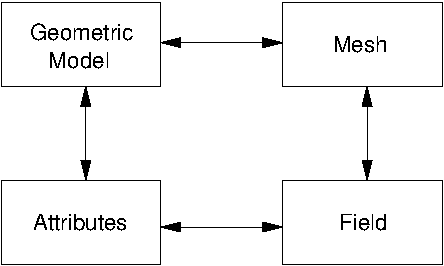
\includegraphics[width=2.5in]{../fig/compo_env}
\caption[The relationship between components of the geometry-based analysis environment]
{The relationship between components of the geometry-based analysis environment~\cite{beallthesis}}
\label{fig:compo}  % the \label command comes AFTER the caption
\end{figure}

%%%%%%%%%%%%%%%%%%%%%%%%%%%%%%%
\subsubsection{Geometric model}
%%%%%%%%%%%%%%%%%%%%%%%%%%%%%%%

\begin{figure}
\centering
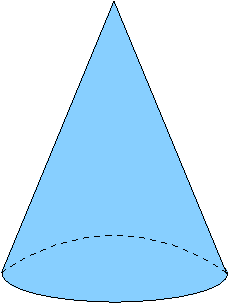
\includegraphics[height=1.3in]{../fig/manifold}\hspace{.5in}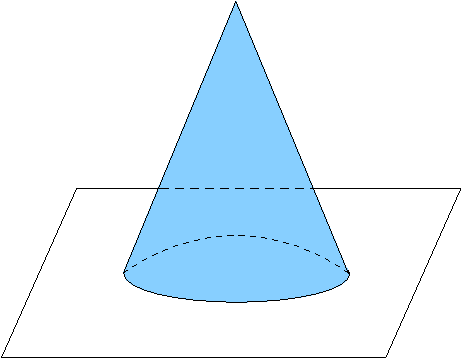
\includegraphics[height=1.5in]{../fig/nonmanifold}
\caption[Example of manifold and non-manifold models]
{Example of (left) manifold and (right) non-manifold models}
\label{fig:nonmanifold}  % the \label command comes AFTER the caption
\end{figure}

The most common geometric representation is a boundary representation. A general
representation of general non-manifold domains is the Radial Edge Data
Structure~\cite{weiler88}. Non-manifold models are common in engineering analyses. Simply speaking,
non-manifold models consist of general combinations of solids, surfaces, and
wires. Figure~\ref{fig:nonmanifold} illustrates examples of manifold and
non-manifold model.

In the boundary representation, the model is a hierarchy of topological entities
called regions, shells, faces, 
loops, edges, vertices, and in case of non-manifold models, use entities for vertices, edges, loops, and
faces.  %The use of a boundary representation is convenient for attribute
%association and mesh generation processes since the 
%boundaries of the model are explicitly represented.
The data structure implementing the geometric model supports operations
to find the various model entities that make up a model, information about which model
entities are adjacent to a given entity, operations relating to perform
geometric shape queries, and queries about what attributes are associated with model
entities.

%%%%%%%%%%%%%%%%%%%%%%%%%%%%%%%
\subsubsection{Attribute}
%%%%%%%%%%%%%%%%%%%%%%%%%%%%%%%

\begin{figure}
\centering
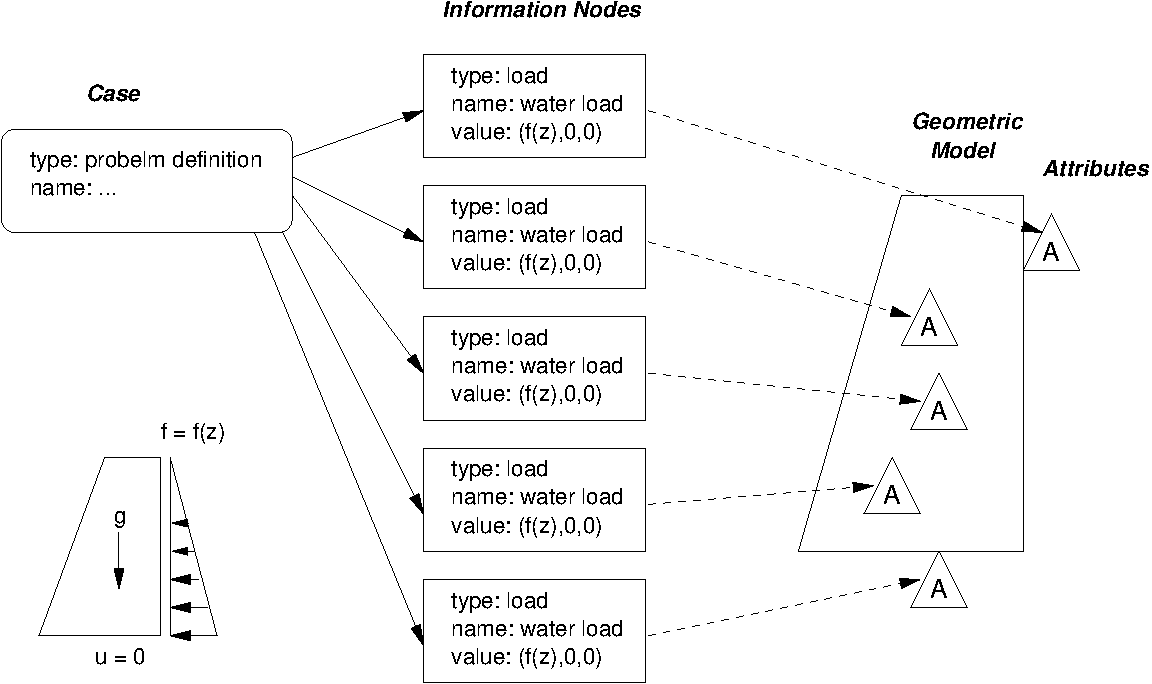
\includegraphics[width=4.5in]{../fig/attributes}
\caption[Example geometry-based problem definition]{Example geometry-based problem definition~\cite{beallthesis}}
\label{fig:dam}  % the \label command comes AFTER the caption
\end{figure}

In addition to geometric model, the definition of a problem requires other information that describes material
properties, loads and boundary conditions, etc. These
are described in terms of tensor-valued 
attributes and may vary in both space and time. Attributes are applied to geometric model entities. 

Figure~\ref{fig:dam} illustrates an example of a problem definition. The problem being modeled is a
dam subjected to loads due to gravity and due to the water behind the dam. There
is a set of attribute information nodes that are all under the attribute case
for the problem definition. When this case is associated with the geometric model,
attributes are created and attached to the individual model entities on which they act~\cite{beallthesis,
simmetrixweb}. The attributes are indicated by triangles with $A$'s inside of them.

%%%%%%%%%%%%%%%%%%%%%%%%%%%%%%%
\subsubsection{Mesh}
%%%%%%%%%%%%%%%%%%%%%%%%%%%%%%%

A mesh is a geometric discretization of a domain. With restrictions on the mesh
entity topology~\cite{beall97}, a mesh is represented with a hierarchy of
regions, faces, edges and vertices. Each mesh entity maintains a relation, called
geometric classification~\cite{beall97, shephard00}, to the model entity that it was
created to partially represent. Geometric classification allows an understanding of which 
attributes (e.g. boundary conditions or material properties) are related to the 
mesh entities and the how the solution relates back to the original problem
description, and is critical in mesh generation and adaptation~\cite{beallthesis, beall97, shephard00}. More discussion on the mesh representation is presented in $\S$2.2. 


In a geometry-based analysis environment, mesh data structures house the
discretization of the domain, a mesh, and provide the mesh-level services to applications. 

%%%%%%%%%%%%%%%%%%%%%%%%%%%%%%%
\subsubsection{Field}
%%%%%%%%%%%%%%%%%%%%%%%%%%%%%%%

\begin{figure}
\centering
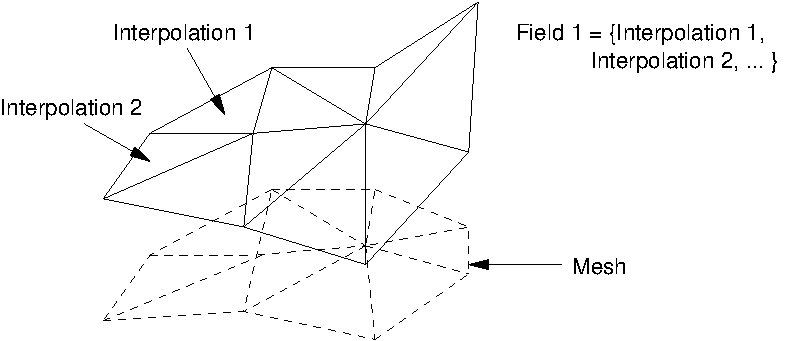
\includegraphics[width=3.5in]{../fig/field}
\caption[Representation of a field defined over a mesh]{Representation of a field defined over a mesh~\cite{beallthesis}}
\label{fig:field}  % the \label command comes AFTER the caption
\end{figure}

A field describes the variation of solution tensors over the mesh entities
discretizing one or more entities in a
geometric model. The spatial variation of the field is defined in terms of
mesh level distribution functions~\cite{beallthesis}.
Figure~\ref{fig:field} demonstrates the concept of a field written in terms of
$C^0$ interpolating distribution functions. 

%%%%%%%%%%%%%%%%%%%%%%%%%%%%%%%%%%%%%%%%%%%%%%%%%%%%%%%%%%%%%%
\subsection{General Topology-Based Mesh Data Structure}\label{ch:genmdb}
%%%%%%%%%%%%%%%%%%%%%%%%%%%%%%%%%%%%%%%%%%%%%%%%%%%%%%%%%%%%%%

The mesh consists of a collection of mesh entities of controlled size, shape,
and distribution. The relationships of the entities defining the mesh are well
described by topological adjacencies, which form a graph of the mesh~\cite{beall97, celes05, garimella02, aomd03}. A critical
capability needed by automated, adaptive geometry-based analysis 
procedures is to manipulate the mesh of the analysis domain. A mesh 
data structure is a toolbox that provides the mesh-level services to the
applications that create/use the mesh data. The differing needs of the
applications dictate that the database be able to answer to the needed
queries about the mesh. 
The five essential components of a general topology-based mesh data structure are:
topological entities, geometric classification, adjacencies between
entities~\cite{beall97}, entity set and arbitrary user data attachable to the topological entities or entity sets, referred as \emph{tag data}~\cite{itapsweb, Ollivier-etal06}.

%%%%%%%%%%%%%%%%%%%%%%%%%%%%%%%
\subsubsection{Topological entities}
%%%%%%%%%%%%%%%%%%%%%%%%%%%%%%%

Topology provides an unambiguous, shape-independent abstraction of the mesh.
With reasonable restrictions on the topology, a mesh is represented with only
the basic $0$ to \emph{d}
dimensional topological entities, where $d$ is the dimension of the domain of
the interest. The full set of mesh entities in 3D is \{\{M\{\Mz\}\}, \{M\{\Mo\}\}, \{M\{\Mt\}\},
\{M\{\Mth\}\}\}, where \{M\{\Md\}\}, $d=0,1,2,3$, are, respectively, the set of vertices,
edges, faces, and regions. Mesh edges, faces, and regions are bounded by the lower
order mesh entities. 

Restrictions on the topology of a mesh are:

\begin{itemize}
\item Regions and faces have no interior holes.
\item Each entity of order \emph{d} in a mesh, $M^d_i$, may use a particular
entity of lower order, \emph{p}, $M^p_j$, $p < d$, at most once.
\item For any entity $M^d_i$, there is the unique set of entities of order
$d-1$, $\{M^d_i\{M^{d-1}\}\}$ that are on the boundary of $M^d_i$. (Note, based
on mesh entity classification, it is possible to relax this restriction in the
case of equal order classification~\cite{beall97})
\end{itemize}

The first restriction means that regions may be represented by one shell of faces that
bounds them, and faces may be represented by one loop of edges that bounds them. The
second restriction allows the orientation of an entity to be defined in terms of
its boundary entities without introduction of use entities. The third
restriction means that an interior entity is uniquely specified by its bounding entities.


%%%%%%%%%%%%%%%%%%%%%%%%%%%%%%%
\subsubsection{Geometric classification}
%%%%%%%%%%%%%%%%%%%%%%%%%%%%%%%

The linkage of the mesh to the geometric model is critical for mesh generation and adaptation 
procedures since it allows the specification of analysis 
attributes in terms of the original geometric model, the proper approximation of
the geometry during mesh adaptation and supports direct links to
the geometric shape information of the original domain need to improve geometric
approximation and useful in p-version element integration~\cite{beallthesis, beall97, shephard00}. 

\begin{figure}
\centering
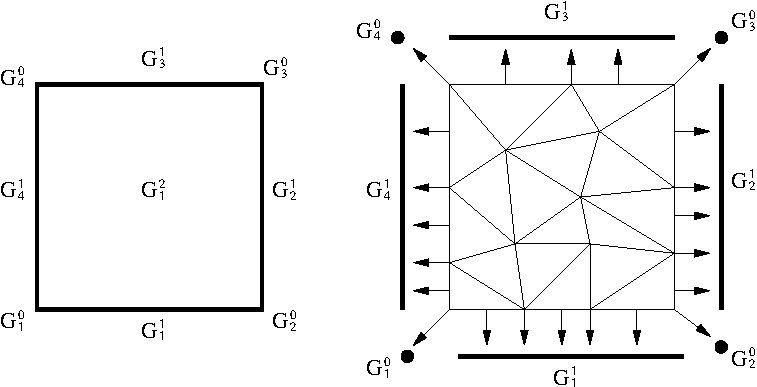
\includegraphics[width=4in]{../fig/gclas}
\caption[Example of simple model and mesh showing their association via geometric classification]
{Example of simple model(left) and mesh(right) showing
their association via geometric classification~\cite{simmetrixweb}} 
\label{gclas}  % the \label command comes AFTER the caption
\end{figure}

The unique association of a mesh entity of dimension \di, \Mdii, to the
 geometric model entity of dimension \djj, $G^{d_j}_j$, $d_i \le d_j$, on which
 it lies is termed geometric classification, and is denoted \Mdiib\clas\blk
 $G^{d_j}_j$, where the classification symbol, \clas,
indicates that the left hand entity, or a set of entities, is classified on the right hand entity. In Figure \ref{gclas}, a mesh of simple square model with entities labeled
is shown with arrows indicating the classification of the mesh entities onto the model
entities. All of the interior mesh faces, mesh edges, and mesh vertices are classified
on the model face $G^2_1$.

%%%%%%%%%%%%%%%%%%%%%%%%%%%%%%%
\subsubsection{Adjacencies}
%%%%%%%%%%%%%%%%%%%%%%%%%%%%%%%
\begin{figure}
\centering
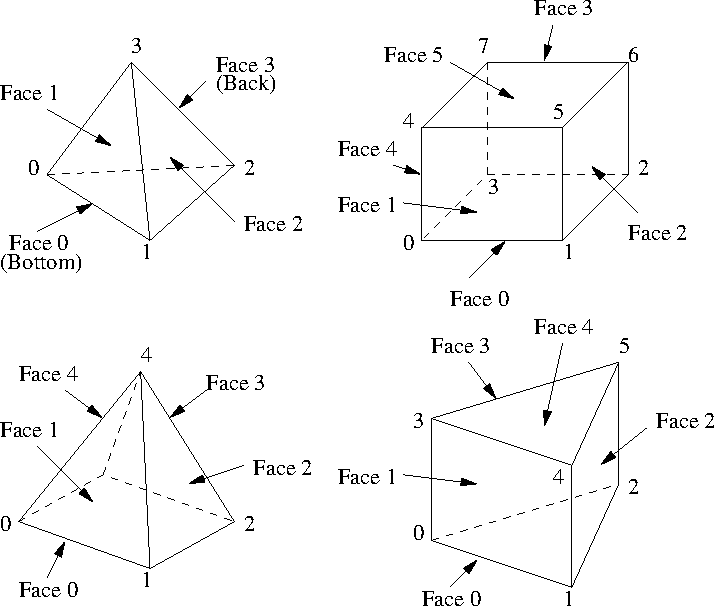
\includegraphics[width=4in]{../fig/rorder-vf}
\caption[Vertex and face order on a region]
{Vertex and face order on a region~\cite{simmetrixweb}}
\label{rorder1}  
\end{figure}

\begin{figure}
\centering
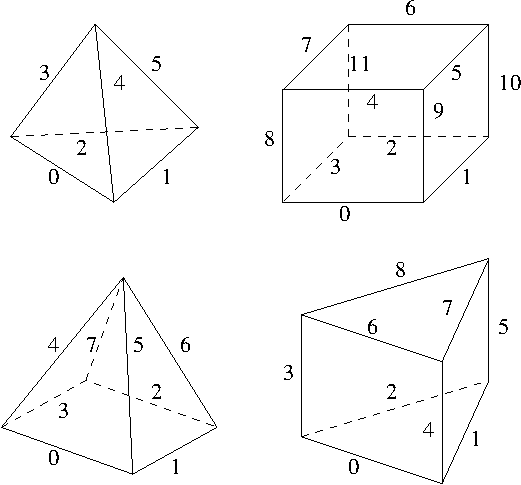
\includegraphics[width=3in]{../fig/rorder-e}
\caption[Edge order on a region]
{Edge order on a region~\cite{simmetrixweb}}
\label{rorder2}  
\end{figure}

\begin{figure}
\centering
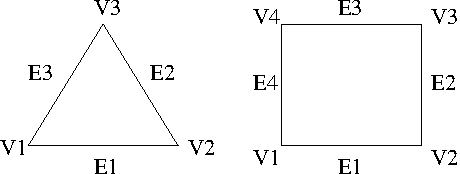
\includegraphics[width=3in]{../fig/forder}
\caption[Edge order on a face]
{Edge order on a face~\cite{simmetrixweb}}
\label{forder}
\end{figure}

\begin{figure}
\centering
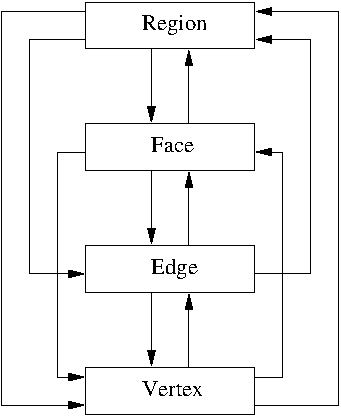
\includegraphics[width=1.5in]{../fig/12adj}
\caption[12 adjacencies possible in the mesh representation]
{12 adjacencies possible in the mesh representation~\cite{garimella02}}
\label{12adj}  % the \label command comes AFTER the caption
\end{figure}

Adjacencies describe how mesh entities connect to each other. For
an entity of dimension $d$, first-order adjacency returns all of
the mesh entities of dimension $q$, which are on the closure of the
entity for a downward adjacency ($d>q$), or for which the entity is
part of the closure for an upward adjacency ($d<q$). For denoting specific downward
first-order adjacent entity,
$M^d_i\{M^q\}_j$, the ordering conventions can be used to enforce the
order. Figure \ref{rorder1}, \ref{rorder2}, and \ref{forder} illustrate a
common canonical order of bounding entities. Figure~\ref{12adj} is an
adjacency graph that depicts 12 first-order adjacencies possible in 
the mesh data structure where a solid box and a solid arrow
denote, respectively, explicitly stored level of entities and explicitly stored adjacencies from
outgoing level to incoming level. In the adjacency graph, a solid box denotes that entities of the level are explicitly stored, and a solid arrow denotes that adjacencies from an outgoing level to an incoming level are maintained for the level of entities.

For an entity of dimension $d$, second-order adjacencies describe
all the mesh entities of dimension $q$ that share any adjacent
entities of dimension $b$, where $d \neq b$ and $b \neq q$. Second-order
adjacencies can be derived from first-order adjacencies. 

Examples of adjacency requests include: for a given face, the regions
on either side of the face (first-order upward); the vertices bounding
the face (first-order downward); and the faces that share any vertex
with a given face (second-order). 

%%%%%%%%%%%%%%%%%%%%%%%%%%%%%%%%%%%%%%%%%%%%%%%%%%%%%%%%%%%%%%
\subsubsection{Mesh Representation}\label{ch:meshrep}
%%%%%%%%%%%%%%%%%%%%%%%%%%%%%%%%%%%%%%%%%%%%%%%%%%%%%%%%%%%%%%
The mesh representation can be categorized with two criteria (i) full vs. reduced and (ii) complete vs. incomplete, resulting in 4 different groups~\cite{seolthesis}. 

If a mesh representation stores all $0$ to $d$ level entities explicitly, it is a $full$ representation, otherwise, it is a $reduced$ representation. \emph{Completeness of adjacency} indicates the ability of a mesh representation
to provide any type of adjacencies requested without involving an
operation dependent on the mesh size such as the global mesh search or mesh traversal.
Regardless of full or reduced, if all adjacency information is obtainable in
O(1) time (the first circle), the representation is \emph{complete}, otherwise it is \emph{incomplete}. 

The \emph{general} topology-based mesh data structures must satisfy completeness of adjacencies to support adaptive
analysis efficiently. It doesn't necessarily mean that all $d$ level entities and adjacencies need be explicitly stored in the representation so there are many representation options in the design of general topology-based mesh data structure. 
\begin{figure}
\centering
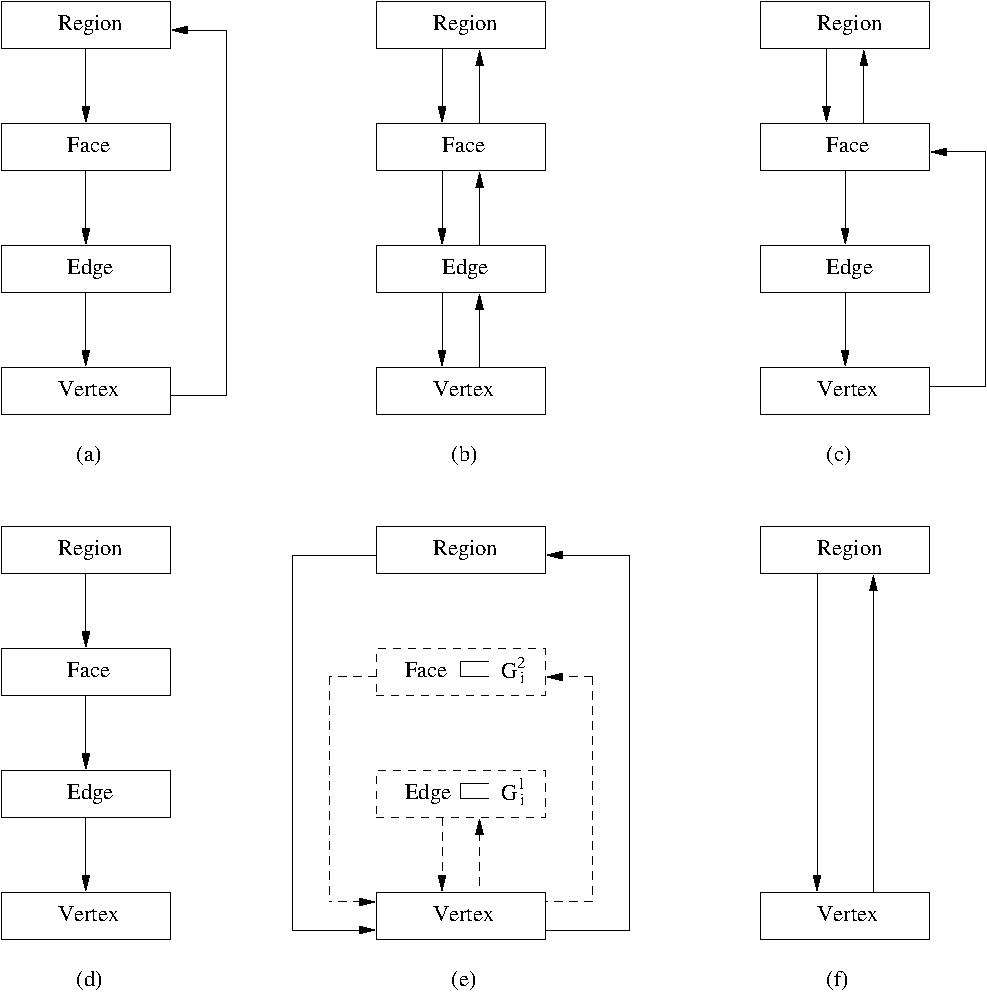
\includegraphics[width=4.2in]{./fig/6complete}
\caption{Example of 3D mesh representations}
\label{fig:6completeMR}  
\end{figure}

In the mesh representation graph, a dotted box denotes that among entities of the level, only equally
classified ones are explicitly stored, and a dotted arrow denotes that adjacencies
from an outgoing level to an incoming level are maintained only for the stored
entities.

In Figure \ref{fig:6completeMR} illustrates 6 mesh representations in 3D. Note that in the adjacency graph, a dotted box denotes that among entities of the level, only equally
classified ones are explicitly stored, and a dotted arrow denotes that adjacencies
from an outgoing level to an incoming level are maintained only for the stored
entities. (a) to (c) are full and complete due to all $0$ to $d$ levels of entities exist and the 12
adjacencies are obtainable in O(1) time either by direct access or local
traversal, (d) is full and incomplete
since it requires mesh level global search or traversal to get proper
adjacencies, (e) is reduced and complete, and (f) is reduced and incomplete. Representation (b) is \emph{the one-level adjacency representation} as it maintains adjacencies between entities one dimension apart. Representation (e) is \emph{the complete minimum sufficient representation} that
stores the minimum sufficient representation plus upward adjacencies from
vertices to their bounding entities of level $>$ 0. Representation
(f) is the classic mesh connectivity structure 
that describes the mesh only in terms of elements and nodes, and also has been used
for several finite element applications~\cite{beall97}.

For more discussions on mesh representations, see Reference ~\cite{seolthesis}.

%%%%%%%%%%%%%%%%%%%%%%%%%%%%%%%
\subsubsection{Entity set}
%%%%%%%%%%%%%%%%%%%%%%%%%%%%%%%

An entity set provides a mechanism for creating arbitrary groupings of entities for various purposes such as representing boundary layer, boundary condition and materials. Each entity set can be either of a set with unique entity or a list with insertion order preserved. The following are the functionalities of entity set to effectively support the application needs~\cite{itapsweb, Ollivier-etal06}.
 
\begin{itemize}
\item populating by addition or removal of entities from the set
\item traversal through an iterator with various conditions such as topology, and type of the entity
\item set boolean operations of subtraction, intersection, and union
\item relationships among entity sets: subset, parent/child
\end{itemize}

In parallel computing environment, the mesh is distributed over multiple parts across the processes. Therefore, there are two kinds of set available in distributed mesh.
\begin{itemize}
\item mesh set: entity set created in a mesh. entities in the set can be in different part.
  \begin{itemize}
    \item $L-SET$: a list type entity set created in mesh. Insertion order is preserved and an entity can be inserted multiple times.
    \item $S-SET$: a set type entity set created in mesh. Insertion order is not preserved and an entity can be inserted at most once.
\end{itemize}
\item  part set or $P-SET$: a set type entity set created in part. Insertion order is preserved and only entities ithout higher order adjacency can be inserted. 
\end{itemize}

Please be noted that entity set is not supported in the current PUMI release.

%%%%%%%%%%%%%%%%%%%%%%%%%%%%%%%
\subsubsection{Iterator}
%%%%%%%%%%%%%%%%%%%%%%%%%%%%%%%

Iterators are a generalization of pointers which are objects that point to other objects. Iterators are often used to iterate over a range of objects: if an iterator points to one element in a range, then it is possible to increment it so that it points to the next element~\cite{sgiweb}. 

Various kinds of iterators are desirable for efficient mesh entity traversal with various conditions such as entity dimension, entity topology, geometric classification. Furthermore, the iterator validity shall be guaranteed with mesh modification through entity creation/deletion.

%%%%%%%%%%%%%%%%%%%%%%%%%%%%%%%
\subsubsection{Tag}\label{tag}
%%%%%%%%%%%%%%%%%%%%%%%%%%%%%%%

A tag is a container of arbitrary data attachable to meshes, entities, and entity sets. Different values of a particular tag can be associated with mesh, entity, or entity set~\cite{itapsweb, Ollivier-etal06}. 

For efficient manipulation of tags and their association with meshes, entities and entity sets, tags consist of the following data.
\begin{itemize}
\item{tag name}: character string for identifying tag
\item{tag data}: data stored in the tag
\item{tag type}: data type for tag data \\
For better performance and management, five specialized tag types, integer, double, mesh entity, entity set and byte type data are supported through interface. If the tag data consists of multiple units (e.g. array of integer data), the size of tag data in byte and  the number of units are needed for efficient tag manipulation.
\item{tag size}: the number of units of \emph{tag type} in tag data
\item{tag byte}: the size of tag data in bytes
\end{itemize}

%%%%%%%%%%%%%%%%%%%%%%%%%%%%%%%
\subsection{S/W Structure}
%%%%%%%%%%%%%%%%%%%%%%%%%%%%%%%

\begin{figure}[!t]
\centering
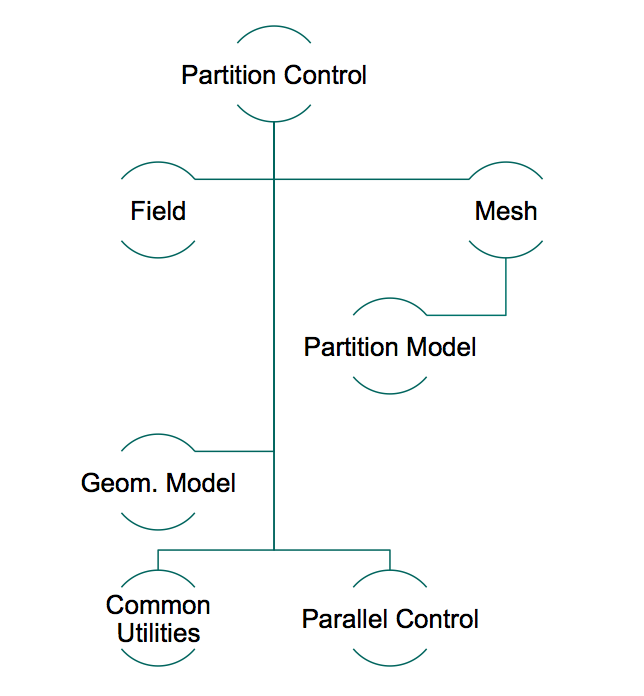
\includegraphics[width=3in]{fig/pumi.jpg} 
\caption{Software structure of PUMI}
\label{fig:pumi}
\end{figure}

In development, geometry-based analysis s/w is modularized based on the features and goals as component. Figure~\ref{fig:pumi} illustrates the software structure of PUMI consisting of the following seven components. % add some additional discussion of the interactions implied in the figure
\begin{itemize}
\item The \emph{common utility} component provides common utilities and services used in multiple other components such as iterator, set, and tag.
\item The \emph{parallel control} component provides parallel-specific utilities and services such as communications and architecture-aware operations.
\item The \emph{geometric model} component provides a uniform interface for querying geometric model representations. It uses common utility and parallel control component. 
\item The \emph{partition model} component is constructed based on the mesh distribution and provides mesh partitioning representation in topology to the mesh component for the support for efficient update/manipulation of mesh with respect to partitioning. 
\item The \emph{mesh} component provides the storage and management of distributed unstructured meshes. It uses all components except for  the field component.
\item The \emph{field} component provides the services for storage and management of solution information on the mesh. It uses common utility, parallel control and mesh components.
\item The \emph{partition control} component provides the services for improving mesh partitioning via graph partitioner or existing mesh information such as adajacencies.
\end{itemize}


PUMI consists of multiple libraries which are modularized based on supported features. 

\begin{itemize}
\item \texttt{pumi}: a library with API hearder file and PUMI error codes. PUMI error codes are defined in the file \texttt{pumi\_errorcode.h} and the API's are defined in the file \texttt{pumi.h}.
\item \texttt{pcu}: a library with parallel control and comminication. The header file is obtained in \texttt{PCU.h}.
\item \texttt{gmi}: a library with SCOREC-formatted geometric model implementation. 
\item \texttt{mds}: a library with SCOREC-formatted mesh implementation. 
\item \texttt{apf}: a library with field, common mesh interface, common geometric model interface, interations between geometric model and mesh implmentation, etc. The header file is obtained in \texttt{apf.h}.
\item \texttt{parma}: a library with adjacency-based mesh partitioning functions. The header file is obtained in \texttt{parma.h}.
\item \texttt{zoltan}: a library to support interaction with Zoltan~\cite{ZoltanIsorropiaOverview2012, ZoltanOverviewArticle2002} graph partitioning S/W.
\end{itemize}


\section{Parallel Control and Communication}  

The PCU (Parallel Control Utility) is a library for parallel computation based on
MPI with additional support for hybrid MPI/thread environments. PCU is included in PUMI to support needed parallel controls and communication for operations with distributed meshes and model.

The PCU provides three things to users:

\begin{enumerate}
\item A phased message passing API
\item A thread management API
\item Support for phased message passing between threads instead of processes
\end{enumerate}

Phased message passing is similar to Bulk Synchronous Parallel,
but is implemented more efficiently.
All messages are exchanged in a phase, which is a collective operation involving
all threads in the parallel program.
During a phase, the following events happen in sequence:

\begin{enumerate}
\item All threads send non-blocking messages to other threads
\item All threads receive all messages sent to them during this phase
\end{enumerate}

PCU provides termination detection, which is the ability to detect when all messages
have been received without prior knowledge of which threads are sending to which.

To write hybrid MPI/thread programs, PCU provides a function that creates threads
within an MPI process, similar to the way mpirun creates multiple processes.
PCU assigns ranks to these threads and has them each run the same function, with
thread-specific input arguments to the function.

Once a program has created threads using PCU, it can call the phased message passing
API from within threads, which will behave as if each thread were an MPI process.
Threads have unique ranks and can send messages to one another, regardless of which
process they are in.



%%%%%%%%%%%%%%%%%%%%%%%%%%%%%%%%%%%%%%%%%%%%%%%%%%%%%%%%%%%%%%%%%%
\section{Geometric Model}  

PUMI geometric model interface supports the ability to interrogate solid models for topological adjacency and geometric shape information.

The geometric model representation used by PUMI is a boundary representation based on the Radial Edge Data Structure~\cite{weiler88}. In this representation the model is a hierarchy of topological entities called regions, shells, faces, loops, edges and vertices. This representation is general and is capable of representing non-manifold models that are common in engineering analyses. The use of a boundary representation is convenient for the association of problem attributes (e.g., loads, material properties and boundary conditions) and mesh generation control information since the entities defining the model are explicitly represented. 

The classes used to represent the geometric model support operations to find the various model entities that make up a model and to find which model entities are adjacent to a given entity. Other operations relating to performing geometric queries are also supported.

%%%%%%%%%%%%%%%%%%%%%%%%%%%%%%%%%%%%%%%%%%%%%%%%%%%%%%%%%%%%%%%%%%



%%%%%%%%%%%%%%%%%%%%%%%%%%%%%%%%%%%%%%%%%%%%%%%%%%%%%%%%%%%%%%%%%%
\section{Distributed Mesh Management}  
%%%%%%%%%%%%%%%%%%%%%%%%%%%%%%%%%%%%%%%%%%%%%%%%%%%%%%%%%%%%%%%%%%

A distributed mesh data structure is an infrastructure executing 
underneath providing all parallel mesh-based operations needed to support
parallel adaptive analysis. An efficient and scalable distributed mesh data structure is
 mandatory to achieve performance since it strongly influences
the overall performance of adaptive mesh-based simulations. In addition to
the general mesh-based operations, the distributed
mesh data structure must support $(i)$ efficient communication between
 entities duplicated over multiple processes, $(ii)$ migration of entities
 between processes, and $(iii)$ dynamic load balancing. 

This chapter presents the concept and functionalties of distributed mesh management. $\S$\ref{pmodel} describes a partition model that is developed in FMDB for the purpose of effectively meeting the specific functionalities of distributed meshes~\cite{seolthesis, fmdb06}. The readers not interested in the internal design and implementation of the distributed meshes in FMDB might skip $\S$\ref{pmodel}

%%%%%%%%%%%%%%%%%%%%%%%%%%%%%%%%%%%%%%%%%%%%
% SECTION 4.1	
\subsection{Distributed Mesh Representation}  
%%%%%%%%%%%%%%%%%%%%%%%%%%%%%%%%%%%%%%%%%%%%

\begin{figure}
\centering
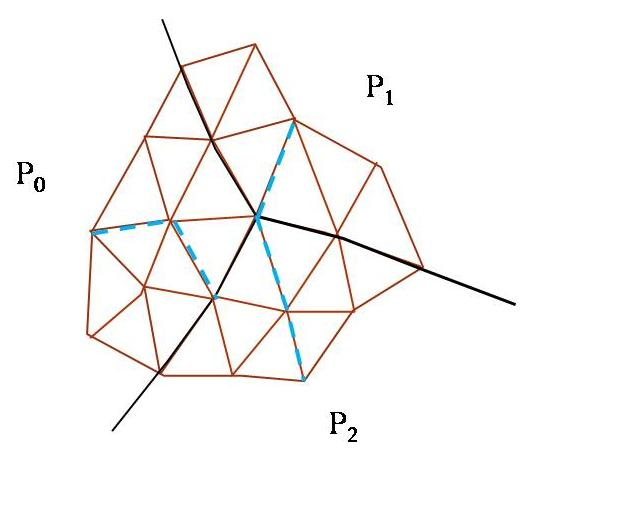
\includegraphics[width=3in]{../fig/distMesh1.jpg}
\caption[Distributed mesh on three processes with two parts per process]{Distributed mesh on three processes $P_0$, $P_1$ and $P_2$ with two parts per each process}
\label{distMesh1}  % the \label command comes AFTER the caption
\end{figure}

\emph{A distributed mesh} is a mesh divided into parts for distribution
over a set of processes for specific reasons, for example, parallel computation.

\begin{description}
\item[Definition 3.1] \emph{Part}\\
A part consists of the set of mesh entities assigned to a
process. For each part, a unique global part id within an entire system and a local part id within a process can be given.
\end{description}

Each part will be treated as a serial mesh with the addition of mesh
part boundaries to describe groups of mesh entities that are on inter-part boundaries. Mesh entities on part boundaries are
duplicated on all parts on which they are used in adjacency relations. Mesh entities not on the part boundary exist on only one part and referred as \emph{internal entities}. In implementation, for effective manipulation of multiple parts on each process, a single mesh data is defined on each process so multiple parts are contained in the mesh data where the mesh data is assigned to a process. The mesh data defined on each process is referred as \emph{mesh instance}. Figure~\ref{distMesh1} depicts a mesh that is distributed on 6 parts where the mesh instance on each process has two parts respectively. The dashed lines are \emph{part boundaries} within a process and the solid black lines are \emph{part boundaries} between the processes. The vertices and edges on part boundaries are duplicated on multiple parts.

In order to simply denote a set of parts where a mesh entity physically exist, termed \emph{residence part set}, we define an operator {\RP}. 

\begin{description}
\item[Definition 3.2] \emph{Residence part set operator \RP\Ls\Mdi\Rs} \\
An operator that returns a set of global part id(s) where \Mdib exists. 
\end{description}

%For any entity \Mdi\blk not on the boundary of any other mesh entities and on partition
%$p$, \RP\Ls\Mdi\Rs\blk returns \{$p$\} since when the entity is not on the boundary of any
%other mesh entities of higher order, its bounding part is determined
%simply to be the partition where it resides.  For entity \Mdi\blk on the
%boundary of higher order mesh entities, \RP\Ls\Mdi\Rs\blk is determined by the
%resident partition equation.

\begin{description}
\item[Definition 3.3] \emph{Residence part equation of \Mdi} \\
If \{$M^d_i$\{$M^q$\}\} $= \emptyset$, $d<q$, \RP$[$\Mdi\Rs\blk = \{$p$\} where $p$
is the id of a part where $M^d_i$ exists. Otherwise, \RP$[$\Mdi\Rs\blk = $\cup$ \RP$[$$M^q_j$ $\mid$ $M^d_i$ $\in$
\{$\partial$($M^q_j$)\}\Rs. %\\
%: For entity $M^q_k$, every \Mdib $\in$ \{$\partial$($M^q_k$)\} is on \RP\Ls$M^q_k$\Rs.
%Therefore, \Mdib exists wherever the mesh entity, $M^q_k$, it bounds exists.
\end{description}

For any entity \Mdi\blk not on the part boundary of any higher order mesh entities and on part
$p$, \RP$[$\Mdi\Rs\blk returns \{$p$\} since when the entity is not on the boundary of any
other mesh entities of higher order, its residence part set is determined simply to be the part where it resides.
If entity \Mdi\blk is on the boundary of other higher order mesh entities, \Mdi\blk is duplicated on multiple parts depending on the residence part set of its bounding entities since \Mdib exists wherever a mesh entity it bounds exists.

Therefore, the residence part set of \Mdi\blk is the union
of residence part set of all entities that it bounds. For a mesh topology
where the entities of order $d>0$ are 
bounded by entities of order $d-1$, \RP\Ls\Mdi\Rs\blk is determined to be
\{p\} if \{\Mdi\{\Mdpok\}\} $= \emptyset$. Otherwise, \RP\Ls\Mdi\Rs\blk is $\cup$ \RP\Ls$M^{d+1}_k$ $\mid$
$M^d_i$ $\in$ \{$\partial$($M^{d+1}_k$)\}\Rs. For instance, for the
3D non-manifold mesh depicted in Figure~\ref{pmesh3procs}, where $M^3_1$ and $M^2_1$
are on $P_0$, $M^3_2$ and $M^2_2$ are on $P_1$ and $M^1_1$ is on $P_2$, residence part set of $M^0_1$ are \{$P_0$, $P_1$, $P_2$\} since the union of residence part set of its bounding
edges, \{$M^1_1$, $M^1_2$, $M^1_3$, $M^1_4$, $M^1_5$, $M^1_6$\}, are \{$P_0$, $P_1$,
$P_2$\}. 

\begin{figure}
\centering
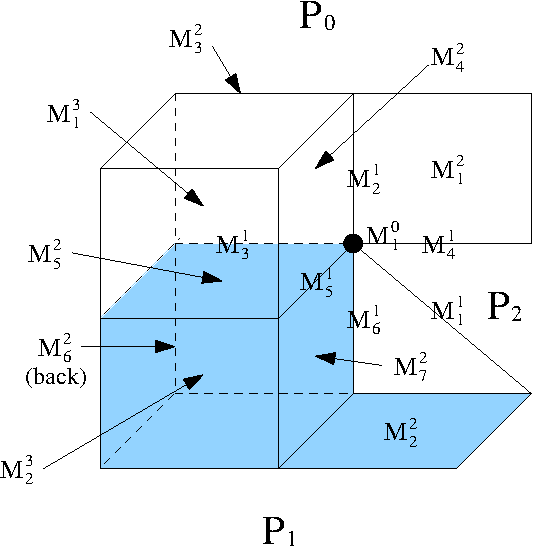
\includegraphics[width=2.5in]{../fig/PO}
\caption{Example 3D mesh distributed on three parts}
\label{pmesh3procs}  
\end{figure}

To migrate mesh entities to other parts, the destination part id's of
mesh entities must be specified before moving the mesh
entities. The residence part set equation implies that once the destination
part id of a \Mdi\blk that is not on its boundary of any other
mesh entities is set, the other entities needed to migrate are determined by
the entities it bounds. Thus, a mesh entity that is not on the boundary of any higher order mesh entities is the basic
unit to assign the destination part id in the mesh migration procedure.
 
\begin{description}
\item[Definition 3.4] \emph{Partition object}\\
The basic unit to which a destination part id is assigned. The full set of partition objects is
the set of mesh entities that are not part of the boundary of any higher order mesh
entities. In a 3D mesh, this includes all mesh regions, the mesh faces not bounded
by any mesh regions, the mesh edges not bounded by any mesh faces or regions, and mesh vertices not
bounded by any mesh edges, faces or regions. A set of unique mesh entities refered as entity set can also be a partition object if designated to be a migration unit.
\end{description}

In case of a manifold model, partition objects are all mesh
regions in 3D and all mesh faces in 2D. In case of a non-manifold model, the careful
lookup for entities not being bounded is required 
over the entities of one specific dimension. For example, partition objects of the mesh in Figure~\ref{pmesh3procs} are
$M^1_1$, $M^2_1$, $M^2_2$, $M^3_1$, and $M^3_2$. 

%%%%%%%%%%%%%%%%%%%%%%%%%%%%%%%%%%%%%%
\subsection{Functional Requirements}\label{ch:distmesh:req} 
%%%%%%%%%%%%%%%%%%%%%%%%%%%%%%%%%%%%%%

\subsubsection{Communication links}

Mesh entities on the part boundaries (shortly, part boundary entities) must be aware of where they are duplicated. 

\begin{description}
\item[Definition 3.5] \emph{Remote part}\\
Non-self part\footnote{A part that is not in the current local
part} where a mesh entity is duplicated.
\item[Definition 3.6] \emph{Remote copy}\\
Non-owned part boundary entities, in other words, the memory location of a mesh entity duplicated on remote part. 
\end{description}

\subsubsection{Ownership}

In parallel adaptive analysis, the mesh and its partitioning can change thousands of time
during the simulation~\cite{adapt06, deCougny-Shephard99, Oliker-etal00, Shep-etal97}. Therefore, at the mesh functionality 
level, an efficient mechanism to update the mesh partitioning and keep the links
between parts updated are mandatory to achieve scalability.

For entities on part boundaries duplicated on multiple parts, it is beneficial to
assign a specific part as the owner with charge of modification, communication or computation of the copies. For the purpose of simple denotation, a part bounday entity owned by the self part is referred as \emph{owner} of other entities copied on other parts.

\begin{figure}
\centering
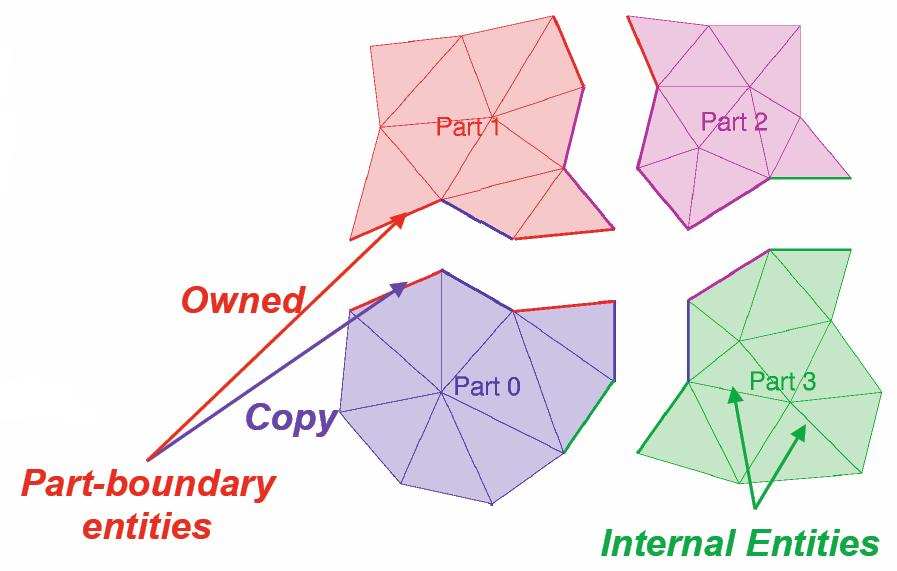
\includegraphics[width=3.5in]{../fig/distMesh2.jpg}
\caption[A distributed mesh on four processes with one part per process]{A distributed mesh on four processes with one part per process~\cite{itapsweb}}
\label{distMesh2}  % the \label command comes AFTER the caption
\end{figure}

Figure~\ref{distMesh2} depicts a mesh that is distributed on four processes with a single part per process. Entities on part boundaries are either of owner or copies. Internal entities are owners.

\subsubsection{Ghosting}

To avoid communications between the parts, it is beneficial to support the ability to have a copy of non-part boundary entities on other part, referred as $ghosting$~\cite{itapsweb}.

\begin{description}
\item[Definition 3.7] \emph{Ghost copy or ghost entity}\\
Non-owned, non-part-boundary entity in a part
\end{description}

\begin{figure}
\centering
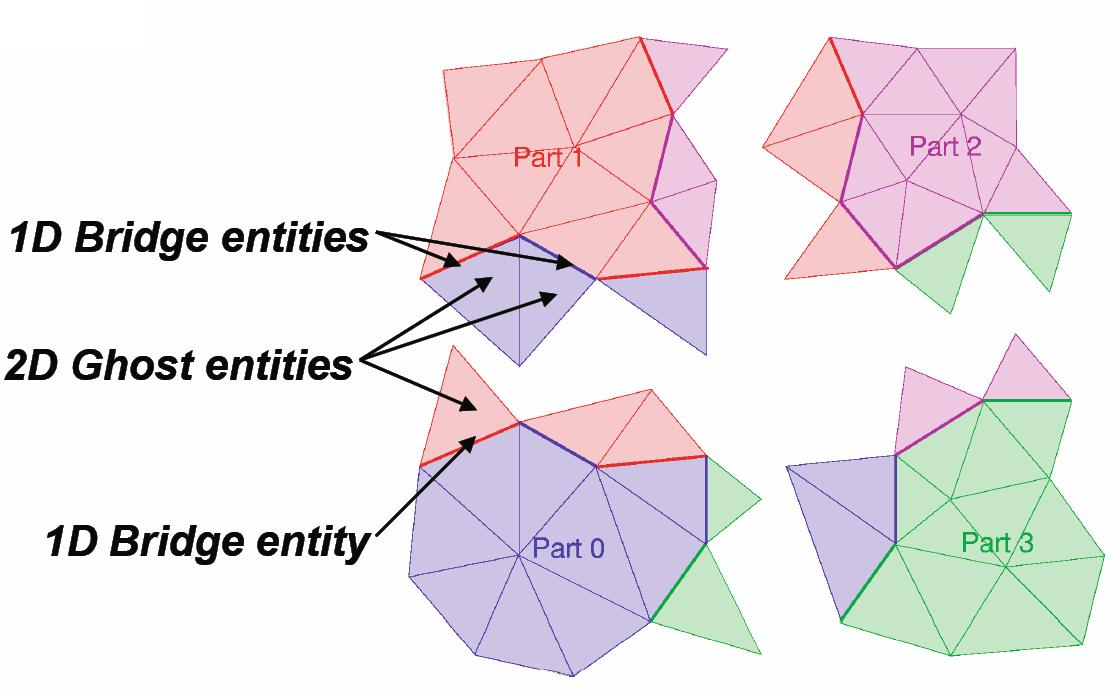
\includegraphics[width=3.7in]{../fig/ghost2.jpg}
\caption[A distributed mesh on four parts with ghost entities]{A distributed mesh on four parts with ghost entities~\cite{itapsweb}}
\label{ghost}  % the \label command comes AFTER the caption
\end{figure}

Figure~\ref{ghost} depicts a distributed mesh on four parts with ghost entities along the part boundaries. Similar to ownership of part boundary entities, the original owner entity is designated as \emph{owner} of all ghost copies.

To perform a layer-based ghosting, four input parameters are needed:
\begin{itemize}
\item bridge (entity) dimension
\item ghost (entity) dimension
\item the number of layers
\item a true/false flag indicating whether to include non-owned part boundary entities will be included for bridge entities. If true, all part boundary entities of bridge dimension are considered to construct ghost layer(s). If false, only $owned$ part boundary entities of bridge dimension are considered.
\end{itemize}

Ghost entities are specified through a \emph{bridge} dimension.  The number of layers is measured from the inter-part interfaces.  For example, to get two layers of region entities in the ghost layer, measured from faces on the interface, bridge dimension, ghost dimention, and the number of layers shall be, respectively, 2, 3, 2. The number of layers specified is with respect to the global mesh, that is, ghosting may extend beyond a single neighboring process if the number of layers is high.

In Figure~\ref{ghost}, The input parameters of ghosting (bridge dimension, ghost dimension, the number of layers and a flag) are $[1, 2, 1, true]$.

\begin{figure}
\centering
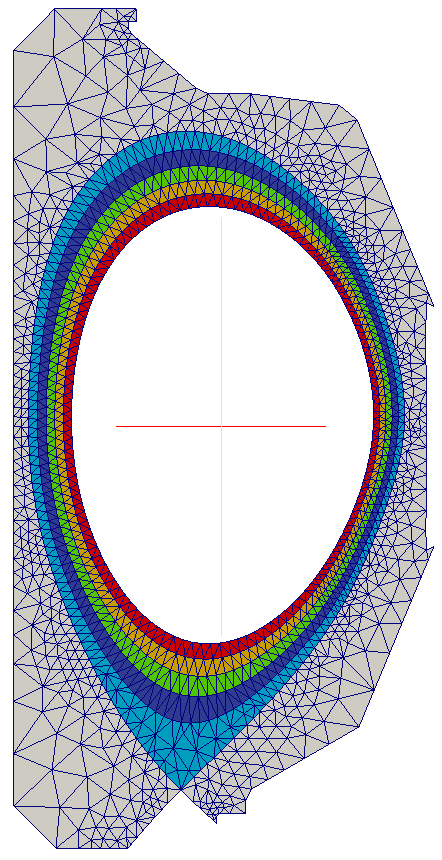
\includegraphics[width=1.5in]{./fig/part17-22.png}\hspace{1cm}
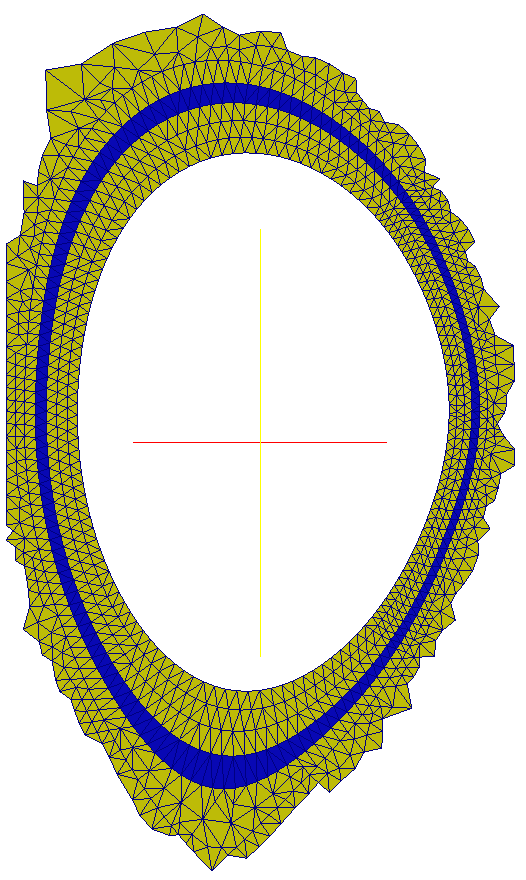
\includegraphics[width=1.7in]{./fig/part20-ghosted-copy}\hspace{1cm}
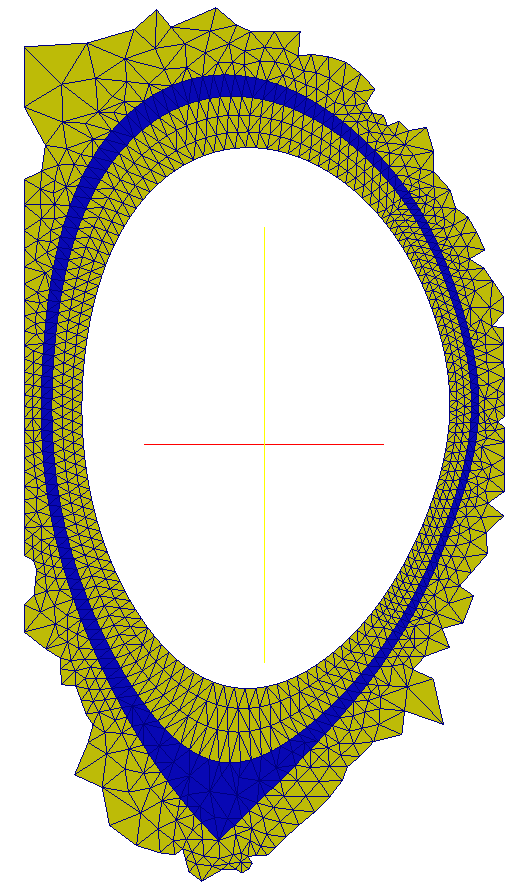
\includegraphics[width=1.7in]{./fig/part21-ghosted-copy}\hspace{1cm}
\caption{3-layer ghosting: (left to right) initial 6-part mesh, part 3 with 3 ghost layers, and part 4 with 3 ghost layers}
\label{xgc}  % the \label command comes AFTER the caption
\end{figure}

The left figure in Figure~\ref{xgc} depicts 6-part distributed mesh. The parts 0 to 5 are colored in red, orange, green, blue, turquoise, and gray respectively. The middle and right figure in Figure~\ref{xgc} illustrate the part 3 and part 4 with 3 ghost layers, where the original mesh entities are colored in blue and the ghost copies are colored in yellow. The input parameters of ghosting procedure are $[0, 2, 3, true]$.

%%%%%%%%%%%%%%%%%%%%%%%%%%%%%%%%%%%%%%%%%%%%
\subsubsection{Migration} 
%%%%%%%%%%%%%%%%%%%%%%%%%%%%%%%%%%%%%%%%%%%%

For effective management of distributed mesh with multiple parts per process, the following migration procedures are needed.

\begin{itemize}
\item Migrating entities and entity sets between parts with tag
\item Migrating whole parts between processes
\item Redistributing mesh. For example, splitting $n$ part mesh to $m$ parts, $n$ $\neq$ $m$, to load the mesh on an $m$ process machine.
\end{itemize}

%%%%%%%%%%%%%%%%%%%%%%%%%%%%%%%%%%%%%%%%%%%%
% SECTION 4.2
\subsection{A Partition Model}\label{pmodel}
%%%%%%%%%%%%%%%%%%%%%%%%%%%%%%%%%%%%%%%%%%%%

\begin{figure}
\centering
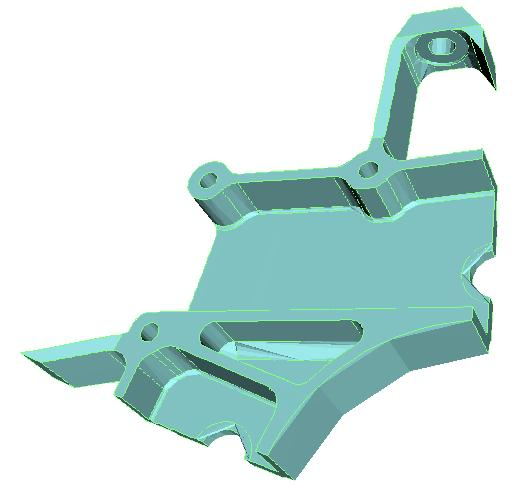
\includegraphics[width=1.9in]{../fig/hub_model.jpg}
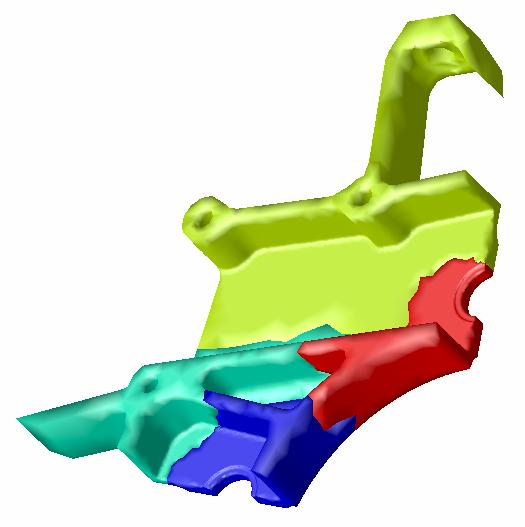
\includegraphics[width=1.9in]{../fig/hub_np4_pmodel.jpg}
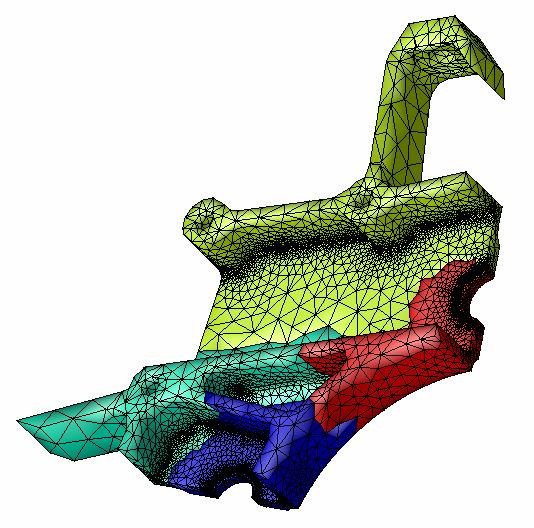
\includegraphics[width=1.9in]{../fig/hub_np4.jpg}
\caption[Hierarchy of domain decomposition]{Hierarchy of domain decomposition: (left to right) geometry model, partition model, and distributed mesh on 4 processes}
\label{torus}
\end{figure}

To meet the goals and functionalities of distributed meshes, a partition model has been
developed between the mesh and the geometric model. As illustrated in
Figure~\ref{torus}, the partition model can be
viewed as a part of hierarchical domain 
decomposition. Its purpose is to represent mesh
partitioning in topology and support mesh-level parallel 
operations through inter-part boundary links with ease. 

The specific implementation is the parallel extension of the unstructured mesh representation, such that standard mesh entities and adjacencies are used on processes only with the addition of the partition entity information needed to support all operations across multiple processes.

The partition model introduces a set of topological entities that represents the collections of mesh entities based on their location with
respect to the partitioning. Grouping mesh entities to define a partition entity
can be done with multiple criteria based on the level of functionalities and needs of distributed meshes. These constructs are consistent with the ITAPS iMeshP specification~\cite{itapsweb}.

At a minimum, \emph{residence part set} must be a criterion to be
able to support the inter-part communications. \emph{Connectivity} between entities is also desirable for a criterion to
support operations quickly and can be used optionally. Two mesh entities are $connected$ if they are on the same part and reachable via adjacency operations. The  connectivity is expensive but useful in representing separate  chunks in a part. It enables diagnoses of the quality of mesh partitioning immediately at the partition model level. In our implementation, for the efficiency purpose, only residence part set is used for the criterion. 

\begin{description}
\item[Definition 2.8] \emph{Partition (model) entity}\\
A topological entity in the partition model, \Pdi, which
represents a group of mesh entities of dimension $d$, that have the
same \RP. Each partition model entity is uniquely determined by \RP. 
\end{description}

Each partition model entity stores dimension, id, residence part set, and
the owning part. From a mesh entity level, by keeping proper relation to the
partition model entity, all needed services to represent mesh partitioning and support
inter-part communications are easily supported. 

\begin{description}
\item[Definition 2.9] \emph{Partition classification}\\
The unique association of mesh topological entities of dimension \di, \Mdii, to the topological entity of the
partition model of dimension \djj, \Pdjjb where $d_i \le d_j$, on which it lies is termed partition
classification and is denoted \Mdiib\clasb $P^{d_j}_j$.

\item[Definition 2.10] \emph{Reverse partition classification}\\
For each partition entity, the set of equal order mesh entities classified on that
entity defines the reverse partition classification for the partition model
entity. The reverse partition classification
is denoted as RC(\Pdj) = \{\Mdib $\mid$ \Mdib\clasb\Pdj\}. 
\end{description}

Figure~\ref{fig:pmeshwithpclas} illustrates a 3D distributed mesh with mesh entities labeled
with arrows indicating the partition classification of the entities onto the
partition model entities and its associated partition model. The mesh
vertices and edges on the thick black lines are classified on
partition edge $P^1_1$. The mesh
vertices, edges and faces on the shaded
planes are classified on the partition faces pointed with each arrow. The remaining
mesh entities are non-part boundary 
entities, therefore they are classified on the partition regions. Note the reverse
classification returns only the same order mesh entities. The reverse partition classification of
$P^1_1$ returns mesh edges located 
on the thick black lines, and the reverse partition classification of partition
face $P^2_i$ returns mesh faces on the shaded planes.

\begin{figure}
\centering
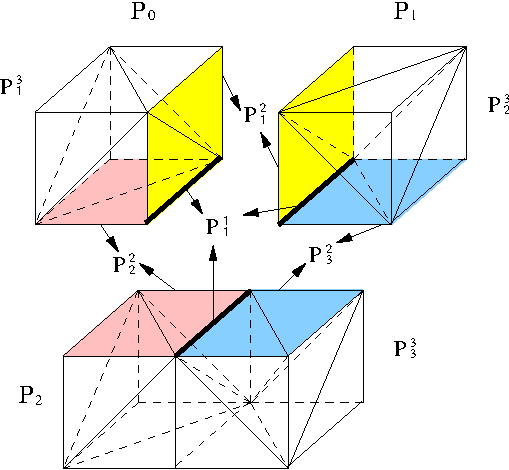
\includegraphics[height=2.5in]{../fig/pmesh3Dpclas2}\hspace{.3in}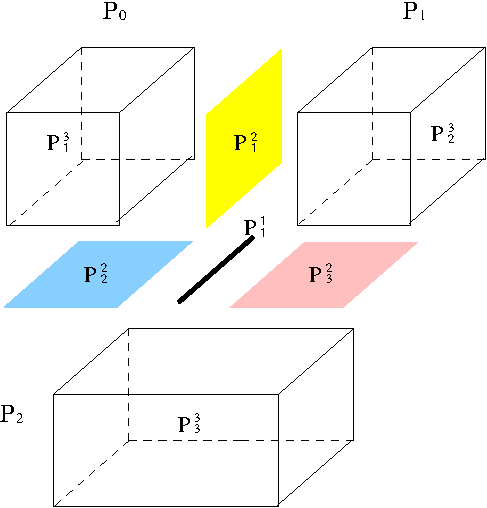
\includegraphics[height=2.5in]{../fig/pmodel3D}\\
\vspace{5pt}(a) distributed mesh \hspace{1in}(b) partition model\\
\vspace{7pt}
\caption{Distributed mesh and its association with the partition model via partition classifications}
\label{fig:pmeshwithpclas}
\end{figure}


%%%%%%%%%%%%%%%%%%%%%%%%%%%%%%%%%%%%%%%%%%%%%%%%%%%%%%%%%%%%%%%%%%%
\section{Mesh Partition Control}  
%%%%%%%%%%%%%%%%%%%%%%%%%%%%%%%%%%%%%%%%%%%%%%%%%%%%%%%%%%%%%%%%%%

This section discusses the issues with mesh partitioning and presents the background concept and goal of mesh partition control component.

Please be noted that the two libraries \emph{parma} and \emph{pumi$\_$field} are under development so not available in the current PUMI distribution. Please check pumi web page \textit{http://www.scorec.rpi.edu/pumi} for the release update.



\section{Interface Structure}

The PUMI API's are provided in the file \texttt{``pumi.h''}. Please be noted that in the current PUMI release, an entity set and multiple parts per process are not supported. Herein, with a single part per process, a mesh instance and a part handle are interchangeable.

\subsection{API naming convention}

PUMI API function name consists of two or three words connected with `$\_$'.

\begin{itemize}
\item the first word is ``pumi"
\item the second word is an operation target. If the operation target is system-wide, the operation target is ommited. For instance, the function that initializes the PUMI service is \emph{pumi}$\_$\emph{start}.
\item the third word is the operation description starting with a verb. For example, the function \emph{pumi}$\_$\emph{mesh}$\_$\emph{getNumEnt} returns the number of mesh entities with specific type. The function \emph{pumi}$\_$\emph{gent}$\_$\emph{getID} returns the global ID of geometric model entity.
\end{itemize}

The following are operation targets used in the second word.

\begin{itemize}
\item \textit{geom}: the api is performed on a geometric model
\item \textit{gent}: the api is performed on a geometric model entity
\item \textit{mesh}: the api is performed on a local mesh or global mesh
\item \textit{ghost}: the api performs ghosting functions
\item \textit{ment}: the api is performed on a mesh entity
\item \textit{tag}: the api is performed on a tag handle
\item \textit{field}: the api is performed on a field object
\item \textit{shape}: the api is performed on a field shape object
\item \textit{node}: the api is performed on a field node
\item \textit{numbering}: the api is performed on a numbering object
\end{itemize}

\subsection{Abbreviation}

Abbreviations may be used in API naming. See \textit{http://scorec.rpi.edu/wiki/Abbriviations} for more information.
 
\subsection{Data Types and Classes}

For a geometry, partition and mesh model, the term \emph{instance} is used to indicate the model data existing on each process. For example, a mesh instance on process \emph{i} means a pointer to a mesh data structure on process \emph{i}, in which all mesh entities on process \emph{i} are contained and from which they are accessible. For all other data such as entity and entity set, the term \emph{handle} is used to indicate the pointer to the data. For example, a mesh entity handle means a pointer to the mesh entity data. The predefined data type has a prefix \emph{p} to indicate the pointer data type.

The following are predefined data types used in the interface function parameters.

\begin{tabular}{lp{14cm}}	
	pGeom &		geometric model instance \\
	pGeomEnt &	geometric entity handle \\
	&\\
	pMesh &		mesh instance\\
        pMeshEnt &	mesh entity handle (i.e., vertex, edge, face, region) \\
        &\\
        pOwnership &    an ownership handle to allow user-defined ownership rule for part boundary entities\\
        Vector3 & 	an array of three doubles to hold the coordinate information of node\\
        Adjacent & 	an array of entities to hold the adjacency\\
        EntityVector  &    std::vector of mesh entity handle (pMeshEnt) \\
        Copies &          std::map of part ID (int) and mesh entity handle (pMeshEnt) to hold remote or ghost copies \\
        Parts  &          std::set of part ID (int) \\
	&\\
        pTag &          tag handle for geometric model\\
        pMeshTag &      tag handle for mesh\\
        &\\
	pGeomIter &		iterator traversing over global geometric model entities \\
        pMeshIter &          iterator traversing over local mesh entities\\
        pCopyIter &       iterator traversing \texttt{Copies} \\
        &\\
	pShape &	     shape function handle to define how the field nodes are distributed \\
        pField &             field handle\\
        pNumbering & numbering handle to assign local numbering to multiple degree of freedoms in field nodes \\
        pGlobalNumbering &   global numbering handle to assign global numbering to multiple degree of freedoms in field nodes\\
\end{tabular}	

The following classes are defined to support mesh re-distribution and ghosting.

\begin{tabular}{lp{14cm}}	
	Migration &	a class to define migration plan \\
	Distribution &	a class to define distribution plan \\
	Ghosting &	a class to define ghosting plan \\
\end{tabular}	

\subsection{Enumeration Types}

The enumeration type for tag data type is:

\begin{verbatim}
    enum PUMI_TagType {
        PUMI_DBL       = 0 /* double */,
        PUMI_INT,      /* 1 - integer */
        PUMI_LONG,     /* 2 - long integer */
        PUMI_ENT,      /* 3 - entity handle. Only for geometric model*/
        PUMI_SET,      /* 4 - set handle. NOT SUPPORTED */
        PUMI_PTR,      /* 5 - opaque pointer. Only for geometric model*/
        PUMI_STR,      /* 6 - string. NOT SUPPORTED */
        PUMI_BYTE      /* 7 - 1 byte character. Only for geometric model */
    }
\end{verbatim}\vspace{-1cm}\hspace{1cm}

For geometric model, the supported tag types are \emph{PUMI$\_$DBL}, \emph{PUMI$\_$INT}, \emph{PUMI$\_$LONG}, \emph{PUMI$\_$ENT}, \emph{PUMI$\_$PTR}, and \emph{PUMI$\_$BYTE}. For mesh, the supported tag types are \emph{PUMI$\_$DBL}, \emph{PUMI$\_$INT}, and \emph{PUMI$\_$LONG}.

The enumeration type for entity topology is:

\begin{verbatim}
enum PUMI_EntTopology {
  PUMI_VERTEX, 		// 0 
  PUMI_EDGE,   		// 1 
  PUMI_TRIANGLE, 	// 2 
  PUMI_QUAD,		// 3
  PUMI_TET,  		// 4
  PUMI_HEX,  		// 5 
  PUMI_PRISM, 		// 6
  PUMI_PYRAMID 		// 7
};
\end{verbatim}\vspace{-1cm}\hspace{1cm}

The enumeration type for field data type is:
\begin{verbatim}
enum PUMI_FieldType {
  PUMI_SCALAR, 		//  a single scalar value
  PUMI_VECTOR, 		// a 3D vector
  PUMI_MATRIX, 		// a 3x3 matrix 
  PUMI_PACKED 		// a user-defined set of components
};
\end{verbatim}\vspace{-1cm}\hspace{1cm}

\subsection{Error Codes}
If the API function returns an error code and the function succeeds, it returns 0,  otherwise, it returns a positive integer representing a type of error. The error codes are defined in \emph{pumi}$\_$\emph{errorcode.h}. 

\begin{verbatim}
 enum PUMI_ErrCode {
  PUMI_SUCCESS = 0, // no error
  PUMI_MESH_ALREADY_LOADED,
  PUMI_FILE_NOT_FOUND,
  PUMI_FILE_WRITE_ERROR,
  PUMI_NULL_ARRAY,
  PUMI_BAD_ARRAY_SIZE,
  PUMI_BAD_ARRAY_DIMENSION,
  PUMI_INVALID_ENTITY_HANDLE,
  PUMI_INVALID_ENTITY_COUNT,
  PUMI_INVALID_ENTITY_TYPE,
  PUMI_INVALID_ENTITY_TOPO,
  PUMI_BAD_TYPE_AND_TOPO,
  PUMI_ENTITY_CREATION_ERROR,
  PUMI_INVALID_TAG_HANDLE,
  PUMI_TAG_NOT_FOUND,
  PUMI_TAG_ALREADY_EXISTS,
  PUMI_TAG_IN_USE, // try to delete a tag that is in use
  PUMI_INVALID_SET_HANDLE,
  PUMI_INVALID_ITERATOR,
  PUMI_INVALID_ARGUMENT,
  PUMI_MEMORY_ALLOCATION_FAILED,
  PUMI_INVALID_MESH_INSTANCE,
  PUMI_INVALID_GEOM_MODEL,
  PUMI_INVALID_GEOM_CLAS,
  PUMI_INVALID_PTN_CLAS,
  PUMI_INVALID_REMOTE,
  PUMI_INVALID_MATCH,
  PUMI_INVALID_PART_HANDLE, 
  PUMI_INVALID_PART_ID,
  PUMI_INVALID_SET_TYPE,
  PUMI_INVALID_TAG_TYPE,
  PUMI_ENTITY_NOT_FOUND,
  PUMI_ENTITY_ALREADY_EXISTS,
  PUMI_REMOTE_NOT_FOUND,
  PUMI_GHOST_NOT_FOUND,
  PUMI_CB_ERROR,
  PUMI_NOT_SUPPORTED,
  PUMI_FAILURE, 
}
\end{verbatim}

\section{Comminication API's}

\emph{``PCU.h"} provides the API functions for parallel communications including MPI. 


%%%%%%%%%%%%%%%%%%%%%%%%%%%%%%%
\section{System-wide API's}
%%%%%%%%%%%%%%%%%%%%%%%%%%%%%%%

This section describes API functions and enumeration types which are not bounded with a specific geometric model or mesh data.

\begin{verbatim}
void pumi_start()		
\end{verbatim}
\vspace{-.5cm}\hspace{1cm}
	Initialize parallel services pertinent to PUMI.

\begin{verbatim}	
void pumi_finalize(bool /* in */ do_mpi_finalize=false)		
\end{verbatim}\vspace{-.5cm}\hspace{1cm}
	Finalize parallel services and clean the memory. If the input parameter \emph{do}$\_$\emph{mpi}$\_$\emph{finalize} is true, MPI finalization is performed as well. \emph{do}$\_$\emph{mpi}$\_$\emph{finalize} is optional (default: \emph{false}).

\begin{verbatim}
int pumi_size()
\end{verbatim}\vspace{-.5cm}\hspace{1cm}
	Return the number of processes.

\begin{verbatim}
int pumi_rank()
\end{verbatim}	
\vspace{-.5cm}\hspace{1cm}
	Return the MPI rank in communicator. Rank starts from 0. 

\begin{verbatim}
void pumi_sync()
\end{verbatim}\vspace{-.5cm}\hspace{1cm}
	Synchronize all processes in communicator

\begin{verbatim}
void pumi_printSys()
\end{verbatim}\vspace{-.5cm}\hspace{1cm}
	Print system information such as host name, processor, operating system, etc.\\
\emph{(Example)} Linux node10.borg.scorec.rpi.edu 2.6.9-89.ELsmp SMP Mon Jun 22 12:31:33 EDT 2009 x86$\_$64.

\begin{verbatim}
double pumi_getMem()
\end{verbatim}\vspace{-.5cm}\hspace{1cm}
	Return the heap memory increase (MB) on local process since \emph{pumi}$\_$\emph{start()}.

\begin{verbatim}
double pumi_getTime()
\end{verbatim}\vspace{-.5cm}\hspace{1cm}
	Return the current time in second.


\begin{verbatim}
void pumi_printTimeMem(
        const char* /* in */ msg, 
        double /* in */ time, 
        double /* in */ memory)
\end{verbatim}\vspace{-.5cm}\hspace{1cm}
        Display $``$\emph{msg}: \emph{time} (sec) and \emph{memory} (MB)$"$.


%%%%%%%%%%%%%%%%%%%%%%%%%%%%%%%
\section{Geometric Model API's}
%%%%%%%%%%%%%%%%%%%%%%%%%%%%%%%

This chapter describes geometric model related API functions.

%%%%%%%%%%%%%%%%%%%%%%%%%%%%%%%
\subsection{Model  managemant and interrogation}
%%%%%%%%%%%%%%%%%%%%%%%%%%%%%%%

\begin{verbatim}
pGeom pumi_geom_load(
        const char* /* in */ model_file_name, 
        const char* /* in */ model_type="mesh",
        void (*geom_load_fp)(const char*))
\end{verbatim}
\vspace{-.5cm}\hspace{1cm}
	Given geometric model file name and geometric model type (\textit{``mesh", ``null", ``analytic"}), create a model, load the model data from the file, and return a geometric model instance. If \emph{model}$\_$\emph{type} is not provided, the default is \emph{``mesh"}.

In case where a geometric model is \emph{NOT} available, \texttt{pumi$\_$geom$\_$load(NULL, ``null")} will generate a ``null" geometric model which mimicks the minimal geometric model behavior enough to support the PUMI.

In case of the analytic model, the user can provide a function pointer in the third argument, which creates analytic model entities. If the third argument is not provided for the analytic model, a set of analytic model entities can be created later via functions \emph{gmi}\_\emph{add}\_\emph{analytic}, \emph{gmi}\_\emph{add}\_\emph{analytic}\_\emph{region}, \emph{gmi}\_\emph{add}\_\emph{analytic}\_\emph{cell}, and \emph{gmi}\_\emph{add}\_\emph{analytic}\_\emph{reparam}. For the details of analytic model entity creation, see \emph{top}\_\emph{source}\_\emph{dir/gmi/gmi}\_\emph{analytic.h}.

\begin{verbatim}	
void pumi_geom_delete (pGeom /* in */ g)
\end{verbatim}\vspace{-.5cm}\hspace{1cm}	
Given a geometric model instance, delete the model instance and deallocate the memory.

\begin{verbatim}
void pumi_geom_freeze(pGeom /* in */ g) 
\end{verbatim}
\vspace{-.5cm}\hspace{1cm}
In some special cases, the model entities can be created by users or derived from the mesh. 
In such cases, when the model construction is completed, the function \emph{pumi}\_\emph{geom}\_\emph{freeze} has to be called to update the internal data of the geometric model accordingly. This function finalizes the geometric model so no more model entity can be created afterwards.

\begin{verbatim}
int pumi_geom_getNumEnt(
        pGeom /* in */ g, 
        int /* in */ d)
\end{verbatim}
\vspace{-.5cm}\hspace{1cm}
Given a geometric model instance and dimension $d$ ($0-3$), return the number of geometric model entities of the dimension $d$.

\begin{verbatim}
pGeomEnt pumi_geom_findEnt(
	pGeom /* in */ g, 
        int /* in*/ d, 
        int /* in */ id)
\end{verbatim}
Given a geometric model instance, dimension $d$ ($0-3$), and a local ID, find the corresponding geometric model entity and return its handle. Otherwise, return \emph{NULL}.

\begin{verbatim}
void pumi_geom_print (
    pGeom  /* in */  g,
    bool  /* in */  print_entities)
\end{verbatim}\vspace{-.5cm}\hspace{1cm}
        Given a mdoel instance and a boolean flag pecifing whether to print the details of model entities, display the model information. The information includes size, tag, and individual entities with global ID. The argument \emph{print$\_$entities} is optional (default: false).

%%%%%%%%%%%%%%%%%%%%%%%%%%%%%%%
\subsection{Geometric model interation}
%%%%%%%%%%%%%%%%%%%%%%%%%%%%%%%
\begin{verbatim}
  pGeom g;
  for (pGeomIter it = g->begin(d); it!=g->end(d);++it)
  {
    pGeomEnt e = *it;
    ...
  }
\end{verbatim}\vspace{-.5cm}\hspace{1cm}
Iterate geometric model entities of dimension $d$.

%%%%%%%%%%%%%%%%%%%%%%%%%%%%%%%
\subsection{Geometric entity interrogation}
%%%%%%%%%%%%%%%%%%%%%%%%%%%%%%%

\begin{verbatim}
int pumi_gent_getDim (pGeomEnt  /* in */  geom_ent)
\end{verbatim}
\vspace{-.5cm}\hspace{1cm}
Given a geometric model entity, return its dimension ($0-3$).

\begin{verbatim}
int pumi_gent_getID (pGeomEnt  /* in */  geom_ent)
\end{verbatim}
\vspace{-.5cm}\hspace{1cm}
Given a geometric model entity, return its global ID. Note that, in parallel, each process loads the entire geometric model.

\begin{verbatim}
void pumi_gent_getRevClas (
        pGeomEnt  /* in */  geom_ent,
        std::vector<pMeshEnt>&  /* inout */  mesh_ents)
\end{verbatim}
\vspace{-.5cm}\hspace{1cm}
Given a geometric model entity, get the vector \emph{mesh$\_$ents} filled with its reverse classification (equal-order mesh entities classified on the geometric model entity).

\begin{verbatim}
int pumi_gent_getNumAdj (
        pGeomEnt  /* in */  geom_ent,
        int /* in */ target_dim)
\end{verbatim}
\vspace{-.5cm}\hspace{1cm}
        Given a geometric model entity and desired adjacency type \emph{target$\_$dim}, get the number of adjacent entities of the type. Note the following: (i) if the geometric model is constructed by users, the adjacencies shall be constructed as well using \texttt{apf::add$\_$adj} (See \texttt{gmi.h}), (ii) if the geometric model is a \emph{null} model or driven by the mesh, the adjacencies may not be fully constructed.

\begin{verbatim}
void pumi_gent_getAdj (
        pGeomEnt  /* in */  geom_ent,
        int /* in */ target_dim, 
        std::vector<pGeomEnt>& /* inout*/ adj_ents)
\end{verbatim}
\vspace{-.5cm}\hspace{1cm}
        Given a geometric model entity and desired adjacency type \emph{target$\_$dim}, get the vector \emph{adj$\_$ents} filled with the adjacent entities of the type. Note the following: (i) if the geometric model is constructed by users, the adjacencies shall be constructed as well using \texttt{apf::add$\_$adj} (See \texttt{gmi.h}), (ii) if the geometric model is a \emph{null} model or driven by the mesh, the adjacencies may not be fully constructed.

\begin{verbatim}
void pumi_gent_get2ndAdj (
        pGeomEnt  /* in */  geom_ent,
        int /* in */ brg_dim, 
        int /* in */ target_dim, 
        std::vector<pGeomEnt>& /* inout*/ adj_ents)
\end{verbatim}
\vspace{-.5cm}\hspace{1cm}
        Given a geometric model entity handle, bridge type \emph{brg$\_$dim}, and desired adjacency type \emph{target$\_$dim}, get the vector container \emph{adj$\_$ents} filled with $2^{nd}$ order adjacent entities of type \emph{target$\_$dim} obtained through the bridge type \emph{brg$\_$dim}. \emph{brg$\_$dim} and \emph{target$\_$dim} should not be equal.

%%%%%%%%%%%%%%%%%%%%%%%%%%%%%%%
\subsection{Geometric model tag management}
%%%%%%%%%%%%%%%%%%%%%%%%%%%%%%%
\begin{verbatim}
pTag pumi_geom_createTag (
        pGeom /* in */ g, 
        const char* /* in */ tag_name, 
        int /* in */ tag_type, 
        int /* in */ tag_size)
\end{verbatim}\vspace{-.5cm}\hspace{1cm}
        Given a geometric model instance, tag name, tag data type, and tag data size, create a tag handle in model instance and return the tag handle.

\begin{verbatim}
void pumi_geom_deleteTag (
        pGeom /* in */ g, 
        pTag /* in */ tag, 
        bool force_delete=false)
\end{verbatim}\vspace{-.5 cm}\hspace{1cm}
       Given a geometric model instance and a tag handle, destroy the tag from the model instance. If \emph{force$\_$delete} is \emph{true}, it checks if any tag data associated with the tag exists and delete any existing tag data then deletes the tag handle. If \emph{force$\_$delete} is \emph{false}, the tag is deleted without checking tag data associated with the tag. \emph{force$\_$delete} is optional (default: $false$). if \emph{force$\_$delete} is false and the tag handle is still in use, the function crashes.

Note: Since PUMI doesn't keep track of tag data attachment, forced tag deletion is $O(N)$.

\begin{verbatim}
pTag pumi_geom_findTag (
        pGeom /* in */ g, 
        const char* /* in */ tag_name)
\end{verbatim}\vspace{-.5cm}\hspace{1cm}
        Given a geometric model instance and character string, return the handle of an existing tag in the model. If there's no tag with the given name, \emph{NULL} is returned.

\begin{verbatim}
bool pumi_geom_hasTag (
        pGeom /* in */ g, 
        pTag /* in */ tag)
\end{verbatim}\vspace{-.5cm}\hspace{1cm}
        Given a geometric model instance and a tag handle, return 1 if the tag exists in the model. Otherwise, 0.

\begin{verbatim}
void pumi_geom_getTag (
        pGeom /* in */ g, 
        std::vector<pTag>& /* inout */ tags)
\end{verbatim}\vspace{-.5cm}\hspace{1cm}
        Given a geometric model instance, get the vector \emph{tags} filled with tag handles created in the model.


\begin{verbatim}
int pumi_tag_getType (const pTag /* in */ tag)
\end{verbatim}\vspace{-.5cm}\hspace{1cm}
       Given a tag handle, return tag type. 

\begin{verbatim}
void pumi_tag_getName (
        const pTag /* in */ tag, 
        const char** /* out */ name)
\end{verbatim}\vspace{-.5cm}\hspace{1cm}
       Given a tag handle, get the tag name.

\begin{verbatim}
int pumi_tag_getSize (const pTag /* in */ tag)
\end{verbatim}\vspace{-.5cm}\hspace{1cm}
       Given a tag handle, get the tag data size.

\begin{verbatim}
void pumi_tag_getByte (const pTag /* in */ tag)
\end{verbatim}\vspace{-.5cm}\hspace{1cm}
       Given tag handle, get the byte size of tag data.

%%%%%%%%%%%%%%%%%%%%%%%%%%%%%%%
\subsection{Geometric entity tagging}
%%%%%%%%%%%%%%%%%%%%%%%%%%%%%%%
\begin{verbatim}
void pumi_gent_deleteTag (
        pGeomEnt /* in */ geom_ent, 
        pTag /* in */ tag)
\end{verbatim}\vspace{-.5cm}\hspace{1cm}
        Given geometric entity handle and tag handle, delete the tag data from the entity.

\begin{verbatim}
bool pumi_gent_hasTag (
        pGeomEnt /* in */ geom_ent, 
        pTag /* in */ tag)     
\end{verbatim}\vspace{-.5cm}\hspace{1cm}
        Given geometric entity handle and tag handle, return $true$ if the tag data is attached to the entity. Otherwise, return $false$.

\begin{verbatim}
void pumi_gent_getTag (
        pGeomEnt /* in */ geom_ent, 
        std::vector<pTag>& /* inout */  tags)     
\end{verbatim}\vspace{-.5cm}\hspace{1cm}
        Given geometric entity handle, get the vector \emph{tags} filled with all tag handles attached to the entity.

\begin{verbatim}
void pumi_gent_setPtrTag (
        pGeomEnt /* in */ geom_ent, 
        pTag /* in */ tag,
        const void*  /* in */  data)
\end{verbatim}\vspace{-.5cm}\hspace{1cm}
        Given geometric entity handle, tag handle, and opaque data (void*), set or update the tag value of the entity.  It fails if (i) tag type is not \emph{PUMI}$\_$\emph{PTR}, (ii) tag data size is greater than 1.
In some cases, users do not really care about the geometric model at
all.
For such cases, there is a ``null" geometric model that can be used,
which just mimicks the minimal necessary behavior to support
the rest of the code.
You can get a null model as follows:
\begin{verbatim}
void pumi_gent_getPtrTag (
        pGeomEnt /* in */ geom_ent, 
        pTag /* in */ tag,
        void**  /* out */  data)
\end{verbatim}\vspace{-.5cm}\hspace{1cm}
        Given geometric entity handle and tag handle, get pointer type data tagged to the entity. It fails if (i) the tag doesn't exist with the entity, (ii) tag type is not \emph{PUMI}$\_$\emph{PTR}, (iii) tag data size is greater than 1.

\begin{verbatim}
void pumi_gent_setIntTag (
        pGeomEnt /* in */ geom_ent, 
        pTag /* in */ tag,
        const int /* in */ data)
\end{verbatim}\vspace{-.5cm}\hspace{1cm}
        Given geometric entity handle, tag handle, and integer data, set or update the tag value of the entity. It fails if (i) tag type is not \emph{PUMI}$\_$\emph{INT}, (ii) tag data size is greater than 1.

\begin{verbatim}
void pumi_gent_getIntTag (
        pGeomEnt /* in */ geom_ent, 
        pTag /* in */ tag,
        int*  /* out */  data)
\end{verbatim}\vspace{-.5cm}\hspace{1cm}
        Given geometric entity handle and tag handle, get integer type data tagged to the entity. It fails if (i) the tag doesn't exist with the entity, (ii) tag type is not \emph{PUMI}$\_$\emph{INT}, (iii) tag data size is greater than 1.

\begin{verbatim}
void pumi_gent_setLongTag (
        pGeomEnt /* in */ geom_ent, 
        pTag /* in */ tag,
        const long /* in */ data)
\end{verbatim}\vspace{-.5cm}\hspace{1cm}
        Given geometric entity handle, tag handle, and long data, set or update the tag value of the entity. It fails if (i) tag type is not \emph{PUMI}$\_$\emph{LONG}, (ii) tag data size is greater than 1.

\begin{verbatim}
void pumi_gent_getLongTag (
        pGeomEnt /* in */ geom_ent, 
        pTag /* in */ tag,
        long*  /* out */  data)
\end{verbatim}\vspace{-.5cm}\hspace{1cm}
        Given geometric entity handle and tag handle, get long type data tagged to the entity.  It fails if (i) tag type is not \emph{PUMI}$\_$\emph{LONG}, (ii) tag data size is greater than 1.(i) the tag doesn't exist with the entity, (ii) tag type is not \emph{PUMI}$\_$\emph{LONG}, (iii) tag data size is greater than 1.

\begin{verbatim}
void pumi_gent_setDblTag (
        pGeomEnt /* in */ geom_ent, 
        pTag /* in */ tag,
        const double  /* in */  data)
\end{verbatim}\vspace{-.5cm}\hspace{1cm}
        Given geometric entity handle, tag handle, and double data, set or update the tag value of the entity. It fails if (i) tag type is not \emph{PUMI}$\_$\emph{DBL}, (ii) tag data size is greater than 1.

\begin{verbatim}
void pumi_gent_getDblTag (
        pGeomEnt /* in */ geom_ent, 
        pTag /* in */ tag,
        double*  /* out */  data)
\end{verbatim}\vspace{-.5cm}\hspace{1cm}
        Given geometric entity handle and tag handle, get double type data tagged to the entity. It fails if (i) the tag doesn't exist with the entity, (ii) tag type is not \emph{PUMI}$\_$\emph{DBL}, (iii) tag data size is greater than 1.

\begin{verbatim}
void pumi_gent_setEntTag (
        pGeomEnt /* in */ geom_ent, 
        pTag /* in */ tag,
        const pGeomEnt /* in */  data)
\end{verbatim}\vspace{-.5cm}\hspace{1cm}
        Given geometric entity handle, tag handle, and another geometric model entity, set or update the tag value of the entity. It fails if (i) tag type is not  \emph{PUMI}$\_$\emph{ENT}, (ii) tag data size is greater than 1.

\begin{verbatim}
void pumi_gent_getEntTag (
        pGeomEnt /* in */ geom_ent, 
        pTag /* in */ tag,
        pGeomEnt*  /* out */  data)
\end{verbatim}\vspace{-.5cm}\hspace{1cm}
        Given geometric entity handle, tag handle, get the entity tagged to the geometric model entity. It fails if (i) the tag doesn't exist with the entity, (ii) tag type is not \emph{PUMI}$\_$\emph{ENT}, (iii) tag data size is greater than 1.

\begin{verbatim}
void pumi_gent_setPtrArrTag (
        pGeomEnt /* in */ geom_ent, 
        pTag /* in */ tag,
        void* const* /* in */ data)
\end{verbatim}\vspace{-.5cm}\hspace{1cm}
        Given geometric entity handle, tag handle, and opaque array data (void*), set or update the tag value of the entity.  It fails if (i) tag type is not \emph{PUMI}$\_$\emph{PTR}, (ii) the size of tag data doesn't match that of the data.

\begin{verbatim}
void pumi_gent_getPtrArrTag (
        pGeomEnt /* in */ geom_ent, 
        pTag /* in */ tag,
        void**  /* out */  data)
\end{verbatim}\vspace{-.5cm}\hspace{1cm}
        Given geometric entity handle and tag handle, get pointer array data tagged to the entity. It fails if (i) the tag doesn't exist with the entity, (ii) tag type is not \emph{PUMI}$\_$\emph{PTR}, (iii) the size of tag data doesn't match that of the data.

\begin{verbatim} 
void pumi_gent_setIntArrTag (
        pGeomEnt /* in */ geom_ent, 
        pTag /* in */ tag,
        const int*  /* in */  data)
\end{verbatim}\vspace{-.5cm}\hspace{1cm}
        Given geometric entity handle, tag handle, and integer array data, set or update the tag value of the entity. It fails if (i) tag type is not \emph{PUMI}$\_$\emph{INT}, (ii) the size of tag data doesn't match that of the data.

\begin{verbatim} 
void pumi_gent_getIntArrTag (
        pGeomEnt /* in */ geom_ent, 
        pTag /* in */ tag,
        int**  /* out */  data, 
        int*  /* out */  data_size)
\end{verbatim}\vspace{-.5cm}\hspace{1cm}
        Given geometric entity handle and tag handle, get integer array data tagged to the entity.  \emph{data}$\_$\emph{size} is the size of \emph{data}. It fails if (i) the tag doesn't exist with the entity, (ii) tag type is not \emph{PUMI}$\_$\emph{INT}, (iii) the size of tag data doesn't match that of the data.

\begin{verbatim} 
void pumi_gent_setLongArrTag (
        pGeomEnt /* in */ geom_ent, 
        pTag /* in */ tag,
        const int*  /* in */  data)
\end{verbatim}\vspace{-.5cm}\hspace{1cm}
        Given geometric entity handle, tag handle, and long array data, set or update the tag value of the entity. It fails if (i) tag type is not \emph{PUMI}$\_$\emph{LONG}, (ii) the size of tag data doesn't match that of the data. \\ \textit{(NOT SUPPORTED)}

\begin{verbatim} 
void pumi_gent_getLongArrTag (
        pGeomEnt /* in */ geom_ent, 
        pTag /* in */ tag,
        int**  /* out */  data, 
        int*  /* out */  data_size)
\end{verbatim}\vspace{-.5cm}\hspace{1cm}
        Given geometric entity handle and tag handle, get long array data tagged to the entity.  \emph{data}$\_$\emph{size} is the size of \emph{data}. It fails if (i) the tag doesn't exist with the entity, (ii) tag type is not \emph{PUMI}$\_$\emph{LONG}, (iii) the size of tag data doesn't match that of the data. \\ 
\textit{(NOT SUPPORTED)}

\begin{verbatim} 
void pumi_gent_setDblArrTag (
        pGeomEnt /* in */ geom_ent, 
        pTag /* in */ tag,
        const double*  /* in */  data)
\end{verbatim}\vspace{-.5cm}\hspace{1cm}
        Given geometric entity handle, tag handle, and double array data, set or update the tag value of the entity. It fails if (i) tag type is not \emph{PUMI}$\_$\emph{DBL}, (ii) the size of tag data doesn't match that of the data.

\begin{verbatim} 
void pumi_gent_getDblArrTag (
        pGeomEnt /* in */ geom_ent, 
        pTag /* in */ tag,
        double**  /* out */  data, 
        int*  /* out */  data_size)
\end{verbatim}\vspace{-.5cm}\hspace{1cm}
        Given geometric entity handle and tag handle, get double array data tagged to the entity.  \emph{data}$\_$\emph{size} is the size of \emph{data}. It fails if (i) the tag doesn't exist with the entity, (ii) tag type is not \emph{PUMI}$\_$\emph{DBL}, (iii) the size of tag data doesn't match that of the data.

\begin{verbatim} 
void pumi_gent_setEntArrTag (
        pGeomEnt /* in */ geom_ent, 
        pTag /* in */ tag, 
        const pGeomEnt*  /* in */  data, 
        int  /* in */  data_size)
\end{verbatim}\vspace{-.5cm}\hspace{1cm}
        Given geometric entity handle, tag handle, and entity array data, set or update the tag value of the entity.  It fails if (i) tag type is not \emph{PUMI}$\_$\emph{ENT}, (ii) the size of tag data doesn't match that of the data.

\begin{verbatim} 
void pumi_gent_getEntArrTag (
        pGeomEnt /* in */ geom_ent, 
        pTag /* in */ tag,
        pGeomEnt**  /* out */  data, 
        int*  /* out */  data_size)
\end{verbatim}\vspace{-.5cm}\hspace{1cm}
        Given geometric entity handle and tag handle, get entity array data tagged to the entity. \emph{data}$\_$\emph{size} is the size of \emph{data}. It fails if (i) the tag doesn't exist with the entity, (ii) tag type is not \emph{PUMI}$\_$\emph{ENT}, (iii) the size of tag data doesn't match that of the data.

%%%%%%%%%%%%%%%%%%%%%%%%%%%%%%%
\section{Mesh API's}
%%%%%%%%%%%%%%%%%%%%%%%%%%%%%%%

This chapter describes mesh API functions.

%%%%%%%%%%%%%%%%%%%%%%%%%%%%%%%
\subsection{Mesh Functions}
%%%%%%%%%%%%%%%%%%%%%%%%%%%%%%%

%%%%%%%%%%%%%%%%%%%%%%%%%%%%%%%
\subsubsection{Mesh management}
%%%%%%%%%%%%%%%%%%%%%%%%%%%%%%%
\begin{verbatim}
pMesh pumi_mesh_create(
        pGeom /* in */ g, 
        int /* in */ mesh_dim)
\end{verbatim}\vspace{-.5cm}\hspace{1cm}   	
Given a geometric model instance and mesh dimension, create an empty mesh instance. Call this function only if mesh entities will be created afterwards. Mesh vertex can be created by \emph{pumi}$\_$\emph{mesh}$\_$\emph{createVtx}. Non-vertex mesh entity can be created by \emph{pumi}$\_$\emph{mesh}$\_$\emph{createEnt}. Mesh element (faces in 2D or regions in 3D) can be created by either by \emph{pumi}$\_$\emph{mesh}$\_$\emph{createEnt} or \emph{pumi}$\_$\emph{mesh}$\_$\emph{createElem}. Note the followings: (i) in parallel, part boundaries construction should be set by users (ii) after finishing mesh entity creation, the function \emph{pumi}$\_$\emph{mesh}$\_$\emph{freeze} must be called to update internal mesh data accordingly.

\begin{verbatim}
void pumi_mesh_freeze(pMesh /* in */ m)
\end{verbatim}\vspace{-.5cm}\hspace{1cm}   	
Given a mesh instance, finalize the mesh entity creation. This function updates the internal geometric model data and partition model accordingly. No more mesh entity creation is allowed afterwards.

\begin{verbatim}
pMeshEnt pumi_mesh_createVtx(
        pMesh /* in */ m, 
        pGeomEnt /* in */ ge, 
        double* /* in */ xyz)
\end{verbatim}\vspace{-.5cm}\hspace{1cm}
Given a mesh instance, geometric model entity handle and \emph{xyz} coordinates, create a mesh vertex and return its handle.

\begin{verbatim}
pMeshEnt pumi_mesh_createEnt(
        pMesh /* in */ m, 
        pGeomEnt /* in */ ge,
        int /* in */ target_topology, 
        pMeshEnt* /* in */ downward)
\end{verbatim}\vspace{-.5cm}\hspace{1cm}
Given a mesh instance, geometric model entity handle, target entity topology, and an array of one-level downward entities, create a non-vertex mesh entity and return its handle. The supported entity topologies are \emph{PUMI$\_$EDGE}, \emph{PUMI$\_$TRIANGLE}, \emph{PUMI$\_$QUAD}, \emph{PUMI$\_$TET}, \emph{PUMI$\_$HEX}, \emph{PUMI$\_$PRISM}, and \emph{PUMI$\_$PYRAMID}. For instance, to create an edge, \emph{target$\_$topology} is \texttt{PUMI$\_$EDGE} and \emph{downward} is an array with two vertices. 
To create a prism, \emph{target$\_$topology} is \texttt{PUMI$\_$PRISM} and \emph{downward} is an array of five faces. In terms of the order of downward entities, see Figures 6 and 8. 

\begin{verbatim}
pMeshEnt pumi_mesh_createElem(
        pMesh /* in */ m,
        pGeomEnt /* in */ ge,
        int /* in */ target_topology,
        pMeshEnt* /* in */ vertices)
\end{verbatim}\vspace{-.5cm}\hspace{1cm}
Given a mesh instance, geometric model entity handle, target entity topology, and an array of vertices, create a mesh element (regions in 3D and faces in 2D) and return its handle. The supported en
tity topologies are \emph{PUMI$\_$TRIANGLE} and \emph{PUMI$\_$QUAD} for 2D mesh, \emph{PUMI$\_$TET}, \emph{PUMI$\_$HEX}, \emph{PUMI$\_$PRISM}, and \emph{PUMI$\_$PYRAMID} for 3D mesh. For instance,
To create a prism, \emph{target$\_$topology} is \texttt{PUMI$\_$PRISM} and \emph{vertices} is an 
array of six vertices. In terms of the order of downward vertices, see Figures 6 and 8.

\begin{verbatim}
pMesh pumi_mesh_loadSerial(
        pGeom /* in */ g, 
        const char* /* in */ filename, 
        const char* /* in */ type="mds")
\end{verbatim}\vspace{-.5cm}\hspace{1cm}   	
	Given a model instance, mesh file name, and mesh type, create a mesh instance, load the mesh data onto the master process, then return the mesh instance. If this function is called in $p$ processes ($p$$>$1), only the master process (process $0$) loads a mesh from the mesh file and the rest of processes have an empty mesh.

As PUMI is designed to support multiple mesh types, the third argument is used to specify the mesh type in file. If \emph{type} is not specified, the default value is \emph{``mds"} where the file with exension {``.smb"} is loaded. \emph{``mds"} mesh file contains number $i$ before the file extension (\emph{``.smb"}), where $i$ represents the process rank. 

For instance, for a four-part distributed mesh, the mesh files are \emph{``filename0.smb"}, \emph{``filename1.smb"}, \emph{``filename2.smb"} and \emph{``filename3.smb"}. For a serial mesh, the mesh file is \emph{``filename0.smb"}. 

Note to drop the process rank $i$ in the second argument. For instance, to load a serial mesh in \emph{``filename0.smb"}, the second argument should be \emph{``filename.smb"}.

\begin{verbatim}
pMesh pumi_mesh_load(
        pGeom /* in */ g, 
        const char* /* in */ filename, 
        int /* in */ n, 
        const char* /* in */ type="mds")
\end{verbatim}\vspace{-.5cm}\hspace{1cm}   	
	Given a model instance, file name, the number of input mesh files and mesh type, create a mesh instance, load the mesh data from the file, then return the mesh instance. The number of files \emph{n} is $1$ and the number of process $p$ is greater then $1$, first, the serial mesh is loaded onto the master process then partitioned to $p$ parts. 

As PUMI is designed to support multiple mesh types, the third argument is used to specify the mesh type. If \emph{type} is not specified, the default value is \emph{``mds"} where the file with exension {``.smb"} is loaded. \emph{``mds"} mesh file contains number $i$ before the file extension (\emph{``.smb"}), where $i$ represents the process rank. For instance, for a four-part distributed mesh, the mesh files are \emph{``filename0.smb"}, \emph{``filename1.smb"}, \emph{``filename2.smb"} and \emph{``filename3.smb"}. For a serial mesh, the mesh file is \emph{``filename0.smb"}. 

Note to drop the process rank $i$ in the second argument. For instance, to load a serial mesh in \emph{``filename0.smb"} onto $p$ processes ($p$$>$1), the second and the third arguments are \emph{``filename.smb"} and $1$. In order to load a three-part mesh in \emph{``filename0.smb"}, {``filename1.smb"}, {``filename2.smb"}, the second and the third arguments are \emph{``filename.smb"} and $3$.

\begin{verbatim}	
void pumi_mesh_delete (pMesh /* in */ m)
\end{verbatim}\vspace{-.5cm}\hspace{1cm}	
Given a mesh instance, delete the mesh instance and deallocate the memory.

\begin{verbatim}	
bool pumi_mesh_hasAdjacency (
        pMesh /* in */ m,
        int /* in */ from_dim, 
        int /* in */ to_dim)
\end{verbatim}\vspace{-.5cm}\hspace{1cm}	
Given a mesh instance and dimensions \emph{from$\_$dim} and \emph{to$\_$dim}, return $true$ if the adjacency from \emph{from$\_$dim} to \emph{to$\_$dim} is explicitly stored and maintained. The default mesh representation is the one-level representation (See Figure \ref{fig:6completeMR}(b)).

\begin{verbatim}	
void pumi_mesh_createAdjacency( 
        pMesh /* in */ m,
        int /* in */ from_dim, 
        int /* in */ to_dim)
\end{verbatim}\vspace{-.5cm}\hspace{1cm}	
Given a mesh instance and  dimensions \emph{from$\_$dim} and \emph{to$\_$dim}, if the adjacency from \emph{from$\_$dim} to \emph{to$\_$dim} is not explicitly stored and maintained, create the explicit adjacency from \emph{from$\_$dim} to \emph{to$\_$dim}. The performance of adjacency queries from \emph{from$\_$dim} to \emph{to$\_$dim} will improve at the cost of storing the adjacency. Please be noted that the development with the user-defined mesh representation is on-going, therefore currently not all PUMI API's are supported with user-defined mesh representation. 

\begin{verbatim}	
void pumi_mesh_deleteAdjacency (
        pMesh /* in */ m,
        int /* in */ from_dim, 
        int /* in */ to_dim)
\end{verbatim}\vspace{-.5cm}\hspace{1cm}	
Given a mesh instance and  dimensions \emph{from$\_$dim} and \emph{to$\_$dim}, if the adjacency from \emph{from$\_$dim} to \emph{to$\_$dim} is explicitly stored and maintained, delete the adjacency from \emph{from$\_$dim} to \emph{to$\_$dim}. If \emph{from$\_$dim} is one-level apart from \emph{to$\_$dim}, the function doesn't perform. Please be noted that the development with the user-defined mesh representation is on-going, therefore currently not all PUMI API's are supported with user-defined mesh representation. 

\begin{verbatim}	
void pumi_mesh_createFullAdjacency (pMesh /* in */ m)
\end{verbatim}\vspace{-.5cm}\hspace{1cm}	
Given a mesh instance, create the full adjacencies. For instance, in 3D mesh, 12 adjacencies are explicitly stored (See Figure \ref{12adj}). Please be noted that the development with the full adjacencies is on-going, therefore currently not all PUMI API's are supported with the full adjacencies.

\begin{verbatim}
void pumi_mesh_write (
        pMesh /* in */ m, 
        const char* /* in */ filename, 
        const char* /* in */ type="mds")
\end{verbatim}\vspace{-.5cm}\hspace{1cm} 
Given a model instance, write a mesh into mesh file(s). The third argument is used to specify the mesh file type. The supported \emph{type} is \emph{``mds"} and \emph{``vtk"}. If \emph{type} is not specified, the default value is \emph{``mds"}. If the second and third argument are  \emph{``filename.smb"} and \emph{``mds"}, each process $i$ writes its mesh data in the file ``filename$i$.smb". If the second and third argument are  \emph{``output"} and \emph{``vtk"}, all vtk files are created in the directory $output$. See Appendix A for how to visualize the \emph{vtk} mesh files in \emph{Paraview}.


%%%%%%%%%%%%%%%%%%%%%%%%%%%%%%%%%%%%%%%
\subsubsection{Mesh interrogation}
%%%%%%%%%%%%%%%%%%%%%%%%%%%%%%%%%%%%%%%

\begin{verbatim}
pGeom pumi_mesh_getGeom(pMesh /* in */ m)
\end{verbatim}\vspace{-.5cm}\hspace{1cm}
	Given a mesh instance, return the geometry model instance associated with.

\begin{verbatim}
int pumi_mesh_getDim(pMesh /* in */ m)
\end{verbatim}\vspace{-.5cm}\hspace{1cm}
        Given a mesh instance, return the dimension.

\begin{verbatim}
void pumi_mesh_setCount(
        pMesh /* in */ m, 
        pOwnership  /* im */  o=NULL)
\end{verbatim}\vspace{-.5cm}\hspace{1cm}
Given a mesh instance and an ownership rule handle, compute the global/owned entity counts for dimension $0$$-$$3$ on local process. The ownership rule is an optional argument (default: \emph{NULL}). If \emph{NULL}, the default ownership rule provided by PUMI is used, where an owning part of part boundary entities is a part with the minimum number of elements among residence parts. 

This function must be called before \texttt{pumi$\_$mesh$\_$getNumGlobalEnt} and \texttt{pumi$\_$mesh$\_$getNumOwnEnt},

\begin{verbatim}
int pumi_mesh_getNumEnt(
        pMesh /* in */ m, 
        int /* in */ d)
\end{verbatim}\vspace{-.5cm}\hspace{1cm}
Given a mesh instance and dimension $d$ ($0$$-$$3$), return the local entity count of the dimension $d$ on local process. When a mesh entity is duplicated (part boundary or ghost) on $N$ processes, each duplicate copy is counted.

\begin{verbatim}
int pumi_mesh_getNumGlobalEnt(
        pMesh /* in */ m, 
        int /* in */ d)
\end{verbatim}\vspace{-.5cm}\hspace{1cm}
Given a mesh instance and dimension $d$ ($0$$-$$3$), return the global entity count of the dimension $d$ on all processes. When a mesh entity is duplicated (part boundary or ghost) on $N$ processes, only the owner copy is counted. 

Prerequisite: \texttt{pumi$\_$mesh$\_$setCount}

\begin{verbatim}
int pumi_mesh_getNumOwnEnt(
        pMesh /* in */ m, 
        int /* in */ d)
\end{verbatim}\vspace{-.5cm}\hspace{1cm}
Given a mesh instance and dimension $d$ ($0$$-$$3$), return the owned entity count of the dimension $d$ on local process. 

Prerequisite: \texttt{pumi$\_$mesh$\_$setCount}

\begin{verbatim}
pMeshEnt pumi_mesh_findEnt(
	pMesh /* in */ m, 
        int /* in*/ d, 
        int /* in */ id)
\end{verbatim}
Given a mesh instance, dimension $d$ ($0$$-$$3$), and a local ID, find the corresponding mesh entity and return its handle. If a mesh entity of the ID doesn't exist, return \emph{NULL}. For local ID of mesh entity, see \emph{pumi$\_$ment$\_$getID}.

%%%%%%%%%%%%%%%%%%%%%%%%%%%%%%%%%%%%%%%
\subsubsection{Mesh iteration}\label{mIter}
%%%%%%%%%%%%%%%%%%%%%%%%%%%%%%%%%%%%%%%

\begin{verbatim}
pMeshEnt e;
pMeshIter it = m->begin(d);
while ((e = m->iterate(it)))
{ ... }
m->end(it);
\end{verbatim}\vspace{-.5cm}\hspace{1cm}

Iterate mesh entities by dimension $d$.

%%%%%%%%%%%%%%%%%%%%%%%%%%%%%%%
\subsubsection{Tag management}
%%%%%%%%%%%%%%%%%%%%%%%%%%%%%%%
\begin{verbatim}
pMeshTag pumi_mesh_createIntTag ( 
        pMesh /* in */ m, 
        const char* /* in */ name, 
        int /* in */ size)
\end{verbatim}\vspace{-.5cm}\hspace{1cm}
Given a mesh instance, tag name, and tag data size (>0), create an integer tag and return its handle.
If \emph{size} is 1, the associated tag data is single integer. If \emph{size} is greater than 1, the associated tag data is an integer array.

\begin{verbatim}
pMeshTag pumi_mesh_createLongTag (
        pMesh /* in */ m, 
        const char* /* in */ name, 
        int /* in */ size)
\end{verbatim}\vspace{-.5cm}\hspace{1cm}

Given a mesh instance, tag name, and tag data size (>0), create a long tag and return its handle.
If \emph{size} is 1, the associated tag data is single long. If \emph{size} is greater than 1, the associated tag data is a long array.

\begin{verbatim}
pMeshTag pumi_mesh_createDblTag (
        pMesh /* in */ m,
        const char* /* in */ name, 
        int /* in */ size)
\end{verbatim}\vspace{-.5cm}\hspace{1cm}
Given a mesh instance, tag name, and tag data size (>0), create a double tag and return its handle.
If \emph{size} is 1, the associated tag data is single double. If \emph{size} is greater than 1, the associated tag data is a double array.

\begin{verbatim}
void pumi_mesh_deleteTag(
        pMesh /* in */ m, 
        pMeshTag /* in */ tag, 
        bool /* in */ force_delete=false)
\end{verbatim}\vspace{-.5cm}\hspace{1cm}
       Given a mesh instance and a tag handle, destroy the tag from the mesh instance. If \emph{force$\_$delete} is \emph{true}, delete any existing tag data associated with the tag handle before deleting tag handle. If \emph{force$\_$delete} is \emph{false}, the tag handle is deleted without checking tag data associated with the tag. \emph{force$\_$delete} is optional (default: $false$).

Note: Since PUMI doesn't keep track of tag data attachment, forced tag deletion is $O(N)$.

\begin{verbatim}
pMeshTag pumi_mesh_findTag (
       pMesh /* in */ m, 
       const char* /* in */ name)
\end{verbatim}\vspace{-.5cm}\hspace{1cm}
Given a mesh instance and tag name, return a tag handle with the given name. If no tag handle is found, return \emph{NULL}.

\begin{verbatim}
bool pumi_mesh_hasTag (
        pMesh /* in */ m, 
        const pMeshTag /* in */ tag)
\end{verbatim}\vspace{-.5cm}\hspace{1cm}
Given a mesh instance and a tag handle, return \emph{true} if the tag handle exists in the mesh. Otherwise, return \emph{false}.
\begin{verbatim}

void pumi_mesh_getTag (
        pMesh /* in */ m, 
        std::vector<pMeshTag> /* inout */ tags)
\end{verbatim}\vspace{-.5cm}\hspace{1cm}
Given a mesh instance, get the vector \emph{tags} filled with tag handles created.


%%%%%%%%%%%%%%%%%%%%%%%%%%%%%%%%%%%%%%%	
\subsubsection{Mesh migration}
%%%%%%%%%%%%%%%%%%%%%%%%%%%%%%%%%%%%%%%

\begin{verbatim}
class Migration
{
  public:
    Migration(pMesh m);
    ~Migration();
    // assign a destination part ID to an element
    void send(pMeshEnt e, int to); 
    // return the destination part ID of an element
    int sending(pMeshEnt e); 
    ...
};
\end{verbatim}\vspace{-.5cm}\hspace{1cm}

Mesh migration is a mesh-level procedure to send a local partition object (or element) to a single destination part. Duplicated off-part entities along the part boundaries are accessible through remote copies. The class \texttt{Migration} provides the mechanism to register a local element for migration. Using the member function \texttt{Migration::send}, an element can be registed to migrate to \emph{at most} one remote part. As the \texttt{Migration} object keeps the list of elements to be migrated, it is termed \emph{migration plan}. 

\begin{verbatim}
void pumi_mesh_migrate (
        pMesh  /* in */  m,
        Migration*  /* in */  plan)
\end{verbatim}\vspace{-.5cm}\hspace{1cm}
Given a mesh instance and a migration object \emph{plan}, migrate the elements as registed in \emph{plan}. Tagged data, field, global numbering and global entity ID are maintained during the migration.

%%%%%%%%%%%%%%%%%%%%%%%%%%%%%%%%%%%%%%%	
\subsubsection{Mesh distribution}
%%%%%%%%%%%%%%%%%%%%%%%%%%%%%%%%%%%%%%%

\begin{verbatim}
class Distribution
{
  public:
    Distribution(pMesh m);
    ~Distribution();
    // assign a destination part ID to an element
    void send(pMeshEnt e, int to); 
    // return destination part ID's of an element
    std::set<int>& sending(pMeshEnt e); 
    ...
};
\end{verbatim}\vspace{-.5cm}\hspace{1cm}

Mesh distribution is a mesh-level procedure to send a local partition object (or element) to \emph{multiple} destination parts. Duplicated off-part elements are accessible through remote copies. The class \emph{Distribution} provides the mechanism to register a local element for distribution. Using the member function \texttt{Distribution::send}, an element can be registed to distribute to other remote part.  As the \texttt{Migration} object keeps the list of elements to be distributed, it is termed \emph{distribution plan}. 

\begin{verbatim}
void pumi_mesh_distribute (
        pMesh  /* in */  m,
        Distribution*  /* in */  plan)
\end{verbatim}\vspace{-.5cm}\hspace{1cm}
Given a mesh instance and a distribution object \emph{plan}, distribute the elements as registed in \emph{plan}. Tagged data, field, global numbering and global entity ID are maintained during the distribution.


%%%%%%%%%%%%%%%%%%%%%%%%%%%%%%%%%%%%%%%	
\subsubsection{Ghosting}
%%%%%%%%%%%%%%%%%%%%%%%%%%%%%%%%%%%%%%%

\begin{verbatim}
class Ghosting
{
  public:
    // create a ghosting object with ghost dimension (1-3)
    Ghosting(pMesh, int d);
    ~Ghosting();
    // assign a destination part ID to an entity of ghost dimension
    void send(pMeshEnt e, int to);
    // assign a destination part ID to all entities of ghost dimension
    void send(int to);
    // return destination part ID's of an entity
    std::set<int>& sending(pMeshEnt e); 
    ...
};
\end{verbatim}\vspace{-.5cm}\hspace{1cm}

Mesh ghosting is a mesh-level procedure to create local copy of off-part (\emph{internal} or \emph{part boundary}) entities. The local copy of off-part entities are termed ``ghost copy". The ghost copy maintains the link to its original entity copy. If the ghost copy is originated from a part boundary entity, it maintains the link only to the owning copy of part boundary entity. However all duplicate copies of part part entity (owned or not) maintain the link to the ghost copy. The class \texttt{Ghosting} provides the mechanism to register a local entity for ghosting. Using the member function \texttt{Ghosting::send}, an entity can be registed to be ghosted on \emph{at least} one destination part ID.  As the \texttt{Ghosting} object keeps the list of entities to be ghosted, it is termed \emph{ghosting plan}. 
 Ghosting procedure is \emph{accumulative}; it can be performed multiple times with different options resulting in adding more ghost copies or ghost layers incrementally.

\begin{verbatim}
void pumi_ghost_create (
        pMesh  /* in */  m,
        Ghosting*  /* in */  plan)
\end{verbatim}\vspace{-.5cm}\hspace{1cm}
Given a mesh instance and a ghosting object \emph{plan}, create ghost copies as registed in \emph{plan}.

\begin{verbatim}
void pumi_ghost_createLayer (
        pMesh /* in */ m, 
        int /* in */ brg_dim, 
        int /* in */ ghost_dim, 
        int /* in */ num_layer, 
        int /* in */ include_copies)
\end{verbatim}\vspace{-.5cm}\hspace{1cm}
Given a mesh instance, desired bridge entity type ($0$-$2$) on part boundary, desired ghost entity type ($1$-$3$), the number of ghost layers, and an integer flag indicating whether to include non-owned bridge entity (1: yes, 0: no) in ghosting plan computation, create ghost entities. If \emph{include$\_$copies} equals \emph{0} and part boundary entity of type \emph{brg$\_$dim} is not owned by a local part (shortly, non-owned bridge type entity), \emph{ghost$\_$dim}-dimensional entities adjacent to the non-owned bridge type entity is not ghosted. If \emph{include$\_$copies} is non-zero integer, all \emph{ghost$\_$dim} dimensional entities adjacent to the bridge type entities on part boundaries are ghost copied.

The function fails in the following cases:
\begin{enumerate}
\item bridge dimension is greater than or equal to ghost dimension
\item bridge dimension is greater than or equal to mesh dimension
\item ghost dimension is mesh vertex
\item ghost dimension is grester than mesh dimension
\end{enumerate}

Tagged data, field, global numbering and global entity ID are maintained during the ghosting.

\begin{verbatim}
int pumi_ghost_delete (pMesh  /* in */  m)
\end{verbatim}\vspace{-.5cm}\hspace{1cm}
        Given a mesh instance, delete ghost entities.

%%%%%%%%%%%%%%%%%%%%%%%%%%%%%%%%%%%%%%%
\subsubsection{Miscellaneous}\label{sec:meshmisc}
%%%%%%%%%%%%%%%%%%%%%%%%%%%%%%%%%%%%%%%

\begin{verbatim}
void pumi_mesh_createGlobalID(
    pMesh /* in */ m, 
    pOwnership  /* im */  o=NULL)
\end{verbatim}\vspace{-.5cm}\hspace{1cm}
Given a mesh instance and an ownership rule handle, generate global entity ID's for each dimension $0$$-$$3$. Note that the global entity ID is maintained during mesh re-partitioning (migration and distribution) and ghosting. To retrieve mesh entity's global ID, use \emph{pumi$\_$ment$\_$getGlobalID}.

The ownership rule is an optional argument (default: \emph{NULL}). If \emph{NULL}, the default ownership rule provided by PUMI is used, where an owning part of part boundary entities is a part with the minimum number of elements among residence parts. 

\begin{verbatim}
void pumi_mesh_deleteGlobalID(pMesh /* in */ m)
\end{verbatim}\vspace{-.5cm}\hspace{1cm}
Given a mesh instance, delete global ID's generated by \emph{pumi$\_$mesh$\_$createGlobalID}.

\begin{verbatim}
void pumi_mesh_verify (
    pMesh  /* in */  m,
    bool abort_on_error=true)
\end{verbatim}\vspace{-.5cm}\hspace{1cm}
        Given a mesh instance and a boolean flag specifing whether to abort on error or not, print the details of mesh entities,, check if the mesh is valid or not. Mesh verification with ghosted mesh is not supported. The argument \emph{abort$\_$on$\_$error} is optional (default: true).

\begin{verbatim}
void pumi_mesh_print (
    pMesh  /* in */  m,
    bool  /* in */  print_entities=false)
\end{verbatim}\vspace{-.5cm}\hspace{1cm}
        Given a mesh instance and a boolean flag specifing whether to print the details of mesh entities, display the mesh information. The information includes size, tag, field and individual entities with global ID per part. The argument \emph{print$\_$entities} is optional (default: false).

%%%%%%%%%%%%%%%%%%%%%%%%%%%%%%%%%%%%%%%
\subsection{Entity Functions}
%%%%%%%%%%%%%%%%%%%%%%%%%%%%%%%%%%%%%%%

%%%%%%%%%%%%%%%%%%%%%%%%%%%%%%%%%%%%%%%
\subsubsection{General entity information}
%%%%%%%%%%%%%%%%%%%%%%%%%%%%%%%%%%%%%%%

\begin{verbatim}
int pumi_ment_getDim(pMeshEnt /* in */ e)
\end{verbatim}\vspace{-.5cm}\hspace{1cm}
        Given a mesh entity handle, return the dimension (or type) of the entity ($0$-$3$).

\begin{verbatim}
int pumi_ment_getTopo(pMeshEnt /* in */ e)
\end{verbatim}\vspace{-.5cm}\hspace{1cm}
        Given a mesh entity handle, return the topology of the entity. The entity topology is encoded in a C++ enumeration value,
\begin{verbatim}
enum PUMI_EntTopology {
  PUMI_VERTEX,   // 0
  PUMI_EDGE,     // 1
  PUMI_TRIANGLE, // 2
  PUMI_QUAD,     // 3
  PUMI_TET,      // 4
  PUMI_HEX,      // 5
  PUMI_PRISM,    // 6
  PUMI_PYRAMID   // 7
);
\end{verbatim}\vspace{-.5cm}\hspace{1cm}

\begin{verbatim}
int pumi_ment_getID(pMeshEnt /* in */ e)
\end{verbatim}\vspace{-.5cm}\hspace{1cm}
        Given a mesh entity handle, return its local ID. The local entity ID is not sequential and not maintained during mesh modification (migration, re-partitioning, and ghosting, etc.).

\begin{verbatim}
int pumi_ment_getGlobalID(pMeshEnt /* in */ e)
\end{verbatim}\vspace{-.5cm}\hspace{1cm}
        Given a mesh entity handle, return its global ID generated. Note that the global entity ID is maintained during mesh migration, re-partitioning, and ghosting.

Prerequisite: \emph{pumi$\_$mesh$\_$createGlobalID}

\begin{verbatim}
int pumi_ment_getNumAdj(
        pMeshEnt /* in */ e,
        int /* in */ target_dim)
\end{verbatim}\vspace{-.5cm}\hspace{1cm}
        Given a mesh entity and desired adjacency type \emph{target$\_$dim}, get the number of adjacent entities of the type. 

\begin{verbatim}
int pumi_ment_getAdjacent(
        pMeshEnt /* in */ e,
        int /* in */ target_dim,
        Adjacent& /* out*/ adj_ents)
\end{verbatim}\vspace{-.5cm}\hspace{1cm}
        Given a mesh entity and desired adjacency type \emph{target$\_$dim}, get the \emph{Adjacent} type container \emph{adj$\_$ents} filled with the adjacent entities of the type and return the number of resulting entities. \emph{target$\_$dim} should not be the same as the entity type. The type \texttt{Adjacent} is an array of entities. See how to iterate the resulting adjacent entities. This function is faster than \texttt{pumi$\_$ment$\_$getAdj}.
\begin{verbatim}
pMeshEnt vertex = ...;
Adjacent adjacent;
int num_adj=pumi_ment_getAdjacent(vertex, 2, adjacent);
for (int i=0; i<num_adj; ++i)
  pMeshEnt face = adjacent[i];
  ...
\end{verbatim}\vspace{-.5cm}\hspace{1cm}

\begin{verbatim}
int pumi_ment_get2ndAdjacent(
        pMeshEnt /* in */ e,
        int /* in */ brg_dim,
        int /* in */ target_dim,
        Adjacent& /* out*/ adj_ents)
\end{verbatim}\vspace{-.5cm}\hspace{1cm}
        Given a mesh entity handle, bridge type \emph{brg$\_$dim}, and desired adjacency type \emph{target$\_$dim}, get the \emph{Adjacent} type container \emph{adj$\_$ents} filled with $2^{nd}$ order adjacent entities of type \emph{target$\_$dim} obtained through the bridge type \emph{brg$\_$dim} and return the number of resulting entities. \emph{target$\_$dim} should be greater than \emph{brg$\_$dim}. The type \texttt{Adjacent} is an array of entities. This function is faster than \texttt{pumi$\_$ment$\_$get2ndAdj}. See how to iterate the resulting adjacent entities.
\begin{verbatim} 
pMeshEnt face = ...;
Adjacent adjacent;
int num_adj=pumi_ment_get2ndAdjacent(face, 0, 2, adjacent);
for (int i=0; i<num_adj; ++i)
  pMeshEnt neighboring_face = adjacent[i];
  ...
\end{verbatim}\vspace{-.5cm}\hspace{1cm}

\begin{verbatim}
void pumi_ment_getAdj(
        pMeshEnt /* in */ e,
        int /* in */ target_dim
        std::vector<pMeshEnt>& /* inout */ adj_ents)
\end{verbatim}\vspace{-.5cm}\hspace{1cm}
        Given a mesh entity and desired adjacency type \emph{target$\_$dim}, get the vector container \emph{adj$\_$ents} filled with the adjacent entities of the type. \emph{target$\_$dim} should not be the same as the entity type. If \emph{target$\_$dim} is negative, get all downward adjcent entities.

\begin{verbatim}
void pumi_ment_get2ndAdj (
        pMeshEnt /* in */ e,
        int /* in */ brg_dim,
        int /* in */ target_dim,
        std::vector<pMeshEnt>& /* inout */ adj_ents)
\end{verbatim}\vspace{-.5cm}\hspace{1cm}
        Given a mesh entity handle, bridge type \emph{brg$\_$dim}, and desired adjacency type \emph{target$\_$dim}, get the vector container \emph{adj$\_$ents} filled with $2^{nd}$ order adjacent entities of type \emph{target$\_$dim} obtained through the bridge type \emph{brg$\_$dim}. \emph{brg$\_$dim} and \emph{target$\_$dim} should not be equal.

\begin{verbatim}
pGeomEnt pumi_ment_getGeomClas(pMeshEnt /* in */ e)
\end{verbatim}\vspace{-.5cm}\hspace{1cm}
	Given a mesh entity handle, return the geometric entity classified on. 

\begin{verbatim}
pMeshEnt pumi_medge_getOtherVtx (
        pMeshEnt /* in */ edge, 
        pMeshEnt /* in */ vtx)
\end{verbatim}\vspace{-.5cm}\hspace{1cm}
Given a mesh edge and a vertex handle which is adjacent to the edge, return the other vertex handle.

%%%%%%%%%%%%%%%%%%%%%%%%%%%%%%%
\subsubsection{Mesh entity tagging}
%%%%%%%%%%%%%%%%%%%%%%%%%%%%%%%
\begin{verbatim}
void pumi_ment_deleteTag (
        pMeshEnt /* in */ e, 
        pMeshTag /* in */ tag)
\end{verbatim}\vspace{-.5cm}\hspace{1cm}
Given mesh entity handle and tag handle, delete the tag data from the entity.

\begin{verbatim}
bool pumi_ment_hasTag (
        pMeshEnt /* in */ e, 
        pMeshTag /* in */ tag)
\end{verbatim}\vspace{-.5cm}\hspace{1cm}
        Given mesh entity handle and tag handle, return $true$ if the tag data is attached to the entity. Otherwise, return $false$.

\begin{verbatim}
void pumi_ment_setIntTag (
        pMeshEnt /* in */ e, 
        pMeshTag /* in */ tag,
        int const* /* in */ data)
\end{verbatim}\vspace{-.5cm}\hspace{1cm}
Given mesh entity handle, tag handle, and integer data, set or update the tag value of the entity. It fails if (i) tag type is not \emph{PUMI}$\_$\emph{INT}, or (ii) the size of data doesn't match that of tag handle.

\begin{verbatim}
void pumi_ment_getIntTag(pMeshEnt e, pMeshTag tag, int* data)
\end{verbatim}\vspace{-.5cm}\hspace{1cm}
Given mesh entity handle and tag handle, get integer type data tagged to the entity. It fails if (i) the tag doesn't exist with the entity, or (ii) tag type is not \emph{PUMI}$\_$\emph{INT}.


\begin{verbatim}
void pumi_ment_setLongTag(pMeshEnt e, pMeshTag tag, long const* data)
\end{verbatim}\vspace{-.5cm}\hspace{1cm}
Given mesh entity handle, tag handle, and long data, set or update the tag value of the entity. It fails if (i) tag type is not \emph{PUMI}$\_$\emph{LONG}, or (ii) the size of data doesn't match that of tag handle.


\begin{verbatim}
void pumi_ment_getLongTag(pMeshEnt e, pMeshTag tag, long* data)
\end{verbatim}\vspace{-.5cm}\hspace{1cm}
Given mesh entity handle and tag handle, get long type data tagged to the entity. It fails if (i) the tag doesn't exist with the entity, or (ii) tag type is not \emph{PUMI}$\_$\emph{LONG}.

\begin{verbatim}
void pumi_ment_setDblTag(pMeshEnt e, pMeshTag tag, double const* data)
\end{verbatim}\vspace{-.5cm}\hspace{1cm}
Given mesh entity handle, tag handle, and double data, set or update the tag value of the entity. It fails if (i) tag type is not \emph{PUMI}$\_$\emph{DBL}, or (ii) the size of data doesn't match that of tag handle.


\begin{verbatim}
void pumi_ment_getDblTag ( 
        pMeshEnt  /* in */  e, 
        pMeshTag  /* in */  tag, 
        double*  /* out */  data)
\end{verbatim}\vspace{-.5cm}\hspace{1cm}
Given mesh entity handle and tag handle, get double type data tagged to the entity. It fails if (i) the tag doesn't exist with the entity, or (ii) tag type is not \emph{PUMI}$\_$\emph{DBL}.


%%%%%%%%%%%%%%%%%%%%%%%%%%%%%%%%%%%%%%%
\subsubsection{Entity in parallel}
%%%%%%%%%%%%%%%%%%%%%%%%%%%%%%%%%%%%%%%

\begin{verbatim}
int pumi_ment_getOwnPID(
        pMeshEnt  /* in */  e, 
        pOwnership  /* in */  o=NULL) 
\end{verbatim}\vspace{-.5cm}\hspace{1cm}
       Given a mesh entity handle and an ownership rule, return owning part ID (part ID where the owning entity exists).
The ownership rule is an optional argument (default: \emph{NULL}). If \emph{NULL}, the default ownership rule provided by PUMI is used, where an owning part of part boundary entities is a part with the minimum number of elements among residence parts. Note that the global numbering is maintained during mesh migration, re-partitioning, and ghosting.

\begin{verbatim}
pMeshEnt pumi_ment_getOwnEnt(
        pMeshEnt  /* in */  e, 
        pOwnership  /* in */  o=NULL) 
\end{verbatim}\vspace{-.5cm}\hspace{1cm}       
        Given a mesh entity handle and an ownership rule, return owning entity handle. The ownership rule is an optional argument (default: \emph{NULL}). If \emph{NULL}, the default ownership rule provided by PUMI is used, where an owning part of part boundary entities is a part with the minimum number of elements among residence parts.

\begin{verbatim}
bool pumi_ment_isOwned(
        pMeshEnt  /* in */  e, 
        pOwnership  /* in */  o=NULL)
\end{verbatim}\vspace{-.5cm}\hspace{1cm}       
        Given a mesh entity handle and an ownership rule, return $true$ if the entity is owned by the local process.  Otherwise, return $false$. The ownership rule is an optional argument (default: \emph{NULL}). If \emph{NULL}, the default ownership rule provided by PUMI is used, where an owning part of part boundary entities is a part with the minimum number of elements among residence parts.

\begin{verbatim}
bool pumi_ment_isOnBdry (pMeshEnt /* in */ e)
\end{verbatim}\vspace{-.5cm}\hspace{1cm}
        Given a mesh entity handle, return $true$ if the entity is on part boundary. Otherwise, return $false$.

\begin{verbatim}
int pumi_ment_getNumRmt (pMeshEnt /* in */ e)
\end{verbatim}\vspace{-.5cm}\hspace{1cm}
	Given a mesh entity handle, return the number of remote copies. If the entity is duplicated on $N$ processes, $N-1$ is returned.

\begin{verbatim}
void pumi_ment_getAllRmt(
      pMeshEnt /* in */ e, 
      Copies& /* out */ copies)
\end{verbatim}\vspace{-.5cm}\hspace{1cm}	
	Given a mesh entity handle, get \emph{copies} filled with remote part ID and the memory address of the entity on the remote part. \texttt{Copies} is a \href{http://www.cplusplus.com/reference/map/map/}{\texttt{std::map}}
whose keys are part ID's and whose values are pointers to entities on those parts. All operations available for \texttt{std::map} can be applied to \texttt{Copies}. For instance, \texttt{copies.size()} indicates the number of remote copies and \texttt{copies[i]} is the remote entity copy on part $i$. 

See how to iterate the remote copies using the iterator type \texttt{pCopyIter}.
\begin{verbatim}
pMeshEnt vertex = ...;
Copies remotes;
pumi_ment_getAllRmt(vertex, remotes);
for (pCopyIter it = remotes.begin(); it != remotes.end(); ++it)
  std::cout << "shared with part "<<it->first<<" on address "<<it->second<<"\n";
\end{verbatim}\vspace{-.5cm}\hspace{1cm}

\begin{verbatim}
pMeshEnt pumi_ment_getRmt(
        pMeshEnt /* in */ e, 
        int /* in */ part_id)
\end{verbatim}\vspace{-.5cm}\hspace{1cm}        
        Given a mesh entity handle and remote part ID, return the memory address of the entity on the part.

\begin{verbatim}
bool pumi_ment_isGhost(pMeshEnt /* in */ e)
\end{verbatim}\vspace{-.5cm}\hspace{1cm}
        Given a mesh entity handle, return $true$ if the entity is a ghost copy. Otherwise, return $false$.

\begin{verbatim}
bool pumi_ment_isGhosted(pMeshEnt /* in */ e)
\end{verbatim}\vspace{-.5cm}\hspace{1cm}
        Given a mesh entity handle, return $true$ if the entity is ghosted (its ghost copy exists on off-part process). Otherwise, return $false$.

\begin{verbatim}
int pumi_ment_getNumGhost (pMeshEnt /* in */ e)
\end{verbatim}\vspace{-.5cm}\hspace{1cm}
	Given a mesh entity handle, get the number of ghost copies. If the entity is a ghost copy, $0$ is retured.

\begin{verbatim}
void pumi_ment_getAllGhost(
      pMeshEnt /* in */ e, 
      Copies& /* out */ copies)
\end{verbatim}\vspace{-.5cm}\hspace{1cm}
	Given a mesh entity handle, get \emph{copies} filled with ghost part ID and the memory address of the ghost copy on the part. If \emph{e} is a ghost copy, the owner part ID and the memory address of the owning copy is returned. \texttt{Copies} is a \href{http://www.cplusplus.com/reference/map/map/}{\texttt{std::map}}
whose keys are part IDs and whose values are pointers to entities on those parts.  All operations available for \texttt{std::map} can be applied to \texttt{Copies}

See how to iterate the ghost copies using the iterator type \texttt{pCopyIter}.
\begin{verbatim}
pMeshEnt vertex = ...;
Copies ghosts;
pumi_ment_getAllGhost(vertex, ghosts);
for (pCopyIter it = ghosts.begin(); it != ghosts.end(); ++it)
  std::cout << "ghosted on part "<<it->first<<" on address "<<it->second<<"\n";
\end{verbatim}\vspace{-.5cm}\hspace{1cm}

\begin{verbatim}
pMeshEnt pumi_ment_getGhost(
        pMeshEnt /* in */ e, 
        int /* in */ part_id)
\end{verbatim}\vspace{-.5cm}\hspace{1cm}        
        Given a mesh entity handle and ghost part ID, return the memory address of the ghost copy on the part.

\begin{verbatim}
bool pumi_ment_isOn (
      pMeshEnt /* in */ e, 
      int /* in */ partID)
\end{verbatim}\vspace{-.5cm}\hspace{1cm}
        Given a mesh entity handle and part ID, return $true$ if the entity exists on the part as a remote copy or ghost copy. Otherwise, return $false$.

\begin{verbatim}
void pumi_ment_getResidence(
        pMeshEnt /* in */ e, 
        Parts& /* inout */ residence)
\end{verbatim}\vspace{-.5cm}\hspace{1cm}
        Given a mesh entity handle, get \emph{residence} filled with residence part ID's where the entity physically exists as a remote copy or a ghost copy. \texttt{Parts} is a \href{http://www.cplusplus.com/reference/set/set/}{\texttt{std::set}} whose values are integers indicating part ID's. All operations available for \texttt{std::set} can be applied to \texttt{Parts}. For instance, \texttt{insert}, \texttt{size}, \texttt{union}, etc.

\begin{verbatim}
void pumi_ment_getClosureResidence(
        pMeshEnt /* in */ e, 
        Parts& /* inout */ residence)
\end{verbatim}\vspace{-.5cm}\hspace{1cm}
        Given a mesh entity handle, get \emph{residence} filled with residence part ID's where the entity and its downward adjacent entities physically exist as for a remote copy or a ghost copy. \texttt{Parts} is a \href{http://www.cplusplus.com/reference/set/set/}{\texttt{std::set}} whose values are integers indicating part ID's. All operations available for \texttt{std::set} can be applied to \texttt{Parts}. All operations available for \texttt{std::set} can be applied to \texttt{Parts}. For instance, \texttt{insert}, \texttt{size}, \texttt{union}, etc.


%%%%%%%%%%%%%%%%%%%%%%%%%%%%%%%
\section{Field API's}
%%%%%%%%%%%%%%%%%%%%%%%%%%%%%%%

This chapter describes API functions for field shape, field node and field management.

\subsection{Field Shape}\label{sec:fieldshape}
A field shape defines the node distribution where the coordinates and field values (DOF's) are stored. PUMI supports the following field shapes: 

\begin{itemize}
\item Linear: The default field shape. Nodes are associated only with vertices and there is no node associated with other entities.
\item Lagrange: Lagrangian shape function of some polynomial order (first and second order only)
\item Serendipity: Serendipity shape functions of second order
\item Constant: Constant shape function over a specific dimension. Shape function places a node on every element
 of the given dimension up to 3
\item Integration Point (IP): Shape function over the integration points of elements. Orders 1 to 3 for dimension 2 or 3 are available. 
\item Voronoi: Equivalent to the Integration Point except that it is capable of evaluating as a shape function whose
           value at any point in the element is the value of the closest integration point in that element.
\item Integration Point Fit (IPF): equivalent to the Integration Point except that it is capable of evaluating as a shape function whose value at any point in the element is a polynomial fit to the integration point data in that element.
\item Hierarchic: Quadratic hierarchic shape function (first and second order only)
\end{itemize}

\begin{verbatim}
pShape pumi_mesh_getShape (pMesh  /* in */  m)
\end{verbatim}\vspace{-.5cm}\hspace{1cm}
Given a mesh instance, return its shape handle. The default field shape of the mesh is a linear field shape, where \emph{xyz} coordinates and DOF's are created only over the mesh vertices. Use \emph{pumi$\_$mesh$\_$setShape} to change the default field shape.

\begin{verbatim}
void pumi_mesh_setShape (
        pMesh  /* in */  m,
        pShape  /* in */  s, 
        bool  /* in */  project=true)
\end{verbatim}\vspace{-.5cm}\hspace{1cm}
Given a mesh instance and field shape handle, set the field shape associated with the mesh. Mesh's existing coordinate field is replaced with a new fresh coordinate field. If \emph{project} is \emph{true}, project coordinate values from the old coordinate field to the new coordinate field. If \emph{project} to \emph{false} and coordinate field is not manually set, the file I/O with the new shape will fail. If \emph{project} is not provided, the default is \emph{true}.

\begin{verbatim}
int pumi_shape_getNumNode (
        pShape  /* in */  s, 
        int  /* in */  t)
\end{verbatim}\vspace{-.5cm}\hspace{1cm}
Given a field shape handle and entity topology, return the number of nodes associated with the entity topology.

\begin{verbatim}
int pumi_shape_hasNode (
        pShape  /* in */  s, 
        int  /* in */  topology)
\end{verbatim}\vspace{-.5cm}\hspace{1cm}
Given a field shape handle and an entity topology, return \texttt{true} if nodes exist for the topology. Otherwise, return \texttt{false}. The entity topology is encoded in a C++ enumeration type.
\begin{verbatim}
enum PUMI_EntTopology {
  PUMI_VERTEX,   // 0
  PUMI_EDGE,     // 1
  PUMI_TRIANGLE, // 2
  PUMI_QUAD,     // 3
  PUMI_TET,      // 4
  PUMI_HEX,      // 5
  PUMI_PRISM,    // 6
  PUMI_PYRAMID   // 7
);
\end{verbatim}\vspace{-.5cm}\hspace{1cm}

\begin{verbatim}
pShape pumi_shape_getLagrange (int  /* in */  order)
\end{verbatim}\vspace{-.5cm}\hspace{1cm}
Given a polynomial order, get the Lagrangian shape function of the order (first and second order only).

\begin{verbatim}
pShape pumi_shape_getSerendipity ()
\end{verbatim}\vspace{-.5cm}\hspace{1cm}
Get the Serendipity shape functions of second order.

\begin{verbatim}
pShape pumi_shape_getConstant (int  /* in */ dimension)
\end{verbatim}\vspace{-.5cm}\hspace{1cm}
Given an entity dimension ($0$-$3$), get the constant shape function over the specific dimension. 
The constant shape function places a node on every element of the given dimension. 

\begin{verbatim}
pShape pumi_shape_getIP (
        int  /* in */  dimension, 
        int  /* in */  order)
\end{verbatim}\vspace{-.5cm}\hspace{1cm}
Given a dimension and order, get the Integration Point distribution. \emph{dimension} is the dimensionality of the elements order. \emph{order} is the order of accuracy, which determines the integration points. This allows users to create a field which has values at the integration points of elements. Orders 1 to 3 for dimension 2 or 3 are supported.

\begin{verbatim}
pShape pumi_shape_getVoronoi (
        int  /* in */  dimension,
        int  /* in */  order)
\end{verbatim}\vspace{-.5cm}\hspace{1cm}
Given a dimension and order, get the Voronoi shape function. The Voronoi FieldShape is equivalent to the IPShape except that it is capable of evaluating as a shape function whose value at any point in the element is the value of the closest
 integration point in that element.

\begin{verbatim}
pShape pumi_shape_getIPFit (
        int  /* in */  dimension,
        int  /* in */  order)
\end{verbatim}\vspace{-.5cm}\hspace{1cm}
Given a dimension and order, get the IP Fit shape function. The IP Fit FieldShape is equivalent to the IPShape except
 that it is capable of evaluating as a shape function whose value at any point in the element is a polynomial fit to
 the integration point data in that element.

\begin{verbatim}
pShape pumi_shape_getHierarchic (int  /* in */  order)
\end{verbatim}\vspace{-.5cm}\hspace{1cm}
Given an order, get the quadratic hierarchic shape function (only first and second order are supported).

\subsection{Field Node}
\subsubsection{Node Coordinates}
\begin{verbatim}
void pumi_node_setCoord (
        pMeshEnt  /* in */  e,
        int  /* in */  n,
        double*  /* in */  coord)
\end{verbatim}\vspace{-.5cm}\hspace{1cm}
        Given a mesh entity handle, node order \emph{n} and \emph{xyz} coordinates, set or update the coordinates of the $n^{th}$ node of the entity. \emph{n} starts from 0 and must be less than the number of nodes associated with the entity type. If the entity type is vertex, the order \emph{n} is 0.

\begin{verbatim}
void pumi_node_getCoord (
        pMeshEnt  /* in */  e,
        int  /* in */  n,
        double*  /* out */  coord)
\end{verbatim}\vspace{-.5cm}\hspace{1cm}
	Given a vertex handle and node order \emph{n}, get \emph{xyz} coordinates of the $n^{th}$  node of the entity. \emph{n} starts from $0$ and must be less than the number of nodes associated with the entity type. If the entity type is vertex, the order \emph{n} is $0$.

\begin{verbatim}
void pumi_node_setCoordVector (
        pMeshEnt  /* in */  e,
        int  /* in */  n,
        Vector3&  /* out */  coord)
\end{verbatim}\vspace{-.5cm}\hspace{1cm}
        Given a mesh entity handle, node order \emph{n} and \emph{xyz} coordinates in data type \texttt{Vector3}, set or update the coordinates of the $n^{th}$ node of the entity. \emph{n} starts from 0 and must be less than the number of nodes associated with the entity type. If the entity type is vertex, the order \emph{n} is $0$. The data type \texttt{Vector3} is a vector of three doubles. \texttt{Vector3} can be treated like an array, but users can use a C++ stream output operator (\texttt{std::cout}) and mathematical operators like addition, subtraction, multiplication by a scalar, cross production, etc. 

\begin{verbatim}
void pumi_node_getCoordVector (
        pMeshEnt  /* in */  e,
        int  /* in */  n,
        Vector3& /* out */  coord)
\end{verbatim}\vspace{-.5cm}\hspace{1cm}
	Given a vertex handle and node order \emph{n}, get \emph{xyz} coordinates of the $n^{th}$ node of the entity in \texttt{Vector3} object. \emph{n} starts from $0$ and must be less than the number of nodes associated with the entity type. If the entity type is vertex, the order \emph{i} is always $0$. \texttt{Vector3} can be treated like an array, but users can use a C++ stream output operator (\texttt{std::cout}) and mathematical operators like addition, subtraction, multiplication by a scalar, cross production, etc. 

\begin{verbatim}
Vector3 pumi_vector3_cross (
        Vector3 const& /* in */ a, 
        Vector3 const& /* in */ b)
\end{verbatim}\vspace{-.5cm}\hspace{1cm}
Given two Vector3 objects, return cross production in \texttt{Vector3} object.

\subsubsection{Node Numbering}
\begin{verbatim}
pNumbering pumi_numbering_create(
        pMesh  /* in */  m,
        const char*  /* in */  name,
        pShape  /* in */  shape=NULL,
        int  /* in */  num_component=1)
\end{verbatim}\vspace{-.5cm}\hspace{1cm}
Given a mesh instance, character string name, a field shape handle, and the number of component (degree of freedom) per  node, \emph{(i)} create a numbering object and \emph{(ii)} return the numbering handle. 
Note that no number is assigned to DOF's. \texttt{pumi$\_$node$\_$setNumber} and \texttt{pumi$\_$node$\_$getNumber} allow the user to set/get the number of node.

The argument $shape$ is optional (\emph{NULL}). If \emph{NULL}, the field shape of the mesh 
(a field shape returned by \texttt{pumi$\_$mesh$\_$getShape}) is used. See Section \ref{sec:fieldshape} for the details of field shape.

The argument \emph{num$\_$component} is also optional (default: $1$). 

\begin{verbatim}
pNumbering pumi_numbering_createLocal(
        pMesh  /* in */  m,
        const char*  /* in */  name,
        pShape  /* in */  shape=NULL)
\end{verbatim}\vspace{-.5cm}\hspace{1cm}
Given a mesh instance, character string name and a field shape handle, \emph{(i)} create a numbering object for nodes, \emph{(ii)} assign a local number to $all$ $nodes$, and \emph{(iii)} return the numbering handle. The number begins from 0 on each process. Call \texttt{pumi$\_$node$\_$getNumber} to retrieve the number.

The argument $shape$ is optional (\emph{NULL}). If \emph{NULL}, the field shape of the mesh 
(a field shape returned by \texttt{pumi$\_$mesh$\_$getShape}) is used. See Section \ref{sec:fieldshape} for the details of field shape.

\begin{verbatim}
pNumbering pumi_numbering_createGlobal (
        pMesh  /* in */  m,
        const char*  /* in */  name,
        pShape  /* in */  shape=NULL,
        pOwnership  /* in */  own=NULL)
\end{verbatim}\vspace{-.5cm}\hspace{1cm}
Given a mesh instance, character string name, a field shape handle and an ownership rule, \emph{(i)} create a numbering object for \emph{owned entities}, \emph{(ii)} assign a global number to \emph{owned nodes}, and \emph{(iii)} return the numbering handle. Call \texttt{pumi$\_$node$\_$getNumber} to retrieve the number.

The argument $shape$ is optional (\emph{NULL}). If \emph{NULL}, the field shape of the mesh 
(a field shape returned by \texttt{pumi$\_$mesh$\_$getShape}) is used. See Section \ref{sec:fieldshape} for the details of field shape

The ownership rule is optional (default: \emph{NULL}). If \emph{NULL}, the default ownership rule provided by PUMI is used, where an owning part of part boundary entities is a part with the minimum part ID among residence parts.

\begin{verbatim}
pNumbering pumi_numbering_createOwn(
        pMesh  /* in */  m,
        const char*  /* in */  name,
        pShape  /* in */  shape=NULL,
        pOwnership  /* in */  own=NULL)
\end{verbatim}\vspace{-.5cm}\hspace{1cm}
Given a mesh instance, character string name, a field shape handle and an ownership rule, \emph{(i)} create a numbering object for owned nodes, \emph{(ii)} assign a local number to $owned$ $nodes$, and \emph{(iii)} return the numbering handle. The number begins from 0 on each process. Call \texttt{pumi$\_$node$\_$getNumber} to retrieve the number.

The argument $shape$ is optional (\emph{NULL}). If \emph{NULL}, the field shape of the mesh 
(a field shape returned by \texttt{pumi$\_$mesh$\_$getShape}) is used. See Section \ref{sec:fieldshape} for the details of field shape

The ownership rule is optional (default: \emph{NULL}). If \emph{NULL}, the default ownership rule provided by PUMI is used, where an owning part of part boundary entities is a part with the minimum part ID among residence parts.

\begin{verbatim}
pNumbering pumi_numbering_createOwnDim(
        pMesh  /* in */  m,
        const char*  /* in */  name,
        int  /* in */  dimension,
        pOwnership  /* in */  own=NULL)
\end{verbatim}\vspace{-.5cm}\hspace{1cm}
Given a mesh instance, character string name, an entity dimension ($0$-$3$) and an ownership rule,  \emph{(i)} create a numbering object for owned entities of the dimension, \emph{(ii)} assign a local number to $owned$ $nodes$, and \emph{(iii)} return the numbering handle. The number begins from 0 on each process. Call \texttt{pumi$\_$node$\_$getNumber} to retrieve the number.

The ownership rule is optional (default: \emph{NULL}). If \emph{NULL}, the default ownership rule provided by PUMI is used, where an owning part of part boundary entities is a part with the minimum part ID among residence parts.

\begin{verbatim}
pNumbering pumi_numbering_createProcGrp (
        pMesh  /* in */  m,
        const char*  /* in */  name,
        int  /* in */  n_pgrp,
        int  /* in */  dimension,
        pOwnership  /* in */  own=NULL)
\end{verbatim}\vspace{-.5cm}\hspace{1cm}
Given a mesh instance, character string name, the number of process group \emph{n}$\_$\emph{pgrp}, and entity dimension, \emph{(i)} create a numbering object for all entities of the dimension, \emph{(ii)} assign a \emph{intra-plane} global number to nodes of entities, and \emph{(iii)} return the numbering handle. For 16 processes, if \emph{n}$\_$\emph{pgrp} is 4, the processes 0 to 3 are process group 0, and  the processes 4 to 7 are process group $1$, and so on. Therefore, the \emph{sequential and unique} numbers are assined to nodes in each process group (start number is 0). Call \texttt{pumi$\_$node$\_$getNumber} to retrieve the number.

The ownership rule is optional (default: \emph{NULL}). If \emph{NULL}, the default ownership rule provided by PUMI is used, where an owning part of part boundary entities is a part with the minimum part ID among residence parts.

Prerequisite 1: \# total processes modulo \emph{n}$\_$\emph{pgrp} = 0\newline
Prerequisite 2: any mesh entity in process group $p$ is owned by a process belonging to the group $p$

\begin{verbatim}
void pumi_numbering_delete (pNumbering  /* in */  nb)
\end{verbatim}\vspace{-.5cm}\hspace{1cm}
Given a numbering handle, delete the numbering object.

\begin{verbatim}
void pumi_numbering_print (
    pNumbering  /* in */  nb, 
    int  /* in */  p=-1)
\end{verbatim}\vspace{-.5cm}\hspace{1cm}
Given a numbering handle and a process rank $p$, print the node numbering of the process $p$.
The process rank is an optional argument (default: $-1$). If $-1$, the numbering of all processes will be printed.

\begin{verbatim}
int pumi_numbering_getNumNode (pNumbering  /* in */ nb)
\end{verbatim}\vspace{-.5cm}\hspace{1cm}
Given a numbering handle, return the number of nodes numbered in the numbering object.

\begin{verbatim}
void pumi_node_setNumber (
        pNumbering  /* in */  nb, 
        pMeshEnt  /* in */  e,
        int  /* in */  n,
        int  /* in */  c,
        int  /* in */  number)
\end{verbatim}\vspace{-.5cm}\hspace{1cm}
Given a numbering handle, a mesh entity handle, node order ($n$), component (DOF) order ($c$), and an integer number, number the $c^{th}$ component of $n^{th}$ node of the entity. The optional arguments \emph{n} and \emph{c} specify a high-order field node and degree of freedom per node (default: $0$). In case the mesh entity has only one node and one component, $n$ and $c$ are $0$.

\begin{verbatim} 
int pumi_node_getNumber (
        pNumbering  /* in */ nb, 
        pMeshEnt /* in */ e,
        int  /* in */  n=0,
        int  /* in */  c=0,
        int  /* in */  number)
\end{verbatim}\vspace{-.5cm}\hspace{1cm}
Given a numbering handle, a mesh entity handle, node order ($n$), component (DOF) order ($c$), return the number of the $c^{th}$ component of $n^{th}$ node of the entity. The  optional arguments \emph{n} and \emph{c} specify a high-order field node and degree of freedom per node (default: $0$). In case the mesh entity has only one node and one component, $n$ and $c$ are $0$.

\begin{verbatim} 
bool pumi_node_isNumbered (
        pNumbering  /* in */  nb, 
        pMeshEnt  /* in */  e,
        int  /* in */  n=0,
        int  /* in */  c=0)
\end{verbatim}\vspace{-.5cm}\hspace{1cm}
Given a numbering handle, a mesh entity handle, node order ($n$), component (DOF) order ($c$), return $true$ if the $c^{th}$ component of $n^{th}$ node of the entity is numbered. Otherwise, return $false$. The  optional arguments \emph{n} and \emph{c} specify a high-order field node and degree of freedom per node (default: $0$). In case the mesh entity has only one node and one component, $n$ and $c$ are $0$.


\subsection{Field Management}

\begin{verbatim}
pField pumi_field_create (
        pMesh  /* in */  m, 
        const char*  /* in */  name,
        int  /* in */  num_component, 
        int  /* in */  type=PUMI_PACKED, 
        pShape  /* in */  shape = NULL)
\end{verbatim}\vspace{-.5cm}\hspace{1cm}
Given a mesh handle, name, size (the number of DOF's per node), field type and field shape, create a field and return the field handle. The supported field type is encoded in a C++ enumeration type.

\begin{itemize}
\item PUMI$\_$SCALAR: a single scalar value (size=1)
\item PUMI$\_$VECTOR: a 3D vector (size=3)
\item PUMI$\_$MATRIX: a 3x3 matrix (size=9)
\item PUMI$\_$PACKED: a user-defined set of field data of any size
\end{itemize}

The argument $type$ is optional (default: PUMI$\_$PACKED). The argument \emph{num$\_$component} is used only if the field type is \texttt{PUMI$\_$PACKED}. 

The argument $shape$ is optional (\emph{NULL}). If \emph{NULL}, the field shape of the mesh 
(a field shape returned by \texttt{pumi$\_$mesh$\_$getShape}) is used. See Section \ref{sec:fieldshape} for the details of field shape.

There are two options to store the field data: (i) a double \emph{tag} per entity and (ii) a $contiguous$ double \emph{array} over the entire mesh. By default, the field data is stored in a double tag for each entity. \texttt{pumi$\_$field$\_$freeze} and \texttt{pumi$\_$field$\_$unfreeze} allow the user to change the field data structure from \emph{tag} to \emph{array}, and vice versa.

\begin{verbatim}
void pumi_node_setField (
        pField  /* in */  f, 
        pMeshEnt /* in */ e, 
        int  /* in */  n,
        double* /* in */ dof_data)
\end{verbatim}\vspace{-.5cm}\hspace{1cm}
Given a field handle, a mesh entity handle, node order \emph{n}, and double array, set or update the field data of $n^{th}$ node of the entity. \emph{n} starts from $0$ and must be less than the number of nodes associated with the entity type. If the entity type is vertex, the order \emph{i} is $0$.

\begin{verbatim}
void pumi_node_getField (
        pField  /* in */  f, 
        pMeshEnt  /* in */  e, 
        int  /* in */  n,
        double*  /* out*/  dof_data)
\end{verbatim}\vspace{-.5cm}\hspace{1cm}
Given a field handle, a mesh entity handle, and node order \emph{n}, get field data of $n^{th}$ node of the entity. \emph{n} starts from $0$ and must be less than the number of nodes associated with the entity type. If the entity type is vertex, the order \emph{i} is $0$.

\begin{verbatim}
int pumi_field_getSize (pField  /* in */  f)
\end{verbatim}\vspace{-.5cm}\hspace{1cm}
Give a field handle, return the number of components (DOF's) per node.

\begin{verbatim}
int pumi_field_getType (pField  /* in */  f)
\end{verbatim}\vspace{-.5cm}\hspace{1cm}
Give a field  handle, return the field type. 

\begin{verbatim}
std::string pumi_field_getName (pField  /* in*/  f)
\end{verbatim}\vspace{-.5cm}\hspace{1cm}
Give a field  handle, return the field name.

\begin{verbatim}
pShape pumi_field_getShape (pField  /* in */  f)
\end{verbatim}\vspace{-.5cm}\hspace{1cm}
Give a field  handle, return the field shape handle.

\begin{verbatim}
pNumbering pumi_field_getNumbering (pField  /* in */  f)
\end{verbatim}\vspace{-.5cm}\hspace{1cm}
Given a field handle, return a numbering object associated with the field shape where local numbers for all nodes are assigned.

\begin{verbatim}
void pumi_field_delete (pField  /* in */  f)
\end{verbatim}\vspace{-.5cm}\hspace{1cm}
Given a field handle, delete the field.

\begin{verbatim}
void pumi_field_synchronize (
        pField  /* in */  f,
        pOwnership  /* in */  own=NULL)
\end{verbatim}\vspace{-.5cm}\hspace{1cm}
Given a field handle and an ownership rule, synchronize field data between remote, ghost and matched copies. The owner copy's field data is copied to the rest of copies. The ownership rule is an optional argument and the default is \emph{NULL}. If \emph{NULL}, the default ownership rule provided by PUMI is used, where an owning part of part boundary entities is a part with the minimum part ID among residence parts.

\begin{verbatim}
void pumi_field_accumulate (pField  /* in */  f)
\end{verbatim}\vspace{-.5cm}\hspace{1cm}
Given a field handle, add up field data between remote copies then synchronize.

\begin{verbatim}
void pumi_field_freeze (pField  /* in */  f)
\end{verbatim}\vspace{-.5cm}\hspace{1cm}
Given a field handle, turn the data structure of field data storage from a contiguous double array tag per entity to a double array over the entire mesh. 

\begin{verbatim}
void pumi_field_unfreeze (pField  /* in */  f)
\end{verbatim}\vspace{-.5cm}\hspace{1cm}
Given a field handle, turn the data structure of field data storage from a contiguous double array over the entire mesh to double array tag per entity.

\begin{verbatim}
pField pumi_mesh_findField (
        pMesh  /* in */  m, 
        const char* /* in */ name)
\end{verbatim}\vspace{-.5cm}\hspace{1cm}
Given a mesh instance and field name, return a field handle with the given name. If no field handle is found, return \emph{NULL}.

\begin{verbatim}
int pumi_mesh_getNumField (pMesh  /* in */  m)
\end{verbatim}\vspace{-.5cm}\hspace{1cm}
Given a mesh instance, return the number of fields created in the mesh.

\begin{verbatim}
pField pumi_mesh_getField (
        pMesh  /* in */  m, 
        int /* in */ i)
\end{verbatim}\vspace{-.5cm}\hspace{1cm}
Given a mesh instance and integer $i$, return the $i^{th}$ field handle of the mesh.

\begin{verbatim}
void pumi_field_copy (
    pField  /* in */  f,
    pField  /* out */  r)
\end{verbatim}\vspace{-.5cm}\hspace{1cm}
Copy the field data from  field $f$ to field $r$.

\begin{verbatim}
void pumi_field_add (
    pField  /* in */  f1,
    pField  /* in */  f2,
    pField  /* out */  r)
\end{verbatim}\vspace{-.5cm}\hspace{1cm}
Add the field data in field $f1$ and field $f2$ and write the result to field $r$.

\begin{verbatim}
void pumi_field_multiply (
    pField  /* in */  f,
    double  /* in */  d,
    pField  /* out */  r)
\end{verbatim}\vspace{-.5cm}\hspace{1cm}
Multiply the field data in field $f$ by a double $d$, and write the result to field $r$.

\begin{verbatim}
void pumi_field_verify (
        pMesh /* in */ m, 
        pField  /* in */  f=NULL, 
        pOwnership  /* in */  own=NULL)
\end{verbatim}\vspace{-.5cm}\hspace{1cm}
Given a mesh instance, a field handle and an ownership rule, verify the field data between remote and ghost copies. The field handle is an optional argument. If it is \emph{NULL}, all field handles in the mesh are verified. If field data between copies don't match, warning messages are displayed. 

The ownership rule is optional (default: \emph{NULL}). If \emph{NULL}, the default ownership rule provided by PUMI is used, where an owning part of part boundary entities is a part with the minimum part ID among residence parts.

\begin{verbatim}
void pumi_field_print (pField  /* in */  f)
\end{verbatim}\vspace{-.5cm}\hspace{1cm}
Given a field handle, print the field data for all nodes.

\section{Example Programs}

This chapter presents example programs with PUMI API's.

\subsection{\textit{Model/Mesh loading}}

\begin{small}
\begin{verbatim}
// [INPUT]
// argv[1]: geometric model file
// argv[2]: mesh file
// argv[3]: # parts in mesh file
//
// 1. display system information, # processes running
// 2. load geometric model and mesh 
// 3. display the elapsted time and heap memory increase

#include <mpi.h>
#include <pumi.h>
#include <pumi_errorcode.h>

const char* modelFile = 0;
const char* meshFile = 0;
int num_in_part = 0;

void getConfig(int argc, char** argv)
{
  if ( argc < 4 ) {
    if ( !pumi_rank() )
      printf("Usage: %s <model> <mesh> <num_part_in_mesh>\n", argv[0]);
    MPI_Finalize();
    exit(EXIT_FAILURE);
  }

  modelFile = argv[1];
  meshFile = argv[2];
  num_in_part = atoi(argv[3]);
}

int main(int argc, char** argv)
{
  MPI_Init(&argc,&argv);
  pumi_start();
  pumi_printSys();
  cout<<"Running Test on "<<pumi_size()<<" processes\n";

  // read input args - in-model-file in-mesh-file num-in-part
  getConfig(argc,argv);

  double begin_mem = pumi_getMem(), begin_time=pumi_getTime();

  pGeom g = pumi_geom_load(modelFile);
  pMesh m = pumi_mesh_load(g, meshFile, num_in_part); 

  // print elapsed time and increased heap memory
  pumi_printTimeMem("elapsed time and increased heap memory:", 
             pumi_getTime()-begin_time, pumi_getMem()-begin_mem);

  // clean-up
  pumi_mesh_delete(m);
  pumi_finalize();
  MPI_Finalize();
  
  return PUMI_SUCCESS;
}
\end{verbatim}
\end{small}
%\vspace{-.5cm}\hspace{1cm}

\subsection{\textit{Communication with PCU.h}}

\begin{small}
\begin{verbatim}
// 1. iterate over mesh faces
// 2. if mesh face is ghosted, send the first ghost copy and the mesh face to its first ghost part

#include <mpi.h>
#include <PCU.h>
#include <pumi.h>
#include <pumi_errorcode.h>

int main(int argc, char** argv)
{
  char message[50];
  MPI_Init(&argc,&argv);
  pumi_start();

  ...
  // begin message exchange
  PCU_Comm_Begin();

  pMeshEnt e;
  pMeshIter it = m->begin(2); 
  while ((e = m->iterate(it))) // iterate mesh faces
  {
    if (!pumi_ment_isGhosted(e)) continue; // skip if not ghosted
    Copies temp;
    pumi_ment_getAllGhost(e,temp);
    int to = temp.begin()->first;
    PCU_COMM_PACK(to,temp.begin()->second); // sender
    PCU_COMM_PACK(to,e);
  }
  PCU_Comm_Send();
  while (PCU_Comm_Receive())
  {
    int from = PCU_Comm_Sender();
    pMeshEnt g;
    PCU_COMM_UNPACK(g);
    pMeshEnt s;
    PCU_COMM_UNPACK(s);
  }

  pumi_finalize();
  MPI_Finalize();

  return PUMI_SUCCESS;
}
\end{verbatim}
\end{small}
%\vspace{-.5cm}\hspace{1cm}

\subsection{\textit{Tagging with geometric model}}
\begin{small}
\begin{verbatim}
#include <pumi.h>
#include <string.h>
#include <cstring>

template <class T>
void TEST_TAG (pTag tag, char* in_name, int name_len, int in_type, int in_size)
{
  const char* tag_name;
  // verifying byte tag info
  pumi_tag_getName (tag, &tag_name);
  int tag_type= pumi_tag_getType (tag);
  int tag_size = pumi_tag_getSize (tag);
  int tag_byte= pumi_tag_getByte (tag);
  assert(!strncmp(tag_name, in_name, name_len));
  assert(tag_type == in_type);
  assert(tag_size == in_size);
  assert(tag_byte==sizeof(T)*tag_size);
  assert(!strcmp(tag_name, in_name)
         && tag_type == in_type && tag_size == in_size 
         && ((size_t)tag_byte)==sizeof(T)*tag_size);
}

void TEST_GENT_SETGET_TAG (pGeom g, pGeomEnt ent)
{
  char data[] = "abcdefg";

  pTag pointer_tag=pumi_geom_findTag(g, "pointer");
  pTag int_tag=pumi_geom_findTag(g, "integer");
  pTag long_tag = pumi_geom_findTag(g, "long");
  pTag dbl_tag = pumi_geom_findTag(g, "double");
  pTag ent_tag = pumi_geom_findTag(g, "entity");
  pTag intarr_tag = pumi_geom_findTag(g, "integer array");
  pTag longarr_tag = pumi_geom_findTag(g, "integer array");
  pTag dblarr_tag = pumi_geom_findTag(g, "double array");
  pTag entarr_tag = pumi_geom_findTag(g, "entity array");

  // get the first geometric vertex to use as tag data
  pGeomEnt ent_tag_data=*(g->begin(0));

  // pumi_gent_set/getPtrTag 
  pumi_gent_setPtrTag (ent, pointer_tag, (void*)(data));
  void* void_data = (void*)calloc(strlen(data), sizeof(char));
  pumi_gent_getPtrTag (ent, pointer_tag, &void_data);
  assert(!strcmp((char*)void_data, data));

  // pumi_gent_set/getIntTag 
  pumi_gent_setIntTag(ent, int_tag, 1000);
  int int_data;
  pumi_gent_getIntTag (ent, int_tag, &int_data);
  assert(int_data == 1000);

  // pumi_gent_set/getLongTag
  pumi_gent_setLongTag(ent, long_tag, 3000);
  long long_data; 
  pumi_gent_getLongTag (ent, long_tag, &long_data);
  assert(long_data==3000);

  // pumi_gent_set/getDblTag
  pumi_gent_setDblTag (ent, dbl_tag, 1000.37);
  double dbl_data;
  pumi_gent_getDblTag (ent, dbl_tag, &dbl_data);
  assert(dbl_data == 1000.37);

  // pumi_gent_set/getEntTag
  pumi_gent_setEntTag (ent, ent_tag, ent_tag_data);
  pGeomEnt ent_data; 
  pumi_gent_getEntTag (ent, ent_tag, &ent_data);
  assert(ent_data == ent_tag_data);


 // pumi_gent_set/GetIntArrTag with integer arr tag
  int int_arr[] = {4,8,12};
  int arr_size;
  pumi_gent_setIntArrTag (ent, intarr_tag, int_arr);
  int* int_arr_back = new int[4];
  pumi_gent_getIntArrTag (ent, intarr_tag, &int_arr_back, &arr_size);
  assert(arr_size==3 && int_arr_back[0] == 4 && int_arr_back[1] == 8 && int_arr_back[2] == 12);

   // pumi_gent_set/getDblArrTag
  double dbl_arr[] = {4.1,8.2,12.3};
  pumi_gent_setDblArrTag (ent, dblarr_tag, dbl_arr);
  double* dbl_arr_back = new double[4];
  pumi_gent_getDblArrTag (ent, dblarr_tag, &dbl_arr_back, &arr_size);
  assert(arr_size==3 && dbl_arr_back[0] == 4.1 && dbl_arr_back[1] == 8.2 && 
         dbl_arr_back[2] == 12.3);

  // pumi_gent_set/getEntArrTag
  pGeomEnt* ent_arr = new pGeomEnt[3];
  ent_arr[0] = ent_arr[1] = ent_arr[2] = ent_tag_data;
  pumi_gent_setEntArrTag (ent, entarr_tag, ent_arr);
  pGeomEnt* ent_arr_back = new pGeomEnt[4];
  pumi_gent_getEntArrTag (ent, entarr_tag, &ent_arr_back, &arr_size);
  assert(arr_size==3 && ent_arr_back[0] == ent_tag_data && ent_arr_back[1] == 
           ent_tag_data && ent_arr_back[2] == ent_tag_data
           && ent_arr[0]==ent_arr_back[0] && ent_arr[1]==ent_arr_back[1] && 
           ent_arr[2] == ent_arr_back[2]);

  delete [] int_arr_back;
  delete [] long_arr_back;
  delete [] dbl_arr_back;
  delete [] ent_arr;
  delete [] ent_arr_back;
}

void TEST_GENT_DEL_TAG (pGeom g, pGeomEnt ent)
{
  pTag pointer_tag=pumi_geom_findTag(g, "pointer");
  pTag int_tag=pumi_geom_findTag(g, "integer");
  pTag long_tag = pumi_geom_findTag(g, "long");
  pTag dbl_tag = pumi_geom_findTag(g, "double");
  pTag ent_tag = pumi_geom_findTag(g, "entity");
  pTag intarr_tag = pumi_geom_findTag(g, "integer array");
  pTag longarr_tag = pumi_geom_findTag(g, "long array");
  pTag dblarr_tag = pumi_geom_findTag(g, "double array");
  pTag entarr_tag = pumi_geom_findTag(g, "entity array");

  pumi_gent_deleteTag(ent, pointer_tag);
  pumi_gent_deleteTag(ent, int_tag);
  pumi_gent_deleteTag(ent, long_tag);
  pumi_gent_deleteTag(ent, dbl_tag);
  pumi_gent_deleteTag(ent, ent_tag);
  pumi_gent_deleteTag(ent, intarr_tag);
  pumi_gent_deleteTag(ent, longarr_tag);
  pumi_gent_deleteTag(ent, dblarr_tag);
  pumi_gent_deleteTag(ent, entarr_tag);

  assert(!pumi_gent_hasTag(ent, pointer_tag));
  assert(!pumi_gent_hasTag(ent, int_tag));
  assert(!pumi_gent_hasTag(ent, long_tag));
  assert(!pumi_gent_hasTag(ent, dbl_tag));
  assert(!pumi_gent_hasTag(ent, ent_tag));
  assert(!pumi_gent_hasTag(ent, intarr_tag));
  assert(!pumi_gent_hasTag(ent, longarr_tag));
  assert(!pumi_gent_hasTag(ent, dblarr_tag));
  assert(!pumi_gent_hasTag(ent, entarr_tag));
}

void TEST_GEOM_TAG(pGeom g)
{
  pTag pointer_tag = pumi_geom_createTag(g, "pointer", PUMI_PTR, 1);
  pTag int_tag = pumi_geom_createTag(g, "integer", PUMI_INT, 1);
  pTag long_tag = pumi_geom_createTag(g, "long", PUMI_LONG, 1);
  pTag dbl_tag = pumi_geom_createTag(g, "double", PUMI_DBL, 1);
  pTag ent_tag = pumi_geom_createTag(g, "entity", PUMI_ENT, 1);

  pTag intarr_tag=pumi_geom_createTag(g, "integer array", PUMI_INT, 3);
  pTag longarr_tag=pumi_geom_createTag(g, "long array", PUMI_LONG, 3);
  pTag dblarr_tag = pumi_geom_createTag(g, "double array", PUMI_DBL, 3);
  pTag entarr_tag = pumi_geom_createTag(g, "entity array", PUMI_ENT, 3);

  // verifying tag info
  TEST_TAG<void*>(pointer_tag, "pointer", strlen("pointer"), PUMI_PTR, 1);
  TEST_TAG<int>(int_tag, "integer", strlen("integer"), PUMI_INT, 1);
  TEST_TAG<long>(long_tag, "long", strlen("long"), PUMI_LONG, 1);
  TEST_TAG<double>(dbl_tag, "double", strlen("double"), PUMI_DBL, 1);
  TEST_TAG<pMeshEnt>(ent_tag, "entity", strlen("entity"), PUMI_ENT, 1);

  TEST_TAG<int>(intarr_tag, "integer array", strlen("integer array"), PUMI_INT, 3);
  TEST_TAG<long>(longarr_tag, "long array", strlen("long array"), PUMI_LONG, 3);
  TEST_TAG<double>(dblarr_tag, "double array", strlen("double array"), PUMI_DBL, 3);
  TEST_TAG<pMeshEnt>(entarr_tag, "entity array", strlen("entity array"), PUMI_ENT, 3);

  assert(pumi_geom_hasTag(g, int_tag));
  pTag cloneTag = pumi_geom_findTag(g, "pointer");
  assert(cloneTag);
  std::vector<pTag> tags;
  pumi_geom_getTag(g, tags);
  assert(cloneTag == pointer_tag && tags.size()==9);

  for (gGeomIter gent_it = g->begin(0); gent_it!=g->end(0);++gent_it)
  {
    TEST_GENT_SETGET_TAG(g, *gent_it);
    TEST_GENT_DEL_TAG(g, *gent_it);
  }

  // delete tags
  for (std::vector<pTag>::iterator tag_it=tags.begin(); tag_it!=tags.end(); ++tag_it)
    pumi_geom_deleteTag(g, *tag_it);

  tags.clear();
  pumi_geom_getTag(g, tags);

  assert(!tags.size());
}

int main(int argc, char** argv)
{
  MPI_Init(&argc,&argv);
  pumi_start();
  ...
  getConfig(argc,argv);
  pGeom g = pumi_geom_load(modelFile);
  TEST_GEOM_TAG(g);
  ...  
  return PUMI_SUCCESS;
}
\end{verbatim}
\end{small}
%\vspace{-.5cm}\hspace{1cm}

\subsection{Mesh/Entity information}
\begin{small}
\begin{verbatim}
int main(int argc, char** argv)
{
  ...
  pMeshEnt e;
  vector<pMeshEnt> adj_ents;
  int mesh_dim=pumi_mesh_getDim(m);
  pMeshIter mit = m->begin(mesh_dim);
  while ((e = m->iterate(mit)))
  {
    assert(pumi_ment_getDim(e)==mesh_dim);
    // check # one-level up adjancent entities
    assert(pumi_ment_getNumAdj(e, mesh_dim+1)==0);
    // check # one-level down adjancent entities
    adj_ents.clear();
    pumi_ment_getAdj(e, mesh_dim-1, adj_ents);
    assert(adj_ents.size()==pumi_ment_getNumAdj (e, mesh_dim-1));
    if (!pumi_ment_isOnBdry(e)) continue; // skip internal entity
    // if entity is on part boundary, count remote copies    
    Copies copies;
    pumi_ment_getAllRmt(e,copies);
    // check #remotes
    assert (pumi_ment_getNumRmt(e)==copies.size() && copies.size()>0);
    // check the entity is not ghost or ghosted
    assert(!pumi_ment_isGhost(e) && !pumi_ment_isGhosted(e));
  }
  m->end(mit);
  ...
}
\end{verbatim}
\end{small}
%\vspace{-.5cm}\hspace{1cm}


\subsection{2D mesh construction}
\begin{small}
\begin{verbatim}
  // create an empty model and 2D mesh
  pGeom g = pumi_geom_load (NULL, "null");
  pMesh m = pumi_mesh_create(g, 2);

  double xyz[3];
  std::vector<pMeshEnt> new_vertices;
  std::vector<pMeshEnt> new_edges;
  pMeshEnt vertices[2];
  pMeshEnt edges[3];

  for (int i=0; i<num_new_vertices; ++i)
  {
    //create a new vertex and store in vector "new_vertices"
    new_vertices.push_back (pumi_mesh_createVtx(m, NULL, xyz));
  }

  for (size_t i=0; i< new_vertices.size()/2-1; ++i)
  {
    vertices[0] = new_vertices[i];    
    vertices[1] = new_vertices[i+1]; 
    // create a new edge and store in vector "new_edges"
    new_edges.push_back(pumi_mesh_createEnt(m, NULL, 1, vertices));
  }

  // note face-edge order is ignored in this example
  for (size_t i=0; i< new_edges.size()/3-1; ++i)
  {
    for (int k=0; k<3; ++k)
      edges[k] = new_edges[i+k];     
    pumi_mesh_createEnt(m, NULL, 2, edges);
  }

  // finalize mesh entity creation
  pumi_mesh_freeze(m);
\end{verbatim}
\end{small}

\subsection{\textit{Mesh tagging}}
\begin{small}
\begin{verbatim}
#include "pumi.h"

int main(int argc, char** argv)
{
  ...
  pMesh m;
  pMeshEnt e;
  ...
  pMeshTag int_tag = pumi_mesh_findTag(m, "integer");
  if (!int_tag) // int_tag doesn't exist
    int_tag = pumi_mesh_createIntTag(m, "integer", 1);
  pMeshTag long_tag = pumi_mesh_createLongTag(m, "long", 1);
  pMeshTag dbl_tag = pumi_mesh_createDblTag(m, "double", 1);

  pMeshTag intarr_tag=pumi_mesh_createIntTag(m, "integer array", 3);
  pMeshTag longarr_tag=pumi_mesh_createLongTag(m, "long array", 3);
  pMeshTag dblarr_tag = pumi_mesh_createDblTag(m, "double array", 3);


  // set/get integer tag
  int int_value=pumi_ment_getLocalID(ent), int_data;
  pumi_ment_setIntTag(ent, int_tag, &int_value);
  pumi_ment_getIntTag (ent, int_tag, &int_data);
  assert(int_data == int_value);
  ...
  // set/get double array tag
  double dbl_arr[] = {4.1,8.2,12.3};
  pumi_ment_setDblTag (ent, dblarr_tag, dbl_arr);
  double* dbl_arr_back = new double[3];
  pumi_ment_getDblTag (ent, dblarr_tag, dbl_arr_back);
  ...
  // retrieve all tags on mesh
  std::vector<pMeshTag> tags;
  pumi_mesh_getTag(m, tags);
  ...
  // delete tags
  for (std::vector<pMeshTag>::iterator tag_it=tags.begin(); tag_it!=tags.end(); ++tag_it)
    pumi_mesh_deleteTag(m, *tag_it);
  ...
}\end{verbatim}
\end{small}

\subsection{Mesh partitioning}
\begin{small}
\begin{verbatim}
// 1. load 2D serial mesh
// 2. create a migration plan to partition the mesh as per model faces.
//    (if mesh face is classified on model face i (i>0), send the mesh face to part i.
// 3. check mesh validity

Migration* get_plan_per_model(pGeom g, pMesh m)
{
  int dim = pumi_mesh_getDim(m);
  int num_peers = pumi_size();
  Migration* plan = new Migration(m);
  if (!pumi_rank()) return plan; // only master process construct the plan

  pMeshEnt e;
  int num_gface = pumi_geom_getNumEnt(g, dim);
  assert(num_gface==pumi_size());
  int gface_id;
  int dest_pid;
  pMeshIter it = m->begin(2); // face
  while ((e = m->iterate(it))) 
  { 
    pGeomEnt gface = pumi_ment_getGeomClas(e); // get the classification
    gface_id = pumi_gent_getID(gface); // get the geom face id
    dest_pid = gface_id-1;
    plan->send(e, dest_pid);    
  }
  m->end(it);
  return plan;
}

int main(int argc, char** argv)
{
  ...
  pGeom g = pumi_geom_load(modelFile);
  pMesh m = pumi_mesh_loadSerial(g, meshFile);
  Migration* plan = get_plan_per_model(g, m);
  pumi_mesh_migrate(m, plan);
  pumi_mesh_verify(m);
  ...
}
\end{verbatim}
\end{small}

\subsection{Mesh distribution}
\begin{small}
\begin{verbatim}
// 1. load 2D serial mesh
// 2. send 1/5 of mesh elements to three parts i-1, i, i+i.
//    i is modulo(element's local ID,# processes)
// 3. write the distributed mesh into file "part.smb"

int main(int argc, char** argv)
{
  ...
  pGeom g = pumi_geom_load(modelFile);
  pMesh m = pumi_mesh_loadSerial(g, meshFile);

  Distribution* plan = new Distribution(m);

  int dim=pumi_mesh_getDim(m), count=0, pid;
  pMeshIter it = m->begin(dim);
  while ((e = m->iterate(it)))
  {
    pid=pumi_ment_getLocalID(e)%pumi_size();
    plan->send(e, pid);
    if (pid-1>=0) plan->send(e, pid-1);
    if (pid+1<pumi_size()) plan->send(e, pid+1);
    if (count==pumi_mesh_getNumEnt(m, dim)/5) break;
    ++count;
  }
  m->end(it);

  pumi_mesh_distribute(m, plan);

  // write mesh in part.smb
  pumi_mesh_write(m,"part.smb"); 
}
\end{verbatim}
\end{small}

\subsection{Computing the area of adjacent faces}
\begin{small}
\begin{verbatim}
// loop over mesh vertices and calculate the area of adjacent faces
// if a mesh vertex is on part boundary, do communications to add 
// the area of remote faces
  pMeshEnt e;
  pMeshTag area_tag = pumi_mesh_createDblTag(m, "area", 1);

  PCU_Comm_Begin();  // start communication

  pMeshIter it = m->begin(0);
  while ((e = m->iterate(it)))
  {
    double area = 0.;
    std::vector<pMeshEnt> faces;
    pumi_ment_getAdj(e, 2, faces);
    for (std::vector<pMeshEnt>::iterator fit=faces.begin(); fit!=faces.end(); ++fit)
      area += get_face_area(m, *fit); // get_face_area computes the face area
    pumi_ment_setDblTag(e, area_tag, &area);
    if (!pumi_ment_isOnBdry(e)) continue;
    Copies remotes;
    pumi_ment_getAllRmt(e,remotes);
    // loop over remote copies and send message to remote copies
    for (pCopyIter rit = remotes.begin(); rit != remotes.end(); ++rit)
    {
      PCU_COMM_PACK(rit->first, rit->second);
      PCU_Comm_Pack(rit->first, &area, sizeof(double));
    }
  }
  m->end(it);
  PCU_Comm_Send(); // send messages collected in buffers

  // part boundary vertices receive area from the remote copies and add them up
  while (PCU_Comm_Listen())
    while (!PCU_Comm_Unpacked())
    {
      pMeshEnt rmt_e;
      PCU_COMM_UNPACK(rmt_e);
      double rmt_area;
      PCU_Comm_Unpack(&rmt_area, sizeof(double));
      double area;
      pumi_ment_getDblTag (rmt_e, area_tag, &area);
      area+=rmt_area;
      pumi_ment_setDblTag (rmt_e, area_tag, &area);      
    }
\end{verbatim}
\end{small}


\subsection{Entity-wise ghosting}
\begin{small}
\begin{verbatim}
Ghosting* getGhostingPlan(pMesh m)
{
  int mesh_dim=pumi_mesh_getDim(m);
  pMeshEnt e;
  Ghosting* plan = new Ghosting(m, mesh_dim);
  {
    pMeshIter it = m->begin(mesh_dim);
    int count=0, pid;
    while ((e = m->iterate(it)))
    {
      for (int i=0; i<pumi_size()/2; ++i)
      {
        pid = (pumi_ment_getGlobalID(e)+rand())%pumi_size();
        plan->send(e, pid);
      }
      ++count; 
     if (count==pumi_mesh_getNumEnt(m, mesh_dim)/3) break;
    }
    m->end(it);
  }
  return plan;
}

int main(int argc, char** argv)
{
  ...
  int mesh_dim=pumi_mesh_getDim(m);
  pMeshEnt e;

  int* org_mcount=new int[4];
  for (int i=0; i<4; ++i)
    org_mcount[i] = pumi_mesh_getNumEnt(m, i);

  Ghosting* ghosting_plan = get_ghosting_plan(m);
  pumi_ghost_create(m, ghosting_plan);

  int num_ghost_vtx=0;
  pMeshIter mit = m->begin(0);
  while ((e = m->iterate(mit)))
  {
    if (pumi_ment_isGhost(e))
    {
      ++num_ghost_vtx;
     assert(pumi_ment_getOwnPID(e)!=pumi_rank());
    }
  }   
  m->end(mit);
  assert(num_ghost_vtx+org_mcount[0]==pumi_mesh_getNumEnt(m,0));
  pumi_mesh_verify(m); // this should throw an error message
  pumi_ghost_delete(m);
  for (int i=0; i<4; ++i)
    assert(org_mcount[i] == pumi_mesh_getNumEnt(m, i));
  ...
}
\end{verbatim}
\end{small}

\subsection{ Layer-wise ghosting}
\begin{small}
\begin{verbatim}
int main(int argc, char** argv)
{
  ...
  int mesh_dim=pumi_mesh_getDim(m);

  int* org_mcount=new int[4];
  for (int i=0; i<4; ++i)
    org_mcount[i] = pumi_mesh_getNumEnt(m, i);

  for (int brg_dim=mesh_dim-1; brg_dim>=0; --brg_dim)
    for (int num_layer=1; num_layer<=3; ++num_layer)
      for (int include_copy=0; include_copy<=1; ++include_copy)
      {
        pumi_ghost_createLayer (m, brg_dim, mesh_dim, num_layer, include_copy);
        pumi_ghost_delete(m);
        pumi_mesh_verify(m);
        for (int i=0; i<4; ++i)
          assert(org_mcount[i] == pumi_mesh_getNumEnt(m, i));
      }
  ...
}
\end{verbatim}
\end{small}

\subsection{ Accumulative layer ghosting}
\begin{small}
\begin{verbatim}
int main(int argc, char** argv)
{
  ...
  int mesh_dim=pumi_mesh_getDim(m);

  int* org_mcount=new int[4];
  for (int i=0; i<4; ++i)
    org_mcount[i] = pumi_mesh_getNumEnt(m, i);

  for (int brg_dim=mesh_dim-1; brg_dim>=0; --brg_dim)
    for (int num_layer=1; num_layer<=3; ++num_layer)
      for (int include_copy=0; include_copy<=1; ++include_copy)
        pumi_ghost_createLayer (m, brg_dim, mesh_dim, num_layer, include_copy);

  pumi_ghost_delete(m);
  pumi_mesh_verify(m);
  for (int i=0; i<4; ++i)
    assert(org_mcount[i] == pumi_mesh_getNumEnt(m, i));
  ...
}
\end{verbatim}
\end{small}

\subsection{ Field shape}
\begin{small}
\begin{verbatim}
  // get the default shape of the mesh - only vertex has a node
  pShape s = pumi_mesh_getShape(m);
  assert(pumi_shape_getNumNode(s, 1)==0);

  // change shape to Lagrange with order 2 - edge has a node
  pumi_mesh_setShape(m, pumi_shape_getLagrange(2));
  assert(pumi_shape_getNumNode(pumi_mesh_getShape(m), 1)==1);

  double xyz[3];
  pMeshIter it = m->begin(1);
  pMeshEnt e;
  // loop over edges and get and set the node coordinates
  while ((e = m->iterate(it)))
  {
    pumi_node_getCoord(e, 0, xyz);
    for (int i=0; i<3; ++i) xyz[i] += 0.5;
    pumi_node_setCoord(e, 0, xyz);
  }
  m->end(it);
\end{verbatim}
\end{small}

\subsection{ Field manipulation}
\begin{small}
\begin{verbatim}
  int num_dofs_per_node=3;
  pField f =pumi_field_create(m, "xyz_field", num_dofs_per_node);
  assert(pumi_field_getName(f)==std::string("xyz_field"));
  assert(pumi_field_getType(f)==PUMI_PACKED);
  assert(pumi_field_getSize(f)==num_dofs_per_node);

  // create global numbering for field node
  pGlobalNumbering gn = pumi_mesh_createNumbering(m, "xyz_numbering", pumi_field_getShape(f));

  // fill the dof data
  double xyz[3];
  pMeshIter it = m->begin(0);
  pMeshEnt e;
  while ((e = m->iterate(it)))
  {
    if (!pumi_ment_isOwned(e)) continue;
    pumi_node_getCoord(e, 0, xyz);
    if (pumi_ment_isOnBdry(e)) 
      for (int i=0; i<3;++i) 
        xyz[i] *= pumi_ment_getLocalID(e);
    pumi_ment_setField(e, f, 0, xyz);
  }
  m->end(it);

  pumi_field_synchronize(f); // synchronize field value between remote copies

  double data[3];
  it = m->begin(0);
  while ((e = m->iterate(it)))
  {
    if (!pumi_ment_isOwned(e)) continue;
    pumi_node_getCoord(e, 0, xyz);
    pumi_ment_getField(e, f, 0, data);
    for (int i=0; i<3;++i) 
      if (pumi_ment_isOnBdry(e)) 
        assert(data[i] == xyz[i]*pumi_ment_getLocalID(e));
  }
  m->end(it);

  // delete global numbering
  pumi_mesh_deleteNumbering(gn);

\end{verbatim}
\end{small}

\section{Installation}

PUMI is a free open source software available in \url{https://github.com/SCOREC/core}. 
This section discuss the S/W requirements and compilation briefly. 
The detailed discussion on how to build PUMI can be found in \emph{https://github.com/SCOREC/core/wiki/General-Build-instructions}.

\subsection{S/W Requirements}

At a minumum, the following softwares are required to install PUMI.
\begin{itemize}
\item \texttt{cmake} - v3.0 or higher
\item \texttt{MPI}
\item \texttt{METIS/ParMETIS} ~\cite{ParmetisOverviewArticle2002}
\item \texttt{Zoltan}~\cite{ZoltanOverviewArticle2002}
\end{itemize}

\subsection{Compilation}

To build PUMI libraries, run a cmake configuration file and do \emph{``make install"}. Three example cmake configuration files are available in the top source folder; \emph{`example$\_$config.sh"},  \emph{`mpich3-gcc4.4.5-config.sh"},  \emph{`mpich3-gcc4.9.2-config.sh"}.

The essential configuration options include: 

\begin{itemize}
\item \texttt{ZOLTAN$\_$LIBRARY}: path and file name of Zoltan library
\item \texttt{PARMETIS$\_$LIBRARY}: path and file name of ParMETIS library
\item \texttt{METIS$\_$LIBRARY}: path and file name of METIS library
\item \texttt{SCOREC$\_$INCLUDE$\_$DIR}: path to PUMI header files
\item \texttt{SCOREC$\_$LIB$\_$DIR}: path and file name of PUMI libraries
\item \texttt{ENABLE$\_$PETSC}: set \texttt{ON} to link MSI with PETSc solver
\item \texttt{PETSC$\_$INCLUDE$\_$DIR}: path to PETSc header files
\item \texttt{PETSC$\_$LIB$\_$DIR}: path to PETSc libraries
\item \texttt{ENABLE$\_$TRILINOS}: set \texttt{ON} to link MSI with Trilinos solver
\item \texttt{TRILINOS$\_$INCLUDE$\_$DIR}: path to Trilinos header files
\item \texttt{TRILINOS$\_$LIB$\_$DIR}: path to Trilinos libraries
\item \texttt{DENABLE$\_$COMPLEX}: set \texttt{ON} to build MSI complex value
\item \texttt{CMAKE$\_$INSTALL$\_$PREFIX}: path to install MSI header file and library
\end{itemize}

In the current version, build with Trilinos is not supported.

For a complete list of configuration options, see \emph{``CMakeLists.txt"} in the top source folder. 

\subsection{Test Program}

A test program with PETSc is available in test/petsc/main.cc in the top source folder.

To compile \emph{``MSI API"} test program, do \emph{``make test$\_$pumi"} in your build directory. The input arguments of the executable \emph{``test$\_$pumi"} are the following:
\begin{itemize}
\item   \texttt{argv[1]} - input model file (.dmg)
\item   \texttt{argv[2]} - input mesh file (.smb)
\item   \texttt{argv[3]} - output mesh file (.smb)
\item   \texttt{argv[4]} - the number of parts in input mesh
\end{itemize}

How to generate PUMI-readable model and mesh files is beyond the scope of this document. 

Many other test programs are available in \emph{``test"} folder. See \emph{``test/CMakeLists.txt"} for a complete list of available test programs. The test programs are good start to learn how to use PUMI. 


\section{Closing Remark}

Support for PUMI was provided through the Department of Energy (DOE) office of Science's Scientific
Discovery through Advanced Computing (SciDAC) institute as part of the Frameworks, Algorithms, and Scalable Technologies for Mathematics (FASTMath) program, under grant DE-SC$0006617$.

The latest source is downloadable from \url{https://github.com/SCOREC/core} and the user's guide is available from \url{http://www.scorec.rpi.edu/~seol/PUMI.pdf}. 

For all inquiries on PUMI including how to generate PUMI-readable model and mesh files, email to \emph{shephard@rpi.edu}.


% Bibliography
\bibliographystyle{plain}
\bibliography{seol}
\appendix   % This command is used only once!
%\addcontentsline{toc}{chapter}{APPENDICES}             %toc entry  or:
%\addtocontents{toc}{\parindent0pt\vskip12pt APPENDICES} %toc entry, no page #

\section{Mesh Visualization}

Paraview is program created by Kitware, Inc. which can visualize meshes
and fields on meshes.
It is the program of choice for viewing meshes created by the PUMI libraries.
PUMI API provides a function \emph{pumi$\_$mesh$\_$write} and if this is executed with mesh type ``vtk" for a mesh distributed over two processes:

\begin{verbatim}
  pumi_mesh_write(mesh, "output", "vtk");
\end{verbatim}\vspace{-.5cm}\hspace{1cm}

It would create the files \texttt{output0.vtu}, \texttt{output1.vtu},
and \texttt{output.pvtu}.
Opening the \texttt{output.pvtu} file in Paraview will show users the
mesh.

By default, Paraview will just render the mesh in ``Surface" mode.
Changing this to ``Surface with Edges" will outline each visible element,
actually making the decomposition visible.

Also, the mesh by default is rendered in one ``Solid Color".
There should be other options corresponding to the fields and numberings
that were on this mesh at the time of file writing.
There is usually an ``apf\_part" alternative for files written by APF, which
allows users to see the parallel partitioning of the mesh in color.

When vertices are numbered, it may be useful to display their numbers.
See Section \ref{sec:meshmisc} for information on creating numberings.
Right above the mesh viewing area there is a button to select nodes,
you may also press the ``D" key.

\begin{center}

\includegraphics[width=0.05\textwidth]{fig/select_nodes.png}
\end{center}

Click and drag to select all the nodes you want to display.
Then go to \texttt{View->Selection Display Inspector} in the menu and click on
the Point Labels options.
There you can choose what to display.
If you used \texttt{numbering} properly, there should be an option
with the same name that you gave to the numbering.
Note that in some later versions of Paraview, there is a bug which
displays all values as floating point numbers by default.
If you are trying to show \texttt{numbering} values, you may
see strange scientific notation instead.
Click the following icon in the Selection Display Inspector:

\begin{center}

\includegraphics[width=0.05\textwidth]{fig/gear.png}
\end{center}

There you will find a format string option, which you can change
to ``\texttt{\%d}" in order to show integers.


%%\appendix   % This command is used only once!
%\addcontentsline{toc}{chapter}{APPENDICES}             %toc entry  or:
%\addtocontents{toc}{\parindent0pt\vskip12pt APPENDICES} %toc entry, no page #

\section{Displaying Mesh Size Information}\label{sec:mnument}

PUMI$\_$Mesh$\_$DspSize displays, for each part, number of p-set and owned entities per type (0 for vertex, 1 for edge, 2 for face and 3 for regions). The following example illustrates the mesh size information of the mesh distributed to twenty four parts on three processes (three parts per process). 

[Example]
\begin{small}
\begin{verbatim}
[MESH SIZE]
[grp0|rank0] Part 0>> #p-set:  31 (1,1,2,3,2,4,4,1,3,5,2,3)
[grp0|rank0] Part 0>> #ent[0]: 6170 (61,4,608,27,1809,1330,49,196,521,614,200,751)
[grp0|rank0] Part 0>> #ent[1]: 34909 (1774,813,3628,1014,4765,4917,1193,2588,3566,4010,2610,4031)
[grp0|rank0] Part 0>> #ent[2]: 51002 (3883,2887,4761,2890,5096,5207,3044,4366,4740,4879,4331,4918)
[grp0|rank0] Part 0>> #ent[3]: 22671 (1895,1969,1854,1964,1822,1847,1962,1879,1865,1866,1886,1862)
[grp0|rank0] Part 1>> #p-set:  31 (0,1,3,2,4,2,0,4,3,2,6,4)
[grp0|rank0] Part 1>> #ent[0]: 2797 (100,52,1540,50,26,43,44,8,732,7,182,13)
[grp0|rank0] Part 1>> #ent[1]: 22158 (2173,1521,4797,1392,925,1357,1627,720,3973,753,2325,595)
[grp0|rank0] Part 1>> #ent[2]: 42278 (4136,3667,5129,3515,2678,3350,3792,2418,4922,2631,3914,2126)
[grp0|rank0] Part 1>> #ent[3]: 23116 (1870,1946,1837,1951,1967,1962,1906,1968,1863,1973,1896,1977)
[grp0|rank0] Part 2>> #p-set:  38 (2,4,4,1,4,7,3,2,2,2,3,4)
[grp0|rank0] Part 2>> #ent[0]: 4541 (56,1553,80,113,190,73,1894,66,11,32,173,300)
[grp0|rank0] Part 2>> #ent[1]: 28240 (1587,4955,1710,2022,2483,1361,4998,1753,833,1154,2455,2929)
[grp0|rank0] Part 2>> #ent[2]: 47176 (3653,5210,3576,3993,4169,3013,5181,3785,2856,3197,4154,4389)
[grp0|rank0] Part 2>> #ent[3]: 22869 (1936,1842,1911,1894,1893,1954,1832,1901,1967,1962,1891,1886)

\end{verbatim}
\end{small}


%%\appendix   % This command is used only once!
%\addcontentsline{toc}{chapter}{APPENDICES}             %toc entry  or:
%\addtocontents{toc}{\parindent0pt\vskip12pt APPENDICES} %toc entry, no page #

\section{Displaying Mesh Statistics}\label{sec:mstat}

[Example]
\begin{small}
\begin{verbatim}
[MESH STATISTICS]
#process: 2, #part per process: 5, #total part: 10
LB_Method: HYPERGRAPH, LB_Approach: Refine, imbalance_tol: 3%

-- Per-Process Count Statistics --
Global: 
	#p-set: avg 6558.5, max 7337, min 5780
	avg p-set size (#ent): 10

	#po-ent & weight: avg 1.29e+05-2.606e+05, max 144427-2.609e+05, min 113621-2.604e+05
	Imbalance ratio [max/avg weight]: 0.1105 %
	Imbalance ratio [avg/min weight]: 0.1106 %

	Imbalance ratio [max/avg #po-ent]: 11.94 %
	Imbalance ratio [avg/min #po-ent]: 13.56 %

#p-set & size: 13117-131170
	(p0: 5780-57800) (p1: 7337-73370) 

#owned+non-owned vertex: 113342
	(p0: 55820) (p1: 57522) 
#owned+non-owned edge: 479488
	(p0: 249232) (p1: 230256) 
#owned+non-owned face: 624150
	(p0: 337843) (p1: 286307) 

#owned vertex: 91289
	(p0: 44603) (p1: 46686) 
#owned edge: 424057
	(p0: 221402) (p1: 202655) 
#owned face: 590817
	(p0: 321164) (p1: 269653) 
#region & weight: 258048-5.213e+05
	(p0: 144427-2.609e+05) (p1: 113621-2.604e+05) 

-- Per-Part Count Statistics --
Global: 
	#p-set: avg 1312, max 1566, min 459
	avg p-set size (#ent): 10

	#po-ent & weight: avg 2.58e+04-5.213e+04, max 39057-5.369e+04, min 19517-4.824e+04
	Imbalance ratio [max/avg weight]: 2.999 %
	Imbalance ratio [avg/min weight]: 8.07 %

	Imbalance ratio [max/avg #po-ent]: 51.36 %
	Imbalance ratio [avg/min #po-ent]: 32.22 %

Local (per process) avg/max/min #p-set and avg size:
	(p0: avg 1156, max 1419, min 459, size 10) (p1: avg 1467, max 1566, min 1308, size 10) 
	

Local (per process) #po-ent & weight:
	(p0: avg 2.889e+04-5.219e+04, max 39057-5.369e+04, min 24892-4.824e+04) 
    (p1: avg 2.272e+04-5.207e+04, max 27234-5.339e+04, min 19517-5.024e+04) 
	

Local (per process) imbalance ratio [max/avg weight]:
	(p0: 2.885%) (p1: 2.538%) 

Local (per process) imbalance ratio [avg/min weight]: 
	(p0: 8.19%) (p1: 3.657%) 

Local (per process) imbalance ratio [max/avg #po-ent]:
	(p0: 35.21%) (p1: 19.85%) 

Local (per process) imbalance ratio [avg/min #po-ent]: 
	(p0: 16.04%) (p1: 16.43%) 

#p-set & size: 13117-131170
	(p0: 1341-13410 1419-14190 1384-13840 1177-11770 459-4590) 
    (p1: 1308-13080 1566-15660 1519-15190 1563-15630 1381-13810) 
	

#owned+non-owned vertex: 113342
	(p0: 10963 11734 11981 11096 10046) (p1: 15408 10949 10516 10506 10143) 
	
#owned+non-owned edge: 479488
	(p0: 46987 49366 48454 49639 54786) (p1: 57990 44279 43485 41466 43036) 
	
#owned+non-owned face: 624150
	(p0: 61976 62963 61325 67763 83816) (p1: 69670 55413 55201 50449 55574) 
	

#owned vertex: 91289
	(p0: 10732 8595 9732 8143 7401) (p1: 6493 10609 9809 10506 9269) 
	
#owned edge: 424057
	(p0: 46533 41969 42323 42780 47797) (p1: 33963 43764 42071 41466 41391) 
	
#owned face: 590817
	(p0: 61750 58735 57417 63848 79414) (p1: 54688 55211 54497 50449 54808) 
	
#region & weight: 258048-5.213e+05
	(p0: 25951-5.368e+04 25313-5.369e+04 24892-5.257e+04 29214-5.276e+04 39057-4.824e+04)
    (p1: 27234-5.339e+04 22053-5.337e+04 22202-5.258e+04 19517-5.078e+04 22615-5.024e+04)
\end{verbatim}
\end{small}


%%\appendix   % This command is used only once!
%\addcontentsline{toc}{chapter}{APPENDICES}             %toc entry  or:
%\addtocontents{toc}{\parindent0pt\vskip12pt APPENDICES} %toc entry, no page #

\section{Displaying Mesh Information}\label{sec:minfo}

PUMI$\_$Mesh$\_$DspInfo displays partition model entity and mesh entity information on each process.

For each partion model entity, the following are displayed
  \begin{itemize}
  \item process rank
  \item partition model entity ID
  \item residence part ids (denoted as RPs)
  \item owner part id
  \item the number of mesh entities classified on the partition model entity
  \end{itemize}

For each mesh entity, the following are displayed.
  \begin{itemize}
  \item status (internal, part boundary or ghost)
  \item  part id
  \item process rank
  \item string type id (See PUMI$\_$MeshEnt$\_$StrID)
  \item memory address
  \item geometric classification (level/type and tag/id)
  \item if vertex, vertex coordinates and internal id (debugging purpose)
  \item if part boundary entity, partition classification (partition model entity id denoted as peId) and the number of remote copies (denoted as numRCs)
  \end{itemize}

[Example]
\begin{small}
\begin{verbatim}
***  Process 0: PUMI_Mesh_DspInfo (#parts/proc: 1)  ***
(0) PE iD=1, RPs=(0,1,), dim=0, owner=0, #classfied_ent=2
(0) PE iD=2, RPs=(0,2,), dim=0, owner=0, #classfied_ent=6
(0) PE iD=4, RPs=(0,1,2,), dim=0, owner=0, #classfied_ent=1
Int -- [part 0|proc 0] en_info: V2[1,0,0], (iD 2, mem 0x1cee940, gLevel 0, gTag 15)
PartBdry -- [part 0|proc 0] en_info: V6[0.5,0,0], (iD 6, mem 0x1ceee80, gLevel 1, gTag 12, 
                            peId 1, numRCs=1)
PartBdry -- [part 0|proc 0] en_info: V7[1,0.5,0], (iD 7, mem 0x1cef020, gLevel 1, gTag 16, 
                            peId 2, numRCs=1)
PartBdry -- [part 0|proc 0] en_info: V10[0.35778,0.36314,0], (iD 10, mem 0x1cef590, gLevel 2, 
                            gTag 2, peId 4, numRCs=2)
PartBdry -- [part 0|proc 0] en_info: V11[0.68155,0.30953,0], (iD 11, mem 0x1cef6b0, gLevel 2, 
                            gTag 2, peId 2, numRCs=1)
PartBdry -- [part 0|proc 0] en_info: V12[0.63912,0.64486,0], (iD 12, mem 0x1cef7d0, gLevel 2, 
                            gTag 2, peId 2, numRCs=1)
Int -- [part 0|proc 0] en_info: E2_6 (mem 0x1cefbd0, gLevel 1, gTag 12)
Int -- [part 0|proc 0] en_info: E2_7 (mem 0x1cefc80, gLevel 1, gTag 16)
Int -- [part 0|proc 0] en_info: E7_11 (mem 0x1cf0040, gLevel 2, gTag 2)
PartBdry -- [part 0|proc 0] en_info: E6_10 (mem 0x1cf03c0, gLevel 2, gTag 2, peId 1, numRCs=1)
Int -- [part 0|proc 0] en_info: E6_11 (mem 0x1cf0580, gLevel 2, gTag 2)
Int -- [part 0|proc 0] en_info: E2_11 (mem 0x1cf0660, gLevel 2, gTag 2)
PartBdry -- [part 0|proc 0] en_info: E10_11 (mem 0x1cf0850, gLevel 2, gTag 2, peId 2, numRCs=1)
PartBdry -- [part 0|proc 0] en_info: E7_12 (mem 0x1cf0930, gLevel 2, gTag 2, peId 2, numRCs=1)
PartBdry -- [part 0|proc 0] en_info: E11_12 (mem 0x1cf0ba0, gLevel 2, gTag 2, peId 2, numRCs=1)
Int -- [part 0|proc 0] en_info: F2_6_11 (mem 0x1d00d40, gLevel 2, gTag 2)
Int -- [part 0|proc 0] en_info: F2_7_11 (mem 0x1d00e50, gLevel 2, gTag 2)
Int -- [part 0|proc 0] en_info: F6_10_11 (mem 0x1d00f40, gLevel 2, gTag 2)
Int -- [part 0|proc 0] en_info: F7_11_12 (mem 0x1d012a0, gLevel 2, gTag 2)

***  Process 1: PUMI_Mesh_DspInfo (#parts/proc: 1)  ***
PartBdry -- [part 1|proc 1] en_info: V9[0.29938,0.701598,0], (iD 9, mem 0x2771560, gLevel 2, 
                            gTag 2, peId 2, numRCs=1)
PartBdry -- [part 1|proc 1] en_info: V10[0.357778,0.363135,0], (iD 10, mem 0x27716b0, gLevel 2, 
                            gTag 2, peId 3, numRCs=2)
Int -- [part 1|proc 1] en_info: E4_5 (mem 0x276dea0, gLevel 1, gTag 6)
Int -- [part 1|proc 1] en_info: E3_5 (mem 0x276df80, gLevel 1, gTag 6)
Int -- [part 1|proc 1] en_info: E3_6 (mem 0x276e0a0, gLevel 1, gTag 12)
Int -- [part 1|proc 1] en_info: E4_9 (mem 0x276e140, gLevel 2, gTag 2)
Int -- [part 1|proc 1] en_info: E4_8 (mem 0x276e1d0, gLevel 1, gTag 20)
PartBdry -- [part 1|proc 1] en_info: E8_9 (mem 0x276e2a0, gLevel 2, gTag 2, peId 2, numRCs=1)
PartBdry -- [part 1|proc 1] en_info: E6_10 (mem 0x276e3d0, gLevel 2, gTag 2, peId 1, numRCs=1)
Int -- [part 1|proc 1] en_info: E5_9 (mem 0x276e4e0, gLevel 2, gTag 2)
Int -- [part 1|proc 1] en_info: E5_10 (mem 0x276e560, gLevel 2, gTag 2)
Int -- [part 1|proc 1] en_info: E3_10 (mem 0x276e640, gLevel 2, gTag 2)
PartBdry -- [part 1|proc 1] en_info: E9_10 (mem 0x276e900, gLevel 2, gTag 2, peId 2, numRCs=1)
Int -- [part 1|proc 1] en_info: F4_8_9 (mem 0x276e810, gLevel 2, gTag 2)
Int -- [part 1|proc 1] en_info: F4_5_9 (mem 0x276ecf0, gLevel 2, gTag 2)
Int -- [part 1|proc 1] en_info: F3_5_10 (mem 0x276ee40, gLevel 2, gTag 2)
Int -- [part 1|proc 1] en_info: F3_6_10 (mem 0x276efb0, gLevel 2, gTag 2)
Int -- [part 1|proc 1] en_info: F5_9_10 (mem 0x276f100, gLevel 2, gTag 2)

***  Process 2: PUMI_Mesh_DspInfo (#parts/proc: 1)  ***
PartBdry -- [part 2|proc 2] en_info: E8_9 (mem 0xb8f440, gLevel 2, gTag 2, peId 2, numRCs=1)
PartBdry -- [part 2|proc 2] en_info: E7_12 (mem 0xb8f540, gLevel 2, gTag 2, peId 1, numRCs=1)
PartBdry -- [part 2|proc 2] en_info: E9_10 (mem 0xb8f5d0, gLevel 2, gTag 2, peId 2, numRCs=1)
PartBdry -- [part 2|proc 2] en_info: E10_11 (mem 0xb8f6a0, gLevel 2, gTag 2, peId 1, numRCs=1)
Int -- [part 2|proc 2] en_info: E9_12 (mem 0xb8f770, gLevel 2, gTag 2)
Int -- [part 2|proc 2] en_info: E10_12 (mem 0xb8f7f0, gLevel 2, gTag 2)
Int -- [part 2|proc 2] en_info: E1_12 (mem 0xb8f8b0, gLevel 2, gTag 2)
Int -- [part 2|proc 2] en_info: E8_12 (mem 0xb8f930, gLevel 2, gTag 2)
PartBdry -- [part 2|proc 2] en_info: E11_12 (mem 0xb8f9b0, gLevel 2, gTag 2, peId 1, numRCs=1)
Int -- [part 2|proc 2] en_info: F1_7_12 (mem 0xb8ff80, gLevel 2, gTag 2)
Int -- [part 2|proc 2] en_info: F1_8_12 (mem 0xb900d0, gLevel 2, gTag 2)
Int -- [part 2|proc 2] en_info: F8_9_12 (mem 0xb90220, gLevel 2, gTag 2)
Int -- [part 2|proc 2] en_info: F9_10_12 (mem 0xb90370, gLevel 2, gTag 2)
Int -- [part 2|proc 2] en_info: F10_11_12 (mem 0xb904c0, gLevel 2, gTag 2)
\end{verbatim}
\end{small}

\end{document}

